\documentclass[11pt]{book}
%\usepackage{proceed2e}
\usepackage{naacl}
\usepackage[hyphens]{url}


%%%% Fill out all these macros
\newcommand{\thesisTitle}{Approximate Timestamping for High-Performance Transaction Processing Across the Storage Spectrum}
\newcommand{\authorName}{Deukyeon Hwang}
\newcommand{\advisor}{Simon Peter}
\newcommand{\advisorTitle}{Associate Professor} % assistant, associate prof?
\newcommand{\advisorDepartment}{Computer Science and Engineering}
% if you have two advisors, uncomment these two
% \newcommand{\secondAdvisor}{Parent Two}
% \newcommand{\secondAdvisorTitle}{Associate Professor}
% \newcommand{\secondAdvisorDepartment}{Computer Science and Engineering}

\newcommand{\readingCommitteeOne}{Adriana Szekeres}
\newcommand{\readingCommitteeTwo}{Ratul Mahajan}
\newcommand{\graduationYear}{2025}


%\usepackage{} -- add any other packages you want
% --- FONT & ENCODING ---
% These packages control the document's typeface and character encoding.
\usepackage[T1]{fontenc}      % Specifies the output font encoding.
\usepackage{times}            % Sets the main font to Times.
\usepackage[scaled]{helvet}   % Sets the sans-serif font to Helvetica.
\usepackage{courier}          % Sets the monospace font to Courier.
\normalfont                  % Restores the main font defined by the document class.
\usepackage{moresize}         % Provides additional font size commands.
\usepackage{relsize}          % For relative font size adjustments.
\usepackage{soul}             % For highlighting and letterspacing.

% --- MATH ---
% Packages for mathematical typesetting.
\usepackage{amsmath}          % Core AMS math functionalities.
\usepackage{amssymb}          % Extra AMS mathematical symbols.
\usepackage{amsfonts}         % AMS fonts for math.
\usepackage{amsthm}           % For theorem, proof, and definition environments.
\usepackage{mathtools}        % Extends amsmath with more tools and fixes.
\usepackage{mathrsfs}         % Provides the script font \mathscr.
\usepackage{bbm}              % For blackboard bold fonts (e.g., \mathbbm{1}).

% --- LAYOUT & UTILITIES ---
% General-purpose packages for page layout and other utilities.
\usepackage{fullpage}         % Reduces page margins to use more of the page.
% \usepackage{geometry}       % A more flexible alternative to 'fullpage'.
\usepackage{setspace}         % For controlling line spacing.
\usepackage{changepage}       % For temporarily adjusting page layout.
\usepackage{xspace}           % Smartly handles spacing after custom commands.
\usepackage{pifont}           % Provides access to Pi and Zapf Dingbats fonts.
\usepackage{color}            % Enables text and background coloring.
\usepackage{balance}          % Balances columns on the last page.
\usepackage{framed}           % Creates framed or shaded regions.
\usepackage{scrextend}        % Provides features from KOMA-Script classes.
\usepackage{eso-pic}          % Adds content to the background of pages.
\usepackage{listings}         % For typesetting source code.

% --- LISTS ---
% For customizing list environments like itemize and enumerate.
\usepackage{enumitem}         % Advanced control over list formatting.
\usepackage{mdwlist}          % Additional compact list environments.

% --- TABLES, FIGURES, & CAPTIONS ---
% Tools for creating and managing floats like tables and figures.
\usepackage{graphicx}         % The standard for including images.
\usepackage{booktabs}         % Creates professional-looking tables.
\usepackage{array}            % Extends options for table columns.
\usepackage{multirow}         % Allows table cells to span multiple rows.
\usepackage{tabularx}         % Creates tables with auto-sizing columns.
\usepackage{makecell}         % Allows line breaks within table cells.
\usepackage[labelfont=bf]{caption} % Customizes float captions (e.g., bold label).
\usepackage{subcaption}       % For creating subfigures and subtables.
\usepackage{wrapfig}          % Wraps text around figures.
\usepackage{sidecap}          % Places captions on the side of floats.
\usepackage{rotating}         % Rotates elements like figures and tables.
\usepackage{float}            % Improves control over float placement (e.g., [H]).

% --- ALGORITHMS ---
% NOTE: You were loading two different algorithm packages.
% Choose ONE of the following options to avoid conflicts.

% Option 1: Use the 'algorithm2e' package.
% \usepackage[linesnumbered,ruled,vlined]{algorithm2e}

% Option 2: Use the 'algorithmicx' bundle (more customizable).
\usepackage{algorithm}
\usepackage{algpseudocode}
\algrenewcommand\algorithmicrequire{\textbf{Input:}}
\algrenewcommand\algorithmicensure{\textbf{Output:}}

% --- PLOTTING (PGF/TikZ) ---
% For creating graphics and plots programmatically.
\usepackage{tikz}
\usepackage{pgfplots}
\pgfplotsset{compat=newest} % Ensures use of the latest pgfplots features.
\usepgfplotslibrary{colorbrewer, groupplots}
\usetikzlibrary{patterns, matrix}
\usepackage{pgfplotstable}  % For generating tables from data files.

% --- CITATIONS & REFERENCES ---
% NOTE: 'hyperref' should generally be loaded last, but 'cleveref' must come after it.
\usepackage[square, numbers, sort]{natbib}  % For citation management.
\usepackage{hyperref}                 % Creates hyperlinks within the document.
\hypersetup{
    colorlinks=false,                 % false: black links; true: colored links
    linkcolor=black,
    citecolor=black,
    urlcolor=blue
}
\usepackage{cleveref}                 % For "intelligent" cross-referencing (\cref).

\newtheorem{theorem}{Theorem}
\newtheorem{lemma}[theorem]{Lemma}
\newtheorem{property}[theorem]{Property}

\newcommand{\defn}[1]{\textbf{\textit{#1}}\xspace}

\newcommand{\bets}{B\texorpdfstring{$^\varepsilon$}{\^{}e}-trees\xspace}
\newcommand{\btree}{B-tree\xspace}
\newcommand{\btrees}{B-trees\xspace}

\newcommand{\Sketchname}{FPSketch\xspace}
\newcommand{\sketchname}{\Sketchname}
\newcommand{\Fsketchname}{Focus-Counter\xspace}
\newcommand{\fsketchname}{\Fsketchname}
\newcommand{\Psketchname}{Focus-Sketch\xspace}
\newcommand{\psketchname}{\Psketchname}

\algdef{SE}% flags used internally to indicate we're defining a new block statement
[STRUCT]% new block type, not to be confused with loops or if-statements
{Struct}% "\Struct{name}" will indicate the start of the struct declaration
{EndStruct}% "\EndStruct" ends the block indent
[1]% There is one argument, which is the name of the data structure
{\textbf{struct} \textsc{#1}}% typesetting of the start of a struct
{\textbf{end struct}}% typesetting the end of the struct

\algblockdefx{Atomic}{EndAtomic}{\textbf{begin atomic section}}{\textbf{end atomic section}}

\newcommand{\declareKeyword}[1]{\expandafter\newcommand\csname #1\endcsname{\textsc{#1}\xspace}}
\declareKeyword{lock}
\declareKeyword{TryLock}
\declareKeyword{unlock}
\declareKeyword{abort}
\declareKeyword{locked}
\declareKeyword{unlocked}

\newcommand{\rts}[1]{#1.\textit{rts}\xspace}
\newcommand{\wts}[1]{#1.\textit{wts}\xspace}
\newcommand{\val}[1]{#1.\textit{value}\xspace}
\newcommand{\tuple}[1]{#1.\textit{tuple}\xspace}
\newcommand{\key}[1]{#1.\textit{key}\xspace}
\newcommand{\tuplerts}[1]{\tuple{#1}.\textit{rts}\xspace}
\newcommand{\tuplewts}[1]{\tuple{#1}.\textit{wts}\xspace}
\newcommand{\tupleval}[1]{\tuple{#1}.\textit{value}\xspace}
\newcommand{\dbread}[1]{\fcolorbox{green}{white}{#1}}
\newcommand{\dbwrite}[1]{\fcolorbox{red}{white}{#1}}
\newcommand{\timestamps}[1]{#1.\textit{timestamps}\xspace}

\newcommand{\commitTime}{\ensuremath{\tau}\xspace}
\newcommand{\Assign}[2]{\State #1 $\leftarrow$ #2}

\newcommand{\DeclareVar}[3]{\State \textbf{#1} \textit{#2}#3}

\newcommand{\hashtable}[1]{\textit{hashtable}\xspace}
\newcommand{\hashtableput}[2]{\textit{hashtable}.\textsc{Put}(#1, #2)\xspace}
\newcommand{\hashtableget}[1]{\textit{hashtable}.\textsc{GetItemPtr}(#1)\xspace}
\newcommand{\hashtableremove}[1]{\textit{hashtable}.\textsc{Remove}(#1)\xspace}
\newcommand{\sketchput}[2]{\textit{sketch}.\textsc{Put}(#1, #2)\xspace}
\newcommand{\sketchget}[1]{\textit{sketch}.\textsc{Get}(#1)\xspace}
\newcommand{\timestampmax}{\textsc{TimestampMax}\xspace}
\newcommand{\timestampmin}{\textsc{TimestampMin}\xspace}
\newcommand{\timestampmaxfunc}[2]{\timestampmax(#1, #2)\xspace}
\newcommand{\timestampminfunc}[2]{\timestampmin(#1, #2)\xspace}
\newcommand{\refcount}[1]{#1.\textit{refcount}\xspace}
\newcommand{\hash}[2]{\textsc{Hash}(#1, #2)\xspace}
\newcommand{\atomicload}[1]{\textsc{AtomicLoad}(#1)\xspace}
\newcommand{\atomicfetchadd}[2]{\textsc{AtomicFetchAdd}(#1, #2)\xspace}
\newcommand{\atomiccas}[3]{\textsc{AtomicCompareExchange}(#1, #2, #3)\xspace}
\newcommand{\tsdelta}[1]{#1.\textit{delta}\xspace}
\newcommand{\dirtybit}[1]{#1.\textit{dirty\_bit}\xspace}



\newcommand{\linestylekey}[1]{#1}

\pgfplotsset{
    every mark/.append style={solid},
}

\pgfplotsset{
    LineStyle/.style={
        mark size=1.5pt,
        solid,
    },
    Disk-LineStyle/.style={
        LineStyle,
        color=red,
        mark=pentagon,
    },
    Disk-Cache-LineStyle/.style={
        LineStyle,
        color=blue,
        mark=+,
    },
    Counter-Lazy-LineStyle/.style={
        LineStyle,
        color=teal,
        mark=triangle,
    },
    Memory-LineStyle/.style={
        LineStyle,
        color=black,
        mark=x,
    },
    FPSketch-LineStyle/.style={
        LineStyle,
        color=violet,
        mark=o,
    },
}

\pgfplotsset{
    LineStyle/.style={
      mark size=1.5pt,
    },
    2PL-LineStyle/.style={
      LineStyle,
      color=teal,
      mark=triangle,
      solid,
    },
    KR-OCC-LineStyle/.style={
      LineStyle,
      color=teal,
      mark=diamond,
      solid,
    },
    KR-OCC-Serial-LineStyle/.style={
      LineStyle,
      color=teal,
      mark=diamond,
      solid,
    },
    KR-OCC-Parallel-LineStyle/.style={
      LineStyle,
      color=teal,
      mark=square,
      solid,
    },
    STO-Disk-LineStyle/.style={
      LineStyle,
      color=red,
      mark=pentagon,
      solid,
    },
    STO-Disk-Cache-LineStyle/.style={
      LineStyle,
      color=red,
      mark=+,
      solid,
    },
    STO-Memory-LineStyle/.style={
      LineStyle,
      color=red,
      mark=x,
      solid,
    },
    STO-FPSketch-LineStyle/.style={
      LineStyle,
      color=red,
      mark=o,
      solid,
    },
    TicToc-Disk-LineStyle/.style={
      LineStyle,
      color=violet,
      mark=pentagon,
      solid,
    },
    TicToc-Disk-Cache-LineStyle/.style={
      LineStyle,
      color=violet,
      mark=+,
      solid,
    },
    TicToc-Memory-LineStyle/.style={
      LineStyle,
      color=violet,
      mark=x,
      solid,
    },
    TicToc-FPSketch-LineStyle/.style={
      LineStyle,
      color=violet,
      mark=o,
      solid,
    },
    MVTO-Disk-LineStyle/.style={
      LineStyle,
      color=olive,
      mark=pentagon,
      solid,
    },
    MVTO-Disk-Cache-LineStyle/.style={
      LineStyle,
      color=olive,
      mark=+,
      solid,
    },
    MVTO-Memory-LineStyle/.style={
      LineStyle,
      color=olive,
      mark=x,
      solid,
    },
    MVTO-FPSketch-LineStyle/.style={
      LineStyle,
      color=olive,
      mark=o,
      solid,
    },
}

\pgfplotsset{
    BarStyle/.style={
        },
    Disk-BarStyle/.style={
            BarStyle,
            pattern=horizontal lines,
            pattern color=red
        },
    Disk-Cache-BarStyle/.style={
            BarStyle,
            pattern=bricks,
            pattern color=blue
        },
    Counter-Lazy-BarStyle/.style={
            BarStyle,
            pattern=crosshatch,
            pattern color=teal
        },
    Memory-BarStyle/.style={
            BarStyle,
            fill=white
        },
    FPSketch-BarStyle/.style={
            BarStyle,
            fill=violet
        }
}

\pgfplotsset{
    BarStyle/.style={
        },
    2PL-BarStyle/.style={
            BarStyle,
            pattern=north west lines,
            pattern color=black,
        },
    KR-OCC-BarStyle/.style={
            BarStyle,
            pattern=north east lines,
            pattern color=black,
        },
    KR-OCC-Serial-BarStyle/.style={
            BarStyle,
            pattern=north east lines,
            pattern color=black
        },
    KR-OCC-Parallel-BarStyle/.style={
            BarStyle,
            pattern=north west lines,
            pattern color=black
        },
    STO-Disk-BarStyle/.style={
            BarStyle,
            pattern=grid,
            pattern color=teal
        },
    STO-Disk-Cache-BarStyle/.style={
            BarStyle,
            pattern=bricks,
            pattern color=teal
        },
    STO-Counter-Lazy-BarStyle/.style={
            BarStyle,
            pattern=north west lines,
            pattern color=teal
        },
    STO-Memory-BarStyle/.style={
            BarStyle,
            pattern=crosshatch,
            pattern color=teal
        },
    STO-FPSketch-BarStyle/.style={
            BarStyle,
            fill=teal
        },
    TicToc-Disk-BarStyle/.style={
            BarStyle,
            pattern=grid,
            pattern color=violet
        },
    TicToc-Disk-Cache-BarStyle/.style={
            BarStyle,
            pattern=bricks,
            pattern color=violet
        },
    TicToc-Counter-Lazy-BarStyle/.style={
            BarStyle,
            pattern=north west lines,
            pattern color=violet
        },
    TicToc-Memory-BarStyle/.style={
            BarStyle,
            pattern=crosshatch,
            pattern color=violet
        },
    TicToc-FPSketch-BarStyle/.style={
            BarStyle,
            fill=violet
        },
    MVTO-Disk-BarStyle/.style={
            BarStyle,
            pattern=grid,
            pattern color=olive
        },
    MVTO-Disk-Cache-BarStyle/.style={
            BarStyle,
            pattern=bricks,
            pattern color=olive
        },
    MVTO-Counter-Lazy-BarStyle/.style={
            BarStyle,
            pattern=north west lines,
            pattern color=olive
        },
    MVTO-Memory-BarStyle/.style={
            BarStyle,
            pattern=crosshatch,
            pattern color=olive
        },
    MVTO-FPSketch-BarStyle/.style={
            BarStyle,
            fill=olive
        },
}

\pgfplotsset{
    YCSBThroughputBarChartPlot/.style={
        label style={font=\footnotesize},
        ticklabel style={font=\ssmall},
        major x tick style = transparent,
        ymin=0,
    },
    AbortRateBarChartPlot/.style={
        ymin=0,
        label style={font=\footnotesize},
        ticklabel style={font=\ssmall},
        major x tick style = transparent,
    }
}

\begin{document}

\input{00-titlepages.tex}
\doublespacing

%% Replace all of the orange portions with your personal info

\thispagestyle{empty}
\begin{centering}
\vspace{1in}
University of Washington \\
\vspace*{1.\baselineskip}
{\bf Abstract}\\
\vspace*{1\baselineskip}

{\thesisTitle}\\ %self-explanatory
\vspace*{1.\baselineskip}
{\authorName} \\ %self-explanatory
\vspace*{1.\baselineskip}


\ifdefined\secondAdvisor
    Co-chairs
    \else
    Chair
\fi
of the Supervisory Committee:\\ %change to co-chair if co-advised 
%\advisorTitle~
\advisor\\ \vspace{-.5em} \advisorDepartment \\
\ifdefined\secondAdvisor
    \secondAdvisorTitle~\secondAdvisor\\\vspace{-.5em}\secondAdvisorDepartment \\
\fi
\end{centering}
\vspace*{\baselineskip}

Achieving high-performance transaction processing in disk-based databases has
long required system designers to choose between lock-based concurrency control
methods, which suffer from CPU overhead and reduced parallelism, and
timestamp-based methods, which provide superior concurrency but incur
prohibitive I/O overhead when timestamp metadata is stored on disk. Modern
high-speed storage devices like NVMe SSDs exacerbate this trade-off, as the
CPU becomes the bottleneck for lock-based methods while disk-based timestamp
storage wastes the storage device's speed on frequent small metadata
operations.

This dissertation introduces a novel approach that eliminates this fundamental
trade-off through approximate timestamp storage and demonstrates that
timestamp-based concurrency control protocols---specifically Strict Timestamp
Ordering (STO), Multi-Version Timestamp Ordering (MVTO), and TicToc---can
maintain correctness (serializability) even when timestamps are overapproximated
for inactive keys, as long as active keys maintain exact timestamps throughout
their transaction lifetime. This key insight enables designing \sketchname, a
hybrid data structure combining a hash table for exact timestamps of active keys
with a probabilistic sketch for approximate upper bounds of inactive keys.

The first contribution is the design, implementation, and evaluation of
\sketchname integrated with STO, MVTO, and TicToc in the SplinterDB key-value
store. \sketchname achieves nearly the idealized performance while requiring only
minimal memory---as little as 32KiB for an 80GB database---by eliminating the
need to access timestamp metadata from disk during normal operation.
Experimental evaluation on modern NVMe SSDs demonstrates that TicToc with
\sketchname achieves up to 14$\times$ higher goodput than traditional two-phase
locking, up to 5.9$\times$ higher goodput than disk-based timestamp storage.

The second contribution is a comprehensive analytical and experimental study
evaluating \sketchname across the entire storage performance spectrum, from
traditional hard disk drives with millisecond latencies to emerging CXL-based
storage approaching DRAM-like speeds. The evaluation reveals that \sketchname's
benefits scale with the fundamental gap between local memory and remote storage
access, ensuring its continued relevance as storage technology evolves. On slow
storage (HDDs and SATA SSDs), \sketchname enables timestamp-based protocols to
outperform traditional concurrency control methods: on SATA SSD,
TicToc-\psketchname achieves up to 6.89$\times$ and 2.52$\times$ higher goodput
than two-phase locking (2PL) and KR-OCC, respectively, while on HDD it reaches
up to 1.8$\times$ the goodput of KR-OCC. \sketchname also eliminates the
prohibitive overhead of timestamp disk accesses, achieving improvements of up to
569\% over disk-based timestamp storage. On fast storage (simulated CXL-based
SSDs), where systems transition from I/O-bound to CPU-bound, \sketchname
continues to provide substantial benefits by keeping timestamp metadata in fast
local memory, enabling timestamp-based protocols to significantly outperform
traditional approaches.

Together, these contributions establish that approximate, in-memory metadata
management enables high-performance transaction processing for disk-based
databases. \sketchname demonstrates that approximate metadata management can
unlock advanced concurrency control designs that would otherwise be impractical,
providing a practical solution that enables efficient timestamp-based
concurrency control across diverse storage technologies while requiring only
minimal memory overhead.



\chapter*{Acknowledgements}
I would like to express my sincere gratitude to all those who have supported and
contributed to this work.

Special thanks to my advisor, Simon Peter, for his invaluable guidance,
encouragement, and support throughout this research journey. His insights and
mentorship have been instrumental in shaping this dissertation.

I am deeply grateful to my committee members---Adriana Szekeres, Ratul Mahajan,
and Radha Poovendran---for their thoughtful feedback, constructive criticism,
and dedication to helping me improve this work.

I would also like to acknowledge my collaborators---Alex Conway, Carlos
Garcia-Alvarado, Jun Yuan, Naama Ben-David, and Rob Johnson---for their
contributions and the fruitful discussions that have enriched this research.

I am particularly indebted to Jonggyu Park, who provided invaluable feedback on
my dissertation and helped refine many aspects of this work.



% \input{03-dedication}

\tableofcontents{}
\listoffigures
\listoftables
\clearpage

\chapter {Introduction}
\label{chapter:one}
\section{The Enduring Challenge of Concurrency Control in On-Disk Databases} 

Achieving fast transaction processing in databases that store their data on disk
is difficult because there is a basic conflict between keeping data consistent
and getting high performance. To handle multiple transactions safely, databases
use Concurrency Control (CC) methods that make sure the results are as if the
transactions happened one after another. For many years, choosing the right CC
method has forced system designers to accept a tough trade-off.

On one side, traditional lock-based methods like Two-Phase Locking (2PL) are
common. These methods do not need much memory because locks are only needed for
the data items being used at any moment. However, lock-based methods can make
the CPU do a lot of extra work, because transactions need to get and hold locks,
sometimes for a long time. This holding of locks can force transactions to wait
for each other, which reduces how many can happen at the same time and causes
performance problems, especially when there are many transactions.

On the other side are timestamp-based methods, such as Strict Timestamp Ordering
(STO), Multi-Version Timestamp Ordering (MVTO), and newer types like TicToc.
These use timestamps to decide the order of transactions, often allowing for
more concurrency and fewer aborted transactions. But in databases where data is
stored on disk, timestamp-based methods come with a big drawback: they create a
lot of extra storage and I/O overhead. They have to keep track of read and write
timestamps for every row of data, and if these timestamps are kept on disk,
every operation on the data could make the system do more slow I/O operations.
For example, in a basic STO system, just reading a data item means also writing
its read timestamp back to disk. Updating a row also requires reading its old
timestamps before doing anything. This extra metadata overhead turns simple,
fast operations into slower ones that involve both reading and writing, reducing
the system's performance.

One might think that modern, fast storage devices like NVMe solid-state drives
(SSDs) would solve this problem, but they do not. NVMe SSDs are much faster than
older drives, but they actually make this trade-off more obvious. With such fast
storage, the delays caused by lock-based protocols become more pronounced, since
the system is often waiting for the CPU rather than the storage. At the same
time, if timestamp metadata is kept on disk, the SSDs' high speed is wasted
dealing with many small metadata I/O operations. As a result, no matter which
method is chosen—CPU-heavy locks or I/O-heavy timestamps—the system ends up
limited by either CPU or storage. This makes it hard for designers to fully
use the power of new hardware.


\section{\sketchname: A New Approach for Timestamp-Based Concurrency Control on Disk}

The first main contribution of this dissertation is a new approach for efficient
timestamp-based concurrency control in disk-based databases. This approach is
called \sketchname. The main idea behind \sketchname is to decompose traditional
timestamp-based concurrency control mechanisms into two components: (1) the CC
protocol itself (such as STO or TicToc), and (2) an approximate storage system
for timestamps, which is called \sketchname.

This decomposition helps because, in reality, only a small fraction of the
database keys are being accessed by currently active transactions at any given
time. For these active keys, the system must store and update their timestamps
exactly. However, for other keys that are not being accessed, keeping an exact
timestamp is not necessary. For such keys, it is correct and safe to store only
an upper bound on their timestamp. If the upper bound is too high, this may
cause a harmless extra transaction abort, but it will not violate database
correctness.

Based on these observations, \sketchname is designed as a memory-efficient and
fast data structure, with two key components:

\begin{enumerate}
    \item \textbf{A Hash Table (Foveated Region):} This part holds the exact
    timestamps for the keys that are currently active in transactions. A simple
    counting mechanism ensures that as long as a key is needed by a transaction,
    its timestamp remains exact.
    \item \textbf{A Sketch (Peripheral Region):} This component, inspired by
    structures like the Count-Min Sketch, keeps approximate upper bounds for
    inactive keys. When a key becomes inactive (its reference count falls to
    zero), its last timestamp is moved from the hash table to this sketch.
\end{enumerate}

Thanks to this hybrid structure, many slow and costly disk accesses for
timestamps are replaced by very fast memory operations. In effect, \sketchname
gives nearly the same performance as if every timestamp could be kept in fast
memory, but it needs much less RAM (for example, only 32KiB for an 80GB database
in experiments).

With the problem of metadata I/O removed, the high-performance concurrency
control protocols can be adapted for disk-based databases. Experiments with the
SplinterDB key-value store demonstrate that \sketchname has a large impact:
using \sketchname, advanced protocols like TicToc can reach speeds up to 14
times faster than traditional 2PL and OCC, and up to 5.9 times faster than
standard disk-based timestamp methods on some workloads.

\section{The Research Question: Testing the Broad Applicability of the \sketchname Approach}

While \sketchname works well on modern NVMe SSDs, this result leads to a
deeper research question: Is using approximate, in-memory metadata always
useful, or is its benefit only clear for fast storage devices like NVMe SSDs?
Separating the concurrency control logic from storage performance seems
powerful, but this has not been evaluated across all types of storage, from
older, slower devices to the most modern memory-like storage.

The second main contribution of this dissertation addresses this issue directly. It
conducts a thorough theoretical and analytical study of the \sketchname approach
on a variety of storage devices. The analysis explores how useful the approach
remains when the performance gap between memory and disk access changes
dramatically. The goal is to determine if the key idea behind \sketchname is
broadly reliable and future-proof, or if it is mainly a solution for today's
specific hardware.

\section{A Taxonomy of Storage Performance: From Milliseconds to Nanoseconds}

To make the analysis concrete, it is first necessary to summarize the important
technical differences among the storage devices considered. These differences
are not only in their performance measurements, but also in how each device's
architecture interacts with the database and concurrency control systems.

\begin{itemize}
    \item \textbf{Hard Disk Drives (HDDs):} HDDs are mechanical devices limited
    by moving parts, such as spinning platters and moving arms. As a result,
    their access times are dominated by seek and rotation delays, leading to
    average latencies in the 5-20 millisecond range. Their performance for
    random I/O is poor, typically capable of only 100-200 IOPS.
    \item \textbf{SATA SSDs:} These solid-state drives are much faster than HDDs
    since they have no moving parts. However, common SATA SSDs are limited by
    the older SATA interface and AHCI protocol, which were designed for spinning
    disks and do not take full advantage of flash memory's capability to handle
    many requests in parallel. This puts their latency in the 100-500
    microsecond range, and throughput is about 600 MB/s.
    \item \textbf{NVMe SSDs:} The NVMe standard connects SSDs directly to the
    CPU using the PCIe bus and supports high degrees of parallelism (up to
    64,000 command queues), leading to another big increase in speed. Newer NVMe
    SSDs can achieve latencies as low as 20-100 microseconds, random read IOPS
    above 1 million, and sequential throughput over 7,000 MB/s. This was the
    platform where \sketchname was first tested.
    \item \textbf{CXL-based SSDs:} Compute Express Link (CXL) is the newest type
    of storage that tries to remove the distinction between memory and storage.
    These devices connect through PCIe but use the CXL.mem protocol, meaning the
    CPU can read their contents through direct memory instructions, like main
    memory. This eliminates traditional storage software overhead and the device
    looks like a memory-only node. Access is not as fast as regular DRAM, but
    much faster than NVMe SSDs, with latency in the single-digit microsecond
    range.
\end{itemize}

These major differences are shown in \Cref{tab:storage-characteristics}, which
provides the performance data used in the analyses that follow.

\begin{table}[h]
\centering
\caption{Comparative Performance Characteristics of Storage Media}
\label{tab:storage-characteristics}
\begin{tabular}{lcccc}
\toprule
Performance Metric & HDD & SATA SSD & NVMe SSD & CXL-based SSD \\
\midrule
Latency & 5-20 milliseconds (ms) & 100-500 microseconds (µs) & 20-100 microseconds (µs) & 1-10 microseconds (µs) \\
Random Read IOPS & ~100-200 & ~100,000 & ~1,000,000 - ~1,500,000 & N/A \\
\midrule
Sequential Throughput & ~150-250 MB/s & ~550 MB/s & ~7,000 MB/s & ~16 GB/s (PCIe 5.0 x4) \\
\midrule
Interface/Protocol & SATA / ATA & SATA / AHCI & PCIe / NVMe & PCIe / CXL.mem \\
\midrule
Primary Bottleneck & Mechanical (Seek/Rotation) & Interface/Protocol & CPU / Concurrency & Interconnect / Memory Controller \\
\bottomrule
\end{tabular}
\end{table}

\section{Evaluating \sketchname Across the Storage Spectrum}

The second main contribution of this dissertation is a careful study of how the
\sketchname approach behaves and what effects it has in environments with very
different storage characteristics.

\subsection{Slow Storage Environments}

First, let us consider using \sketchname in HDDs and SATA SSDs. In these
systems, each random I/O operation is extremely slow, measured in milliseconds
for HDDs and hundreds of microseconds for SATA SSDs. A simple approach that
stores timestamps on disk would therefore be severely limited by these delays,
making high-performance concurrency control protocols impractical.

\subsection{Fast Storage Environments}

Second, we look at new, faster storage based on CXL-based SSDs. In these
systems, the basic performance landscape changes. With a CXL-based SSD, there is
no more classic I/O stack; instead, the CPU can read and write directly to a
memory region that is actually on the CXL-based SSD, appearing as a remote NUMA
node. Although much faster than block devices, CXL-based SSD access is still a
little slower than local DRAM, with delays in the low microsecond range. In this
scenario, the purpose of \sketchname also shifts. Here, it is not mainly about
avoiding slow disk I/O, but about keeping important metadata in the fast local
memory. If timestamps were stored on the CXL-based SSD itself, every single
access—even simple protocols like TicToc need many such accesses would have to
wait several microseconds for remote memory communication. Thus, even a small
delay repeated many times can significantly reduce performance.

\sketchname solves this problem by acting as an application-specific cache for
concurrency metadata, with its hash table storing the exact timestamps for
active keys close to the CPU in local DRAM. This ensures frequently used
metadata is always available with the lowest possible delay. Thus, \sketchname
avoids new performance bottlenecks that could arise from remote memory access,
allowing the system to be limited only by the core protocol and the CPU.

This analysis shows that \sketchname is more than just a new data structure; it
is, in fact, a flexible method for managing metadata in a tiered memory/storage
world. Its value becomes even greater as the distinction between memory and
storage fades.

\section{Synthesis and Central Thesis Statement}

From these studies—ranging from traditional HDDs to advanced CXL-based SSDs—the
conclusion emerges that the performance gain from \sketchname is directly
linked to the difference in delay and overhead between accessing local memory
and accessing storage. This can be understood as a general rule: as long as
there is a major gap between fast memory and slower data storage, \sketchname is
an effective and durable solution for high-frequency tasks like concurrency
metadata management. 

The main thesis of this dissertation is thus: Approximate, in-memory metadata
management is a universally useful and future-ready approach for fast
transaction processing. Its advantages do not depend on any single storage
technology; instead, they scale with the basic, long-lasting gap between local
computation and remote storage access, allowing advanced concurrency control
protocols to reach nearly optimal performance across all storage types. First, I
demonstrate this by designing, building, and evaluating the \sketchname system
using modern NVMe SSDs. Then, I show its wider value and ongoing relevance with
an analytical study of storage devices from slow, mechanical drives to future
high-speed, memory-like storage.

\section{Dissertation Outline}
The rest of this dissertation is organized as follows:
\begin{description}[leftmargin=2.5em, labelindent=0em, style=nextline]
    \item[Chapter 2: Background and Motivation] 
    This chapter gives a full background on timestamp-based concurrency control
    protocols, modern storage technologies, and the performance features that
    inspire this work.

    \item[Chapter 3: \sketchname]
    This chapter explains the design and construction of \sketchname, which is
    the first main contribution. It describes its method for approximate
    timestamp storage, its hybrid hash table and sketch data structure, and how
    it works with STO, MVTO, and TicToc protocols. It also provides a thorough
    experimental evaluation of \sketchname\ on a state-of-the-art NVMe SSD,
    comparing its performance to traditional concurrency control methods and
    ideal baselines across various workloads.

    \item[Chapter 4: Evaluating \sketchname Across the Storage Spectrum]
    This chapter offers the second primary contribution: a detailed analysis of
    the \sketchname\ paradigm as used with legacy (HDD, SATA SSD) and new
    (CXL-SSD) storage, examining its impact and evolving role.

    \item[Chapter 5: Related Work]
    This chapter reviews related research on disk-based concurrency control,
    approximate data structures in databases, and tiered memory management.

    \item[Chapter 6: Conclusion and Future Work]
    This chapter summarizes the dissertation's contributions, restates the main
    thesis, and outlines possible directions for future study.
\end{description}


\chapter{Background and Motivation}
\label{chapter:two}
This chapter provides the theoretical foundation and practical motivation for
approximate timestamping in on-disk database systems. It examines the
fundamental principles of concurrency control in transactional systems, then
traces the evolution of storage technology that has reshaped performance
bottlenecks, introduces a representative approximate data structure, and finally
presents the compelling case for why approximate timestamping represents a
necessary innovation.

\section{Concurrency Control in Transactional Systems}
\label{sec:background:cc}

Concurrency control is the set of mechanisms that ensure multiple transactions
can execute simultaneously while maintaining data consistency. To understand why
this is crucial, this section first examines the fundamental properties that all
transactional systems must guarantee.

\subsection{The ACID Properties and the Need for Concurrency Control}
\label{sec:background:acid}

Transactional database systems are built upon four fundamental guarantees,
collectively known as the ACID properties~\cite{haerder1983principles}:
Atomicity, Consistency, Isolation, and Durability. These properties ensure that
database operations behave reliably even when multiple users access the system
simultaneously.

\textbf{Atomicity} ensures that each transaction is treated as a single,
indivisible unit. Either all operations within a transaction complete
successfully, or none of them do. If any part of a transaction fails, the entire
transaction is rolled back, leaving the database in its original state.

\textbf{Consistency} guarantees that a transaction brings the database from one
valid state to another. All data integrity rules and constraints are maintained,
ensuring that the database remains in a correct state after each transaction.

\textbf{Durability} ensures that once a transaction commits, its effects are
permanent and will survive system failures. Committed data is stored
persistently and can be recovered even after crashes or power outages.

\textbf{Isolation} is perhaps the most complex property and the primary focus of
concurrency control. It ensures that concurrent transactions do not interfere
with each other, making it appear as if transactions execute one at a time, even
when they actually run simultaneously. This property is crucial because without
proper isolation, concurrent transactions could see partial results from each
other, leading to inconsistent data states.

Concurrency control mechanisms are specifically designed to enforce the
isolation property. They ensure that concurrent transactions result in a system
state that is equivalent to some serial execution of those transactions—a
property called \emph{serializability}. This means that even though transactions
may run at the same time, the final result is the same as if they had executed
one after another in some order.

\subsection{A Taxonomy of Concurrency Control Protocols}
\label{sec:background:taxonomy}

Concurrency control protocols can be broadly categorized into three main
families, each with distinct approaches to managing concurrent access to data.
Understanding these approaches is essential for appreciating the trade-offs
involved in different concurrency control strategies.

\subsubsection{Lock-Based Concurrency Control}

Lock-based concurrency control operates on the principle of preventing conflicts
before they occur. These protocols assume that conflicts are likely and take
proactive measures to avoid them by controlling access to data items.

\textbf{Two-Phase Locking (2PL)}~\cite{eswaran1976notions} is the most widely
used lock-based protocol. It operates in two distinct phases. During the
\textit{Growing Phase}, a transaction can acquire locks on data items but cannot
release any locks. This phase continues as the transaction reads and writes
data. Once the transaction enters the \textit{Shrinking Phase}, it can only
release locks and cannot acquire new ones. This phase continues until the
transaction completes.

This two-phase rule ensures that no other transaction can access a data item
between the time when a transaction reads it and when it writes to it,
preventing certain types of inconsistencies. This property, combined with the
requirement that all locks are held until commit, enables 2PL to prevent
cascading aborts: once a transaction commits, no other transaction that read its
data needs to be aborted. However, these benefits come at a cost: managing locks
requires significant computational resources, including maintaining lock tables
and handling lock requests, resulting in high CPU overhead. When transactions
wait for each other's locks, deadlocks can occur, requiring detection and
resolution mechanisms. These deadlock risks are particularly problematic in
high-contention scenarios, where many transactions may be blocked waiting for
locks, reducing overall system throughput and limiting parallelism.

To address these deadlock issues, practical implementations often use policies
like \emph{no-wait}~\cite{DBLP:conf/sigmod/RenFA16,DBLP:conf/usenix/TangE18},
where transactions immediately abort if they cannot acquire a needed lock,
rather than waiting and potentially creating deadlocks.


\subsubsection{Optimistic Concurrency Control}

Optimistic concurrency control (OCC)~\cite{kung1981optimistic} takes a
fundamentally different approach to handling concurrent transactions. Rather
than using locks to prevent conflicts from occurring, OCC assumes that conflicts
are rare and permits transactions to proceed in parallel without synchronization
during most of their execution.

A typical OCC protocol consists of three phases. During the \textit{Read Phase},
a transaction reads data and performs computations, keeping track of the data
items it accesses but making changes only to private, local copies. When the
transaction is ready to commit, the \textit{Validation Phase} begins, where the
system checks whether the data the transaction read has been modified by other
transactions since it started. If so, the transaction must abort and is
typically retried. If validation succeeds, the \textit{Write Phase} applies the
transaction's changes to the database atomically.

There is no blocking on locks, so deadlocks cannot occur. Transactions operate
freely during the read phase, maximizing parallelism and providing high
concurrency. When conflicts are rare, aborts are infrequent and performance is
high, making OCC efficient for low-contention workloads. However, in workloads
with frequent conflicting accesses, many transactions may be aborted and
retried, reducing throughput due to high abort rates under contention. The
process of checking for conflicts at commit time incurs computational overhead,
especially as the number of transactions scales. Careful protocol design is
required to prevent subtle anomalies like write skew in some OCC
implementations.

Overall, OCC is well-suited to environments where transactions are short and
conflicts are rare, such as many in-memory and read-mostly workloads.


\subsubsection{Timestamp-Based Concurrency Control}
\label{sec:background:timestamp-based-cc}

Timestamp-based protocols use temporal ordering to determine the serialization
order of transactions, assigning each transaction a unique timestamp that
determines when it should appear to execute relative to other transactions.

\textbf{Strict Timestamp Ordering (STO)}~\cite{bernstein1987concurrency} is a
traditional good timestamp-based protocol. Each transaction receives a timestamp
when it starts, and this timestamp determines its position in the serialization
order. When accessing a data item, the transaction compares its timestamp
against the item's read and write timestamps. If the access would violate the
timestamp ordering rules, the transaction immediately aborts.

STO uses both read and write timestamps for each data item, allowing higher
concurrency than single-timestamp approaches. A transaction can read an item if
its timestamp is greater than the item's write timestamp, and can write an item
if its timestamp is greater than the item's read timestamp.

\textbf{Multi-Version Timestamp Ordering (MVTO)}~\cite{reed1983mvto} extends
timestamp ordering by maintaining multiple versions of each data item. This
allows read-only transactions to access older, consistent snapshots without
conflicting with concurrent write transactions. MVTO is particularly effective
for read-heavy workloads where many transactions need to read data while fewer
transactions perform updates.

However, MVTO introduces significant overhead in terms of storage space (for
maintaining multiple versions) and garbage collection (for removing old versions
that are no longer needed).

\textbf{TicToc (Optimistic Timestamp Ordering)}~\cite{yu2016tictoc} represents
an advanced approach that combines the benefits of timestamp ordering with
optimistic execution. Instead of assigning timestamps at transaction start,
TicToc dynamically chooses a commit timestamp during the validation phase. By
selecting a timestamp that is guaranteed to be valid with respect to all
accessed data, TicToc minimizes the time window for potential conflicts,
significantly reducing abort rates compared to traditional optimistic protocols.

\section{The Evolution of On-Disk Storage Systems}
\label{sec:background:storage}

This section examines how advances in storage technology have fundamentally
transformed the performance characteristics of database systems. The section
begins by examining how the performance bottleneck has shifted from I/O latency
to CPU overhead, then traces the evolution of storage media from hard disk
drives to modern NVMe SSDs, and finally introduces CXL as an emerging technology
that bridges storage and memory semantics.

\subsection{The Shifting Performance Landscape}
\label{sec:background:performance-shift}

For decades, mechanical storage (HDDs) imposed millisecond-scale latency that
dominated end-to-end performance, masking other sources of overhead such as the
CPU cost of concurrency control. With the advent of solid-state storage—and
especially NVMe SSDs—access latencies dropped to tens of microseconds, exposing
non-I/O bottlenecks, most notably CPU overhead from concurrency control
protocols.

\textbf{Hard Disk Drives (HDDs)} represent the traditional storage technology
that dominated database systems for decades. Their performance is fundamentally
limited by mechanical factors: the seek time required to move the read/write
head to the correct track, and the rotational latency needed for the desired
data to rotate under the head. These mechanical limits yield very low random I/O
performance, typically only 100--200 input/output operations per second (IOPS)
with access times of several milliseconds~\cite{samsung2013ssd}. HDDs remain in
use due to low cost and high capacity.

\textbf{SATA Solid-State Drives (SSDs)} eliminated mechanical delays but were
constrained by the legacy SATA III interface, which was designed for
single-queue spinning disks. The SATA interface caps bandwidth at approximately
600 MB/s, and the AHCI protocol limits parallelism. Despite these constraints,
SATA SSDs achieve latencies in the hundreds of microseconds and can support up
to approximately 100,000 IOPS—a significant improvement over
HDDs~\cite{samsung2013ssd}.

\textbf{NVMe Solid-State Drives (SSDs)} represent the current state-of-the-art,
designed from the ground up for flash memory. NVMe utilizes the high-bandwidth,
low-latency PCIe bus and supports massive parallelism with up to 64,000 command
queues. Modern Gen4 NVMe drives can achieve~\cite{crucial-t700-review}
throughput exceeding 7 GB/s, over 1 million IOPS, and latencies in the tens of
microseconds.


\subsection{Compute Express Link (CXL): Accelerating SSDs with Memory-Semantic IO}
\label{sec:background:cxl}

Compute Express Link (CXL)~\cite{das2024introduction,cxl-consortium} is a
cache-coherent protocol atop PCIe that unifies CPUs, accelerators, and memory
devices into a single memory-centric domain. It enables shared, coherent
load/store access between host and devices, reducing synchronization and
data-movement overheads, and it scales via CXL switches to attach additional
devices without redesign. In particular, Type-3 (memory-expansion) devices
expose host-managed device memory (HDM) that the CPU accesses directly with
ordinary loads and stores~\cite{das2024introduction}.

In the context of Type-3 memory expansion, CXL can accelerate SSDs by bringing
them into the cache-coherent domain, overcoming fundamental limitations of
traditional PCIe storage~\cite{jung2022hello,yang2023overcoming}. Historically,
while PCIe devices could map internal memory through Base Address Registers
(BARs), the host had to treat such accesses as non-cacheable, preventing use of
CPU caches and degrading performance. With CXL, load/store requests to a
CXL-attached SSD's address space—mapped into the host's cacheable system
memory—become cacheable. Incorporating PCIe storage into the coherent hierarchy
bridges block semantics to byte-addressable, memory-compatible semantics and
substantially lowers latency: projections report up to 129.5$\times$ lower
latency than PCIe-based memory expanders due to host cache
usage~\cite{jung2022hello}, and CXL-enabled SSDs can serve 68–91\% of memory
requests in under a microsecond~\cite{yang2023overcoming}.

\subsection{Modern Write-Optimized Data Structures}
\label{sec:background:write-optimized}

The evolution of storage technology has driven the development of new data
structures designed to exploit the characteristics of solid-state storage.

Log-Structured Merge (LSM) trees~\cite{OneillChGaOn96} and similar
write-optimized structures have become increasingly popular for on-disk storage
systems. These structures are designed to maximize write performance by batching
and organizing writes efficiently.

A key property of these structures is the Query/Insert
Asymmetry~\cite{bender2015introduction}: they can ingest new data (writes)
orders of magnitude faster than they can service random queries (reads). For
example, SplinterDB~\cite{splinterdb}, which uses a write-optimized structure
called a \bets~\cite{BrodalFa03}, can perform over 2 million random insertions
per second but only about 500,000 random queries per second.

This asymmetry is crucial for understanding the performance implications of
different concurrency control approaches. When timestamp-based protocols store
timestamps in write-optimized structures, they may need to perform a slow query
operation to fetch existing timestamps before each fast write operation,
effectively negating the performance benefits of the write-optimized structure.

\section{Approximate Data Structures}
\label{sec:background:approximate-data-structures}

Approximate data structures are a class of data structures that provide an
approximation of the data stored in the data structure. This approximation is
used to reduce the memory requirements of the data structure.

\subsection{Count-Min Sketch}
\label{sec:background:count-min-sketch}

The count-min sketch (CMS)~\citep{CormodeMu05} was originally proposed as a data
structure for providing approximate counts of the occurrences of each item in a
data stream.  The CMS maintains a two-dimensional table $A$ of height $h$ and
width $w$. Upon observing an item $x$ in the stream, the CMS increments
$A[i][h_i(x)]$ for each row $i$, where $h_i$ are all hash functions. The CMS
estimates the number of occurrences of an item $x$ as $CMS[x] =
min_iA[i][h_i(x)]$.  The CMS obviously never underestimates the count of an
item, and guarantees that
\[
  \Pr[CMS[x] \leq c_x + n/w ] \geq 1 - e^{-d},
\]
where $c_x$ is the true count of $x$ and $n$ is the total number of
observations added to the CMS.

\section{Motivation: The Case for Approximate Timestamping}
\label{sec:background:motivation}

The preceding discussions on concurrency control and storage systems converge to
create a compelling argument for why approximate timestamping represents a
necessary innovation for modern database systems.

\subsection{The Concurrency Control Bottleneck Revisited}
\label{sec:background:cc-bottleneck}

With the dramatic reduction in I/O latency provided by NVMe SSDs, the CPU
overhead inherent in lock-based protocols like 2PL is no longer masked by
storage delays. This overhead now stands out as a primary factor limiting system
throughput, making computationally efficient protocols like timestamp ordering
theoretically more appealing.

The computational efficiency of timestamp-based protocols comes from their
ability to make concurrency control decisions based on simple timestamp
comparisons rather than complex lock management. However, applying these
protocols directly to on-disk systems introduces new challenges.

\subsection{The Prohibitive Cost of Naive On-Disk Timestamps}
\label{sec:background:disk-timestamp-cost}

The critical flaw in applying timestamp ordering directly to on-disk systems
lies in the storage requirements for timestamps. Storing per-key timestamps on
disk creates a new, I/O bottleneck that can negate the performance benefits of
timestamp-based protocols.

This problem is particularly acute when combined with the Query/Insert Asymmetry
of write-optimized data structures. A fast write operation in an LSM-tree
becomes a slow read-modify-write cycle when timestamps are stored on disk, as
the system must first perform a slow query to fetch the key's existing
timestamps before the fast write can proceed. This disproportionately degrades
write performance and eliminates the primary advantage of write-optimized
structures.

\subsection{The Impracticality of a Fully In-Memory Solution}
\label{sec:background:memory-impractical}

The obvious alternative of storing all timestamps in RAM is not viable for
large-scale database systems. Real-world deployments, such as Facebook's
RocksDB~\cite{rocksdb} instances, demonstrate that the memory required for
timestamps alone could consume a substantial portion of available RAM.

For example, with key-value pairs averaging less than 100
bytes~\cite{DBLP:conf/fast/CaoDVD20,AtikogluXuFr12}, storing two 8-byte
timestamps per pair would require approximately 16\% of the data size in
additional memory. However, many production systems operate with RAM-to-disk
ratios of less than 5\%, sometimes as little as
3\%~\cite{DBLP:conf/fast/CaoDVD20}. Even in scenarios with larger key-value
pairs or more abundant RAM, timestamps would still consume a significant portion
of memory that could otherwise be used for caching or other purposes.

\subsection{Case Study: The Promise and the Pitfall}
\label{sec:background:benchmarks}

\begin{figure}[!t]
    \centering
    \resizebox{\textwidth}{!}{%
        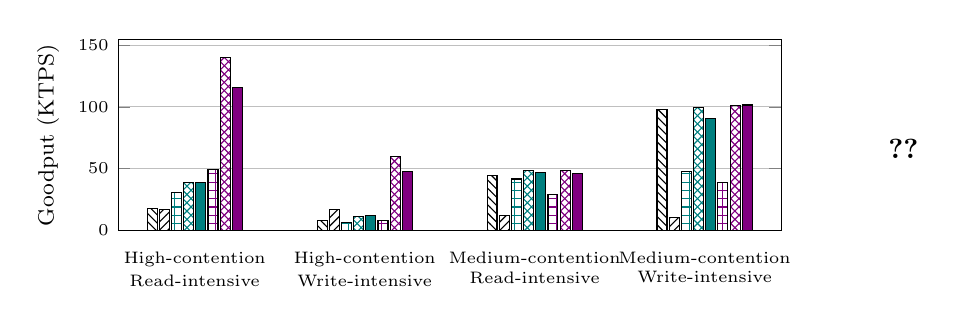
\begin{tikzpicture}
            \begin{groupplot}[group style={group size=1 by 1,
                            /pgf/bar width=3.6pt},
                    height = 4cm,
                    width = 10cm,
                    ybar= 2*\pgflinewidth,
                    xtick=data,
                    xticklabels={
                            \shortstack{High-contention \\ Read-intensive},
                            \shortstack{High-contention \\ Write-intensive},
                            \shortstack{Medium-contention \\ Read-intensive},
                            \shortstack{Medium-contention \\ Write-intensive}
                        },
                    ticklabel style={font=\tiny},
                    ymajorgrids=true,
                    enlarge x limits = 0.15,
                    legend columns=1,
                    legend entries={{\tiny 2PL}, {\tiny OCC}, {\tiny STO-Disk}, {\tiny STO-Memory}, {\tiny STO-\sketchname}, {\tiny TicToc-Disk}, {\tiny TicToc-Memory}, {\tiny TicToc-\sketchname}},
                    area legend,
                    legend to name=grouplegend,
                ]

                % graph [1,1] high
                \nextgroupplot[YCSBThroughputBarChartPlot, ylabel={Goodput (KTPS)}]
                \addplot[2PL-BarStyle] %2PL
                coordinates {(0,17.477367)
                        (1,7.801877)
                        (2,44.415733)
                        (3,98.0184)};
                \addplot[KR-OCC-BarStyle] %KR-OCC
                coordinates {(0,16.476967)
                        (1,16.502733)
                        (2,12.110933)
                        (3,9.95364)};
                \addplot[STO-Disk-BarStyle] %STO-Disk
                coordinates {(0,30.2847)
                        (1,6.549243)
                        (2,41.467833)
                        (3,47.448567)};
                \addplot[STO-Memory-BarStyle] %STO-Memory
                coordinates {(0,38.878867)
                        (1,11.258033)
                        (2,48.277933)
                        (3,99.339033)};
                \addplot[STO-FPSketch-BarStyle] %STO-FPSketch
                coordinates {(0,38.5077)
                        (1,11.6077)
                        (2,46.990067)
                        (3,90.8817)};
                \addplot[TicToc-Disk-BarStyle] %TicToc-Disk
                coordinates {(0,49.263467)
                        (1,8.097707)
                        (2,29.168467)
                        (3,38.399333)};
                \addplot[TicToc-Memory-BarStyle] %TicToc-Memory
                coordinates {(0,140.330333)
                        (1,59.562333)
                        (2,48.216233)
                        (3,100.82)};
                \addplot[TicToc-FPSketch-BarStyle] %TicToc-FPSketch
                coordinates {(0,115.33)
                        (1,47.927533)
                        (2,45.608067)
                        (3,101.462)};
                \coordinate (top) at (rel axis cs:0,1);% coordinate at top of the first plot
                \coordinate (bot) at (rel axis cs:1,0);% coordinate at bottom of the last plot
            \end{groupplot}
            \coordinate (c) at ($(top)!.5!(bot)$);

            \node[right=1cm, yshift=-5pt] at (c -| current bounding box.east) {\ref{grouplegend}};
        \end{tikzpicture}
    } \caption[Highlights of goodputs for YCSB workloads]{Performance
    comparison of various concurrency control mechanisms across different YCSB
    workloads, demonstrating the promise of in-memory timestamp ordering and the
    pitfalls of disk-based approaches. (Running 120 threads on NVMe SSD)}
    \label{fig:motivation}
\end{figure}

\Cref{fig:motivation} evaluates YCSB workloads, modified to execute transactions
in parallel, spanning contention (high, medium) and access patterns (read- vs.
write-intensive). It reports goodput, the throughput of successfully committed
transactions, to discount wasted work from aborts. The evaluation compares 2PL,
OCC, and two timestamp-based methods (STO and TicToc), each under three
timestamp placement strategies: stored on disk, in an idealized in-memory exact
timestamp store, and the proposed approximate timestamp store (\sketchname with
32KiB). This bracketing (Disk vs. Memory) with \sketchname\ in between isolates
the core tradeoff—CPU efficiency of timestamp-based methods versus the I/O and
lookup costs of materializing per-key timestamps on disk—while holding hardware
constant. The observed goodput gaps motivate approximate timestamping to achieve
near-in-memory performance with a minimal memory footprint.


\paragraph{The Promise (TicToc-Memory):} When timestamps are stored in an idealized
in-memory hash table, advanced protocols like TicToc dramatically outperform
traditional 2PL and OCC. TicToc-Memory achieves the highest throughput across
all workloads, with particularly impressive performance in high-contention
scenarios, demonstrating the immense potential of timestamp-based schemes.

\paragraph{The Pitfall (TicToc-Disk):} When these same timestamps are stored on
disk, the I/O overhead becomes so crippling that performance collapses, often
falling far below that of 2PL and OCC, especially in write-intensive workloads.
The performance gap between Memory and Disk variants is particularly pronounced
for write-intensive workloads, where the Query/Insert Asymmetry has the greatest
impact.

\paragraph{The Opportunity:} This stark contrast between the in-memory and
on-disk variants perfectly frames the research problem. It establishes a clear
need for a solution that can deliver the high performance of the in-memory
approach without its prohibitive memory cost. The results from STO-\sketchname
and TicToc-\sketchname, which use the proposed approximate timestamping
technique, demonstrate that such a solution is achievable, setting the stage for
the detailed presentation of this approach in the following chapters.


\chapter{\sketchname: Approximate Timestamp Storage for Timestamp-Based Concurrency Control}
\label{chapter:three}
This chapter introduces the concept of \emph{approximate timestamp storage} for
enabling efficient timestamp-based concurrency control (CC) mechanisms in modern
on-disk key-value stores. Exact timestamp storage systems are costly to maintain
at large scale, especially when data does not fit entirely in main memory. We
detail the key properties that an approximate timestamp storage system must
possess to preserve correctness—specifically serializability—for three common CC
protocols: STO~\cite{bernstein1987concurrency}, MVTO~\cite{reed1983mvto}, and
TicToc~\cite{yu2016tictoc}. We further describe the design and implementation of
\sketchname, a novel approximate timestamp storage approach. Through careful
analysis, we demonstrate that the overapproximation guarantees provided by
\sketchname are sufficient for correctness, while significantly improving
efficiency and scalability. Our approach unlocks new possibilities for
optimizing disk-based storage systems without sacrificing correctness guarantees
required by transactional workloads.



\section{Approximate Timestamp Storage}
\label{sec:requirements}

While timestamp-based CC mechanisms assume the guarantees of a \emph{map} for
storing their read and write timestamps, where a \emph{get} returns the latest
\emph{put}, here we show that for STO, MVTO, and TicToc such strong guarantees
are not necessary to ensure serializability. Specifically, we show that an
\emph{approximate timestamp storage} system with the following two properties
allows all three CC mechanisms to function correctly without any algorithmic
changes.

\begin{property}
    The approximate timestamp storage system can return an
    \emph{overapproximated} value for the timestamps it stores, only if there is
    no on-going transaction that has previously accessed the respective
    timestamps.
    \label{property_one}
\end{property}


\begin{property}
    When storing pairs of timestamps (read and write timestamps), if the CC
    mechanism stores only pairs for which their write timestamp is not larger
    than the read timestamp, then the approximate timestamp storage ensures
    that, for every pair of (overapproximated) timestamps it returns, the write
    timestamp is not larger than the read timestamp.
    \label{property_two}
\end{property}

STO assigns a serialization time $\tau$ to each transaction when the transaction
begins (see \Cref{alg:sto} for reference).  STO aborts a transaction if $\tau <
t_k$, where $t_k$ is the timestamp of a key $k$ that is being accessed.
Intuitively, since the comparison is always checking that $\tau$ is
\emph{smaller} than one of the key's timestamps, overapproximating key
timestamps can only cause transactions to abort. We make this more formal with a
simulation argument.  Suppose STO with approximate timestamp storage processes
transactions $T_1, \ldots, T_n$.  Consider STO with exact timestamp storage
processing the same set of transactions with the same ordering of their
operations.  Suppose that STO with exact timestamps has the additional property
that it aborts any transaction that STO with approximate timestamp storage
aborts.  This version of STO still guarantees serializability.  So, if we can
show that it would commit all the transactions that approximate STO would
commit, then this would mean that approximate STO is also serializable.  STO
only ever does \emph{put($k, \tau$)}, i.e. the only timestamps that it stores in
the timestamp storage engine are the timestamps assigned to transactions.  Thus
the sequence of \emph{put} operations performed by approximate and exact STO
will be identical. Hence every \emph{get} performed in approximate STO will
return a value at least as large as the one returned in exact STO
(\Cref{property_one}).  This implies that every timestamp check that causes an
abort in exact STO will also cause an abort in approximate STO.  Hence
approximate STO is serializable.

For MVTO's correctness, as long as timestamp overapproximation does not change
the original timestamp ordering of the versions for any record, the same
argumentation as for STO applies.

For TicToc, a simulation argument does not appear to be feasible, but the
original TicToc proof~\citep{yu2016tictoc} continues to work, even for
approximate timestamp storage.  This is because the proof reasons almost
entirely about timestamp inequalities across physical time, and approximate
timestamp storage will preserve those inequalities. We only need the following
lemma for approximate timestamp storage in order to make the original TicToc
proof go through:
\begin{lemma}
    Each timestamp increases monotonically in physical time in TicToc
    with approximate timestamp storage.  Furthermore, every write to a key $k$
    causes $k$'s write timestamp to increase.
\end{lemma}
\begin{proof}
    We establish the second fact first.  Consider a committing transaction that
    writes to $k$.  TicToc guarantees that, when the transaction performs
    \emph{put}$(k.wts, \tau)$ during its commit phase, $\tau$ is larger than the
    read timestamp returned by a previous \emph{get}$(k.rts)$ performed by the
    same transaction.  By \Cref{property_two}, $k.wts \leq k.rts$ at the time of
    the \emph{get} and, since the transaction references $k$ for the entire
    duration between the \emph{get} and \emph{put}, the approximate timestamp
    storage cannot spontaneously increase $k.wts$ during that interval.
    Furthermore, the transaction holds a lock on $k$ the entire time between the
    \emph{get} and the \emph{put}, so no other transaction could have performed
    a \emph{put} on $k.wts$.  Hence $k.wts$ cannot change between the
    transaction's \emph{get} and its \emph{put}, ensuring that the \emph{put}
    increases $k.wts$.

    The above argument also shows that, when a transaction performs
    \emph{put}$(k.rts,\tau)$ in its commit phase, it does not decrease $k.rts$.

    A transaction that reads $k$ may also update $k.rts$ during its validation
    phase, but this trivially does not decrease $k.rts$ because the transaction
    does \emph{put}$(k.rts, \max(\tau,$\emph{get}$(k.rts)))$ in an atomic
    section.

    Thus \emph{put} operations can never decrease a key's timestamps. The only
    other way a timestamp can change is through approximation, which is
    guaranteed not to decrease a timestamp (\Cref{property_one}). Thus
    timestamps increase monotonically over physical time.
\end{proof}

The two facts established in the above lemma are sufficient to enable TicToc's
original proof of serializability to go through.

In the next section, we design an approximate timestamp storage data structure
that meets the above requirements.




\section{\sketchname}
\label{sec:design}

\begin{wrapfigure}{r}{0.4\textwidth}
    \centering
    \includegraphics[width=.4\textwidth]{FPSketch.png}
    \caption[Overview of \sketchname]{\sketchname consists of the foveated region (hash table) storing accurate timestamps for active keys, peripheral region (sketch) for approximated timestamps, and the eviction mechanism transferring data between them.}
    \label{fig:FPSketch}
\end{wrapfigure}

In this section, we describe \sketchname, an approximate timestamp storage
structure that meets the requirements identified in \Cref{sec:requirements}.

As shown in \Cref{fig:FPSketch}, \sketchname consists of two regions: a
``foveated'' region providing accurate timestamps and a lossy ``peripheral''
region that maintains overapproximated timestamps. \Sketchname is a hybrid data
structure comprising both a hash table for the foveated region and a sketch for
the peripheral region. Additionally, the \sketchname uses an \emph{eviction
mechanism} to move timestamps from the foveated region to the peripheral one.

\paragraph{Hash table:} The hash table stores timestamps of keys that are
currently being accessed, ensuring that \sketchname does not spontaneously
increase the timestamps of these keys. Each record in the hash table has a
reference count, and each transaction increments the reference count the first
time it accesses a record and decrements it upon commit/abort. Only keys for
which the reference count reaches zero may be evicted from the hash table to the
sketch. Depending on the eviction mechanism chosen, these keys may either be
evicted immediately or kept in the hash table until evicted due to space
pressure using, e.g. LRU.

\begin{algorithm}[h!]
    \small
    \begin{algorithmic}
        \Struct{Sketch}
        \DeclareVar{int}{rows, cols}
        \DeclareVar{value}{table[rows][cols]}
        \Comment{\textbf{value} must support atomic ops.}
        \DeclareVar{uint64}{seeds[rows]}
        \EndStruct
    \end{algorithmic}

    \begin{algorithmic}[1]
        \Procedure{\timestampmax}{{\textsc{timestamps $t_1$}}, {\textsc{timestamps $t_2$}}}
        \Assign{$(\wts{v}, \rts{v})$}{$(MAX(\wts{t_1}, \wts{t_2}), MAX(\rts{t_1}, \rts{t_2}))$}
        \State \Return $v$
        \EndProcedure
        \Procedure{\timestampmin}{{\textsc{timestamps $t_1$}}, {\textsc{timestamps $t_2$}}}
        \Assign{$(\wts{v}, \rts{v})$}{$(MIN(\wts{t_1}, \wts{t_2}), MIN(\rts{t_1}, \rts{t_2}))$}
        \State \Return $v$
        \EndProcedure

        \Procedure{Put}{key $k$, value $v$}
        \For{$row = 0$ to $rows-1$}
        \Assign{$col$}{\hash{$k$}{$seeds[row]$} $\mod cols$}
        \Assign{$current\_value$}{\atomicload{$\&table[row][col]$}}
        \Assign{$is\_success$}{false}
        \While{!$is\_success$}
        \Assign{$new\_value$}{\timestampmaxfunc{$current\_value$}{$v$}} \label{alg:sketch-funcs:timestampmax}
        \Assign{$is\_success$}{\atomiccas{$\&table[row][col]$}{$\&current\_value$}{$new\_value$}}
        \EndWhile
        \EndFor
        \EndProcedure

        \Procedure{Get}{key $k$}
        \Assign{$col$}{\hash{$k$}{$seeds[0]$} $\mod cols$}
        \Assign{$value$}{\atomicload{$\&table[0][col]$}}
        \For{$row = 1$ to $rows-1$}
        \Assign{$col$}{\hash{$k$}{$seeds[row]$} $\mod cols$}
        \Assign{$current\_value$}{\atomicload{$\&table[row][col]$}}
        \Assign{$value$}{\timestampminfunc{$current\_value$}{$value$}} \label{alg:sketch-funcs:timestampmin}
        \EndFor
        \State \Return $value$
        \EndProcedure
    \end{algorithmic}
    \caption[Pseudocode of Sketch's \textsc{Put} and \textsc{Get}]{Pseudocode of Sketch's \textsc{Put} and \textsc{Get} functions using atomic operations.}
    \label{alg:sketch-funcs}
    \label{alg:timestamps-func}
\end{algorithm}

\paragraph{Sketch:} Timestamps evicted from the hash table are not discarded;
instead, they are stored in the sketch. \Cref{alg:sketch-funcs} provides
pseudocode for the \textsc{Put} and \textsc{Get} functions of the sketch,
utilizing atomic operations. The core logic is analogous to the count-min
sketch, except it takes $\max$ instead of incrementing during \textsc{Put}
operations, which guarantees \Cref{property_one}. For STO, MVTO, and TicToc,
timestamps are ordered pairs $(wts, rts)$ of write and read timestamps,
respectively.  The sketch takes field-wise $\max$ and $\min$, as shown in
\Cref{alg:timestamps-func}. Note that field-wise $\max$ and $\min$ preserve that
$wts\leq rts$, so our sketch preserves \Cref{property_two}.

When considering the memory limitations for both the hash table and the sketch
within the \sketchname framework, it's important to note that the hash table's
memory usage is directly tied to the quantity of keys currently accessed in
parallel. Conversely, the size of the sketch is predetermined and remains
constant based on the configured number of rows and columns, with the number of
rows aligning with the number of hash functions employed.

\subsection{\sketchname Operations}


\begin{algorithm}[h!]
    \small
    \begin{algorithmic}
        \Struct{\sketchname{}}
        \DeclareVar{HashTable}{hashtable}
        \DeclareVar{Sketch}{sketch}
        \EndStruct
    \end{algorithmic}

    \begin{algorithmic}[1]
        \Procedure{IncRef}{key $k$}
        \Assign{$e$}{\hashtableget{$k$}}
        \If{$e = NULL$}
        \Assign{$ts$}{\sketchget{$k$}}
        \State \hashtableput{$k$}{$ts$}
        \Comment Initialize $refcount = 1$
        \State \Call{Evict}{\null}
        \Else
        \State{$e.refcount++$}
        \EndIf
        \EndProcedure


        \Procedure{DecRef}{key $k$}
        \Assign{$e$}{\hashtableget{$k$}}
        \Comment{$e$ cannot be NULL}
        \State{$e.refcount--$}
        \If{$e.refcount = 0$}
        \State \Call{Evict}{\null}
        \EndIf
        \EndProcedure

        \Procedure{Get}{key $k$}
        \State \Return \hashtableget{$k$}.ts
        \EndProcedure

        \Procedure{Put}{key $k$, timestamp $ts$}
        \Assign{\hashtableget{$k$}$.ts$}{$ts$}
        \EndProcedure

        \Procedure{Evict}{\null}
        \Assign{$E$}{\{$item$ in \textit{hashtable} | $item.val.refcount = 0$\}}
        \Comment Only choose to evict from the set of keys that are not in-use
        \ForAll{$item$ in \textsc{toEvictPolicy}($E$)}
        \State \sketchput{$item.k$}{$item.val.ts$}
        \State \hashtableremove{$item.k$}
        \EndFor
        \EndProcedure


    \end{algorithmic}
    \caption[Pseudocode of \sketchname operations]{Pseudocode of \sketchname operations. The pseudocode assumes linearizability using locks.}
    \label{alg:operations}
\end{algorithm}

\sketchname provides four operations, as shown in \Cref{alg:operations}:
\textsc{Get}, \text{Put}, \textsc{IncRef}, and \textsc{DecRef}. \textsc{IncRef}
and \textsc{DecRef} increment and decrement the refcounts on keys in the
\sketchname, and may need to transfer timestamps between the hashtable and the
sketch. Transactions are required to call $\textsc{IncRef}(k)$ before their
first access to a key $k$, through a \textsc{Get} or \textsc{Put} operation, and
should not access the key after calling $\textsc{DecRef}(k)$. Although we omit
locking from the pseudocode, all operations ensure linearizability for each item
in the hash table through the use of per-bucket locks.

\textbf{\textsc{IncRef}}  allocates a hashtable slot for $k$ if one does not
already exist, initializes its timestamp from the sketch, and sets its refcount
to 1.  Otherwise it just increments the refcount of the existing entry.
\textsc{IncRef} executes atomically via a lock on the hashtable bucket.

\textbf{\textsc{DecRef}} looks up the key in the hashtable, which is
guaranteed to exist due to the prior \textsc{IncRef}, and it decrements the
entry's refcount. Again, this sequence of operations is executed atomically by
using per-bucket locks on the hashtable. If the refcount reached 0, it calls the
eviction method that implements the chosen eviction mechanism. The eviction
mechanism may only evict keys for which refcount is 0, and it implements an
eviction policy, \textsc{toEvictPolicy}, which selects which of these keys to
evict.

\textbf{\textsc{Get} and \textsc{Put}} just return or update the timestamps
in the hashtable entry, which is guaranteed to exist due to the prior call to
\textsc{IncRef}.



\subsection{\sketchname Variants}
\label{sec:design:variants}

\sketchname allows customizable sizes for both its regions; this customization
exposes the trade-off between timestamp accuracy and space. Increasing the size
of either of these regions also increases the overall accuracy of the
timestamps, but the space consumption for the accuracy boost varies across the
two regions. In this chapter we explore two \sketchname variants: \Fsketchname,
which favors a large foveated region, and \Psketchname which, in contrast,
favors a large peripheral region. More precisely, given a fixed size space, $S$,
that can be used to store the timestamps of the keys that are not in-use,
\Fsketchname allocates most of $S$ for the foveated region, while \Psketchname
allocates most of $S$ for the peripheral region, as we detail further. For
\Psketchname, we provide intution on how to size the sketch (in terms of the
number of rows and columns) in the next section.

\textbf{\Fsketchname} is a variant of \sketchname that uses the smallest
possible sketch, a sketch of size one, and allocates all the remaining available
space to the hashtable. This variant uses the CLOCK eviction mechanism to evict
timestamps from the hashtable when it runs out of space to store timestamps of
keys that are not in-use.

\textbf{\Psketchname} is a variant of \sketchname that uses the smallest
possible hashtable by implementing an aggressive eviction policy that evicts a
key from the hashtable as soon as its refcount reaches 0 (i.e., is no longer
in-use by any on-going transaction). All the available space is allocated to the
sketch.

\subsection{Sizing \sketchname}

In this section, we give a simple heuristic argument that the size of the sketch
should be proportional to $\Theta(CK)$ columns and $\Theta(\log CK)$ rows, where
$C$ is the average number of concurrent transactions and $K$ is the average
number of keys accessed by each transaction. Thus the total size of the sketch
need be at most $O(CK \log CK)$.

We argue that, if the sketch is large enough, then, during the entirety of some
transaction $T$'s execution, the sketch will not spontaneously increase the
timestamps of any of the keys accessed by $T$.  Let $A_T$ be the set of keys
accessed by \textit{any} transaction during $T$'s execution. Note that the
average size of $A_T$ is around $CK$.  If the sketch has $CK$ columns then,
within each row, a constant fraction of the keys will not collide with any other
key in $A_T$.  Since there are $\Theta(\log CK)$ rows, with high probability
every key is collision-free in at least one row. Thus the sketch will not make
any new approximation errors on any of the keys in $A_T$ during $T$'s execution.

So, most of the time, the system will behave as if it is using exact timestamp
storage during a transaction $T$'s execution.  We just have to argue that
approximation errors made before $T$ begins won't affect whether $T$ aborts.
This is straightforward from examining each CC mechanism.  For example, STO
compares timestamps of keys only with $T$'s timestamp, $\tau$.  All keys have
timestamps less than $\tau$ before $T$ begins, so the only way $T$ can abort is
if some other transaction updates a timestamp of a key accessed by $T$.  But
then $T$ would have aborted in a system with exact timestamps, as well. Similar
arguments can be made for TicToc and MVTO.

Note this analysis is merely a heuristic rule of thumb.  It assumes that the
transactions do not try to cause aborts. A malicious actor could attempt to
discover colliding keys (by issuing transactions on different keys and seeing
which ones abort) and then issue a sequence of transactions that it knows will
all abort due to hash collisions in the sketch.  Second, it ignores the fact
that, if a transaction aborts due to a timestamp approximation, that may allow
another transaction to commit, which in turn may cause another transaction to
abort, and so on.  So it is not strictly true that timestamp approximations
cannot affect future transactions.  However, this effect is not likely to be
significant.  Finally, it ignores variance in the sizes and concurrency of
transactions, which may necessitate larger sketches, and it ignores skew in
key-access patterns, which may allow much smaller sketches.


As for the hashtable, recall that the hashtable needs to hold only active keys,
and so it should be sized to hold roughly $\Theta(CK)$ keys, as well.  In
practice, we would advise using a resizable hashtable and simply letting it grow
as needed. Several state-of-the-art hashtables support concurrent operations
while resizing~\cite{iceberg, dash, dlht}, so this need not cause any hiccups in
throughput.

\subsection{\sketchname Implementation}

We implement the hash table of \sketchname on top of IcebergHT~\cite{iceberg}
and the sketch from scratch. We modified IcebergHT to perform reference-count
management and to support holding bucket locks across multiple operations. For
the \Fsketchname variant that uses a sketch of size one, we use an optimized
version \Cref{alg:sketch-funcs} which no longer needs to compute hashes.


\section{Integration with the Existing CC Algorithms}
\label{sec:integration}

In this section, we describe how to integrate \sketchname into STO, MVTO, and
TicToc. STO and MVTO differ substantially from TicToc in that TicToc verifies
transactions post-execution in an optimistic manner, whereas STO and MVTO can
abort transactions mid-execution. All three maintain read and write timestamps
per key (per version in MVTO's case).

\subsection{TicToc}

\begin{algorithm}[htbp]
    \small
    \begin{algorithmic}[1]
        \Procedure{Read}{database $D$, \sketchname $S$, transaction $T$, key $k$}
        \Atomic
        \If{$k\not\in T.R$}
        \State $S$.\textsc{IncRef}($k$)
        \EndIf
        \Assign{$T.R[k]$}{$S$.\textsc{Get}($k$)}
        \Assign{$T.R[k].data$}{$D$.\textsc{Read}($k$)}
        \Comment{Read $k$'s value from disk}
        \EndAtomic
        \State \Return $T.R[k].data$
        \EndProcedure
        \Procedure{Validate}{transaction $T$}
        \For{$k \in T.W$ in sorted order}
        \State \lock $k$
        \State $S$.\textsc{IncRef}($k$)
        \EndFor
        \Assign{$T$.\commitTime}{0}
        \Comment{Compute our commit timestamp $T$.\commitTime}
        \For{$k \in  T.W \cup T.R$}
        \If{$k \in T.W$}
        \Assign{$T$.\commitTime}{$\max(T.\commitTime, 1 + S.\textsc{Get}(k).rts)$}
        \Else
        \Assign{$T$.\commitTime}{$\max(T.\commitTime, T.R[k].wts)$}
        \EndIf
        \EndFor
        \For{$k \in T.R$}
        \Atomic
        \If{$T.R[k].rts < T.\commitTime$}
        \If{$T.R[k].wts \not= S.\textsc{Get}(k).wts \vee (S.\textsc{Get}(k).rts \leq T.\commitTime \wedge \locked(k) \wedge k \not\in T.W)$} \label{alg:tictoc:abort-test}
        \State \abort \label{alg:tictoc:abort}
        \Else
        \Assign{$curr$}{$S.\textsc{Get}(k)$}
        \Assign{$curr.rts$}{$\max(T.\commitTime, curr.rts)$}
        \State $S.\textsc{Put}(k, curr)$
        \EndIf
        \EndIf
        \EndAtomic
        \EndFor
        \EndProcedure
        \Procedure{Commit}{database $D$, \sketchname $S$, transaction $T$}
        \For{$k \in T.W$}
        \State $D.\textsc{Write}(k, T.W[k].data)$
        \Comment{Write $k$'s value to disk}
        \State $S.\textsc{Put}(k, (T.\commitTime, T.\commitTime))$
        \State $S.\textsc{DecRef}(k)$ \label{alg:tictoc:remove}
        \State \unlock $k$ \label{alg:tictoc:unlock}
        \EndFor
        \For{$k\in T.R$}
        \State $S.\textsc{DecRef}(k)$
        \EndFor
        \EndProcedure
    \end{algorithmic}
    \caption[TicToc integrated with \sketchname]{TicToc integrated with \sketchname. Each transaction $T$
        maintains a read set $R$ and a write set $W$. TicToc buffers write
        values in the write set $W$ until commit time.}
    \label{alg:tictoc}
\end{algorithm}

\Cref{alg:tictoc} shows the pseudocode for TicToc with \sketchname. There are
only two changes to the algorithm. First, timestamps are stored in the
\sketchname instead of inline with the tuples, as in the original TicToc paper,
so the syntax for accessing timestamps is different.  Second, we need to call
\textsc{IncRef} and \textsc{DecRef} when a transaction first accesses a key and
when it finishes.  Note that all the logic for dealing with timestamp
approximation is encapsulated within the \sketchname code---TicToc is not aware
of the approximations.

Transactions increment a key's refcount the first time they access it, and
decrement it only during commit (or as part of the abort procedure, which is not
shown).  This ensures that the key's timestamps will not change spontaneously
due to approximations in the timestamp storage structure during the
transaction's execution. It then records the timestamps in the transaction's
read set, which is structured as a map from keys to timestamps.

The write set is a map from keys to data items.  When a transaction writes to a
key, we just record the specified key-value pair in the transaction's write set.
Note that a transaction doesn't need to check the timestamps of a key in its
write set until validation time, as in the original TicToc. Although not shown
explicitly, the full implementation checks the transaction's write set during
reads so that a transaction sees its own writes.

TicToc requires a mechanism to lock keys during transaction validation.
Although this is abstracted in our pseudocode, in our implementation this is
accomplished by having a lock bit in a key's entry in the timestamp hash table.

When a transaction either commits or aborts, it is essential to unlock the write
set and decrease the reference counts of the accessed keys. It's worth noting
that we omit the code for finalizing transactions upon abort due to space
constraints. However, the steps involved in unlocking and removing entries for
transaction aborts are the same as those outlined in \Cref{alg:tictoc:unlock}
and \Cref{alg:tictoc:remove}.

\subsection{STO}

\begin{algorithm}[htbp]
    \small
    \begin{algorithmic}[1]
        \Procedure{Begin}{global timestamp $*c$, transaction $T$}
        \Assign{$T$.\commitTime}{\atomicfetchadd{$c$}{1}} \EndProcedure

        \Procedure{Read}{database $D$, \sketchname $S$, transaction $T$, key $k$}
        \If{$k\not\in T.R$}
        \State \textsc{ReadLock} $k$
        \Assign{$T.R$}{$T.R\cup\{k\}$}
        \State $S$.\textsc{IncRef}($k$)
        \If{$T.\commitTime < S.\textsc{Get}(k).wts$} \label{alg:sto:abort1-check}
        \State \abort \label{alg:sto:abort1}
        \EndIf
        \Atomic
        \Assign{$curr$}{$S.\textsc{Get}(k)$}
        \Assign{$curr.rts$}{$\max(T.\commitTime, curr.rts)$}
        \State $S.\textsc{Put}(k, curr)$
        \EndAtomic
        \Assign{$T.R[k].data$}{$D$.\textsc{Read}($k$)}
        \Comment{Read $k$'s value from disk}
        \State \unlock $k$
        \EndIf
        \State \Return $T.R[k].data$

        \EndProcedure
        \Procedure{Write}{database $D$, \sketchname $S$, transaction $T$, key $k$, val $v$}
        \If{$k\not\in T.W$}
        \State \textsc{WriteLock} $k$
        \State $S$.\textsc{IncRef}($k$)
        \If{($T.\commitTime < S.\textsc{Get}(k).wts) \vee (T.\commitTime < S.\textsc{Get}(k).rts)$}
        \State \abort \label{alg:sto:abort3}
        \EndIf
        \Assign{$curr$}{$S.\textsc{Get}(k)$}
        \Assign{$curr.wts$}{$\max(T.\commitTime, curr.wts)$}
        \State $S.\textsc{Put}(k, curr)$
        \EndIf
        \Assign{$T.W[k]$}{$v$}
        \EndProcedure
        \Procedure{Commit}{database $D$, \sketchname $S$, transaction $T$}
        \For{$k \in T.R$}
        \State $S.\textsc{DecRef}(k)$
        \EndFor
        \For{$k \in T.W$}
        \State $D$.\textsc{Write}($k$, $T.W[k]$)
        \Comment{Write $k$'s value to disk}
        \State $S.\textsc{DecRef}(k)$
        \State \unlock $k$
        \EndFor
        \EndProcedure
    \end{algorithmic}
    \caption[STO integrated with \sketchname]{STO integrated with \sketchname. Each transaction $T$
        maintains a read set $R$ and a write set $W$.}
    \label{alg:sto}
\end{algorithm}

\Cref{alg:sto} shows the pseudocode of STO with \sketchname. The
changes are similar to those in TicToc.

STO assigns each transaction a commit timestamp when it begins. Whenever a
transaction reads or writes an entry in the database, STO locks that key, checks
that the key's timestamps are compatible with the commit timestamp of the
transaction, and then updates the key's timestamps. STO does not allow
transactions to access uncommitted data. This can be achieved with read-write
locks, as illustrated in \Cref{alg:sto}. We implemented these locks with ``dirty
bits''\cite{wolf2015sto}. With dirty bits, readers do not block writers,
enabling more concurrency than in 2PL. Dirty bits work as follows. When a writer
updates a tuple, it sets the tuple's dirty bit to 1. This blocks subsequent
readers and writers until the writing transaction commits or aborts.  Readers,
however, use the dirty bit only as a latch to atomically read the tuple into a
private buffer, and hence do not block subsequent writers (or, obviously,
subsequent readers).

As in our TicToc implementation, we store the reader-writer locks in the entries
in the \sketchname. Although not shown explicitly, if a transaction writes a key
after reading it, it needs to be able to atomically upgrade its reader lock to a
a writer lock.  If upgrading is not possible, the transaction aborts.

Note that STO needs to update the timestamps in the sketch only the first time a
transaction accesses a key, since the timestamp updates performed by a
transaction using STO are idempotent.  During a read, we need to read and write
the timestamps in the sketch atomically, since other readers may also be
updating the key's read timestamp. This isn't necessary for writes, since the
transaction already holds an exclusive lock on the key.

To commit, a transaction needs only to write its data back to the database,
release all references to entries in the timestamp storage structure, and unlock
all the keys.  Aborting, not shown, is similar.

\subsection{MVTO}
\label{sec:fpsketch:mvto}

In a standard MVTO system, the database may maintain multiple versions of each
key-value pair---a new version is created whenever a transaction commits a write
to the respective key.  Each version has associated timestamps and, when a
transaction first reads a key, it looks through the versions to find one whose
timestamps make it visible to that transaction and uses that version.  If the
transaction cannot find a compatible version (e.g. if the old versions have
already been garbage collected) then it must abort.

As we noted in \Cref{sec:requirements}, MVTO requires that the approximate
timestamp storage system must maintain the relative timestamp ordering of the
versions of a key-value-pair.  We satisfy this requirement by ensuring that our
system approximates the timestamps of only the most recent version of any
key-value pair.

Specifically, our MVTO implementation works as follows.  When a key is inactive,
we store the (approximate) timestamps of the most recent version of that key in
\sketchname.  When the key becomes active, we copy the timestamps of the most
recent version from \sketchname into the hashtable.  Whenever a new version of
the key is created, we store the timestamps of the new version in the hashtable,
as well.  Once the key becomes inactive, we move the timestamps of the most
recent version back to \sketchname and discard the timestamps of all the older
versions.

Whenever a new version is created, it is assigned a monotonically increasing
version number and stored in SplinterDB indexed as (key, version-number)
$\rightarrow$ value.  Each entry in the hashtable also contains the version
number so, once a transaction finds an entry with compatible timestamps in the
hashtable, it learns the version number that it needs in order to look up that
version of the key-value pair in SplinterDB using a point lookup.

When a transaction accesses an inactive key, however, the sketch can tell the
transaction only the timestamps of the most recent version, but not its version
number.  Thus the transaction does not know what version number to use to look
up the key in SplinterDB.  We considered two solutions to this problem.  The
first was to have the transaction perform a predecessor query in SplinterDB,
i.e. to query for the predecessor of (key, $\infty$).  However, predecessor
queries in SplinterDB are slower than point queries because predecessor queries
cannot use SplinterDB's maplets~\cite{ConwayFaJo23}.

To avoid predecessor queries, we implemented the following optimization.
Whenever a new version of a key-value pair is inserted into SplinterDB, we also
insert the same key-value pair into SplinterDB with the special version number
0, i.e. we maintain the invariant that the most recent version of a key is
always stored as (key, 0).  This incurs two insertions into SplinterDB for each
version, but enables queries of inactive keys to perform point queries instead
of range queries.  Overall, we found this approach offered higher performance,
so this is the scheme we use in all our benchmarks.


\paragraph{Persistence and crash safety:} It is possible to handle crashes using
standard techniques like write-ahead logging and checkpoints. Note that we do
not need to persist the timestamps across crashes or shutdowns since there can
be no serializability violations between transactions that execute before and
after a crash or shutdown.



\section{Evaluation}\label{sec:eval}

We evaluate the effectiveness of \sketchname in scaling timestamp-based CC
mechanisms to on-disk databases. There are five high-level take-aways from our
experiments:
\setlist{nolistsep}
\begin{itemize}
    \item \sketchname-based versions of STO, MVTO, and TicToc outperform
          versions that keep timestamps on disk in all our experiments, often by
          dramatic margins.  For example, \sketchname improves TicToc goodput by
          up to 5.9x, STO by up to 1.8x, and MVTO by over 160x.
    \item Similarly, \psketchname-based protocols can offer up to 2x greater
          goodput than \fsketchname-based ones. Furthermore, TicToc and STO with
          \psketchname are never substantially slower than the \fsketchname
          variants.
    \item The goodputs of TicToc and STO with \sketchname are close to an
          idealized algorithm, which assumes we can fit all timestamp metadata
          in RAM, across diverse workloads.
    \item TicToc-\psketchname in particular outperforms 2PL and OCC across the
          board.
    \item \sketchname requires a tiny amount of memory -- 32KiB in our
          experiments with an 80GB database.
\end{itemize}
In summary, \sketchname offers essentially strictly improved performance with
little to no downside for STO, MVTO, and TicToc across a wide range of
benchmarks.


\subsection{Experimental Setup}
\label{sec:eval-setup}

We run our experiments on a CloudLab~\cite{duplyakin2019cloudlab} Clemson r6525
machine with two 32-core AMD 7543 at 2.8GHz, 256GB memory, and one 1.6TB PCIe
v4.0 NVMe SSD.

We use SplinterDB, a fast, scalable write-optimized key-value store, as the
underlying storage system for the concurrency control mechanisms we consider in
this evaluation. We configure SplinterDB to use the raw device I/O (with the
DIRECT\_IO flag) to avoid the filesystem overhead. We size SplinterDB's internal
cache to a percentage of each workload's database size, as we detail below.

In all our experiments, we utilize 120 threads, which is the maximum supported
by the version of SplinterDB used in this work. Each thread executes
transactions in a closed loop. When a transaction aborts, it can be retried up
to 5 times. The retry mechanism uses exponential backoff. We tuned the initial
backoff interval for each scheme by initially setting it to be roughly twice the
average uncontended transaction completion time, and then tuned it until the
abort rate roughly matched that of the Memory variant.

We measure Goodput in Kilo Transactions Per Second (KTPS) and also evaluate the
abort rate. Goodput represents the number of successfully committed transactions
per second. The abort rate is calculated as the ratio of the total number of
aborts, which can be up to 6 per transaction (including the initial attempt and
5 retries), to the total number of attempted transactions, which is the sum of
all aborts and commits.


\subsubsection{Concurrency-Control Mechanisms}

We implement and evaluate several CC mechanisms, including all three
timestamp-based CCs described in~\Cref{sec:background:timestamp-based-cc} (STO,
MVTO, and TicToc), and two classic CCs which are widely used in disk-based
databases: two-phase locking (2PL) and Kung-Robinson Optimistic Concurrency
Control (OCC). Unlike timestamp-based CCs, these two classic mechanisms do not
require maintaining per-record metadata, thus avoiding disk I/O overhead for
metadata access. For 2PL, we employ a no-wait policy after evaluating multiple
deadlock prevention mechanisms (including wound-wait and wound-die). We selected
no-wait due to its generally good performance in our experiments, which aligns
with findings from previous
works~\cite{DBLP:conf/sigmod/RenFA16,DBLP:conf/usenix/TangE18}.

We implement five variants of STO, MVTO, and TicToc. These variants are
distinguished by their methods for storing and accessing per-record timestamps,
which range from relying entirely on disk to using fully in-memory solutions.

First, we establish the performance boundaries with two baseline variants:
\begin{itemize}
    \item \emph{Disk}: This is the simplest approach. Timestamps are stored on
          disk as part of each record, requiring an I/O operation for every
          timestamp access.

    \item \emph{Memory}: This represents a theoretical upper bound on
          performance. It stores timestamps for all keys in a single, large
          in-memory hash table. While fast, this approach is generally
          impractical due to its prohibitive memory requirements.
\end{itemize}

The remaining three variants maintain an in-memory hash table to store the keys
of currently active transactions. They differ primarily in how they manage
timestamps for the much larger set of inactive keys:
\begin{itemize}
    \item \emph{Disk-Cache}: This variant enhances the Disk approach by adding a
          cache for inactive keys, inspired by PostgreSQL's SLRU
          cache~\cite{postgresql-slru}, buffering on-disk metadata. It uses the
          same active-key hash table as the sketch variants. For inactive keys,
          it employs a 32 KiB in-memory cache with a CLOCK eviction policy to
          buffer timestamps read from disk. This cache operates alongside
          SplinterDB's standard page caching. We also explore the impact of
          larger caches in \Cref{sec:ycsb}.

    \item \emph{\fsketchname}: As one variant of \sketchname, described in
          \Cref{sec:design:variants}, it supplements the active-key hash table
          with an additional 32 KiB of memory dedicated to storing timestamps
          for inactive keys. Also, a CLOCK eviction policy is employed.

    \item \emph{\psketchname}: The other variant of \sketchname also uses the
          active-key hash table but employs a 32 KiB probabilistic sketch for
          managing inactive key timestamps. The sketch is configured with 2 rows
          to balance space efficiency and error rates~\cite{flexswitch}, with
          the number of columns set to fit the memory budget.
\end{itemize}

\begin{figure}[!t]
    \centering
    \resizebox{\textwidth}{!}{%
        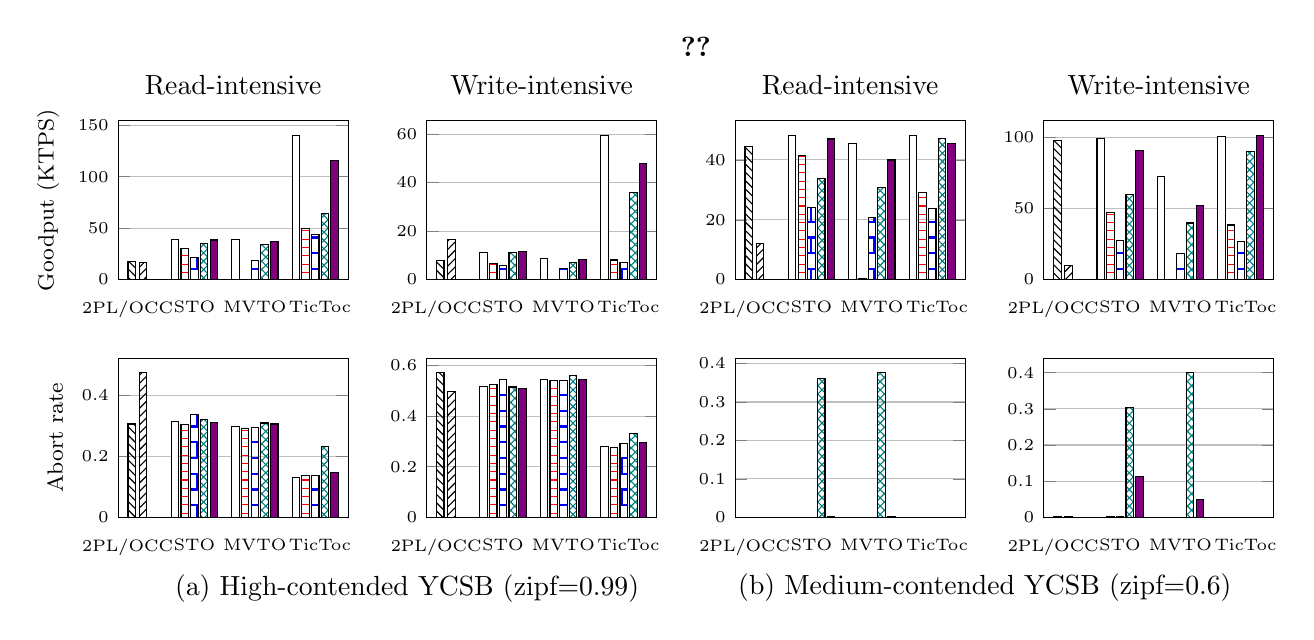
\begin{tikzpicture}
            \begin{groupplot}[group style={group size=4 by 2,
                            /pgf/bar width=2.7pt},
                    height = 3.6cm,
                    width = 4.5cm,
                    ybar= 2*\pgflinewidth,
                    xtick={-1, 0.425, 1.7125, 3.1},
                    xticklabels={2PL/OCC, STO, MVTO, TicToc},
                    ymajorgrids=true,
                    enlarge x limits = 0.2,
                    legend columns=-1,
                    legend entries={{\ssmall Memory (Idealized)}, {\ssmall Disk}, {\ssmall Disk-Cache}, {\ssmall \fsketchname},  {\ssmall \psketchname}},
                    area legend,
                    legend to name=grouplegend,
                ]

                % graph [1,1] high
                \nextgroupplot[title={Read-intensive},YCSBThroughputBarChartPlot, ylabel={Goodput (KTPS)}]
                \addplot[2PL-BarStyle, forget plot] coordinates {(-0.5, 17.477367)};
                \addplot[KR-OCC-BarStyle, forget plot] coordinates {(-0.26, 16.476967)};
                \addplot[Memory-BarStyle] coordinates {(0.425, 38.878867) (1.7125, 38.669267) (3, 140.330333)};
                \addplot[Disk-BarStyle] coordinates {(0.425, 30.2847) (1.7125, 0.507507) (3, 49.263467)};
                \addplot[Disk-Cache-BarStyle] coordinates {(0.425, 21.507167) (1.7125, 19.000767) (3, 43.443867)};
                \addplot[Counter-Lazy-BarStyle] coordinates {(0.425, 34.837367) (1.7125, 33.990467) (3, 63.942467)};
                \addplot[FPSketch-BarStyle] coordinates {(0.425, 38.5077) (1.7125, 36.797133) (3, 115.33)};
                \coordinate (top) at (rel axis cs:0,1);% coordinate at top of the first plot

                % graph [1,3] high
                \nextgroupplot[title={Write-intensive}, YCSBThroughputBarChartPlot]
                \addplot[2PL-BarStyle, forget plot] coordinates {(-0.5, 7.801877)};
                \addplot[KR-OCC-BarStyle, forget plot] coordinates {(-0.26, 16.502733)};
                \addplot[Memory-BarStyle] coordinates {(0.425, 11.258033) (1.7125, 8.60338) (3, 59.562333)};
                \addplot[Disk-BarStyle] coordinates {(0.425, 6.549243) (1.7125, 0.224855) (3, 8.097707)};
                \addplot[Disk-Cache-BarStyle] coordinates {(0.425, 5.843353) (1.7125, 4.63059) (3, 7.08267)};
                \addplot[Counter-Lazy-BarStyle] coordinates {(0.425, 11.186667) (1.7125, 7.12615) (3, 35.785433)};
                \addplot[FPSketch-BarStyle] coordinates {(0.425, 11.6077) (1.7125, 8.470803) (3, 47.927533)};

                % graph [1,1] medium
                \nextgroupplot[title={Read-intensive},YCSBThroughputBarChartPlot]
                \addplot[2PL-BarStyle, forget plot] coordinates {(-0.5, 44.415733)};
                \addplot[KR-OCC-BarStyle, forget plot] coordinates {(-0.26, 12.110933)};
                \addplot[Memory-BarStyle] coordinates {(0.425, 48.277933) (1.7125, 45.4553) (3, 48.216233)};
                \addplot[Disk-BarStyle] coordinates {(0.425, 41.467833) (1.7125, 0.345895) (3, 29.168467)};
                \addplot[Disk-Cache-BarStyle] coordinates {(0.425, 24.1369) (1.7125, 20.6195) (3, 23.9132)};
                \addplot[Counter-Lazy-BarStyle] coordinates {(0.425, 33.744567) (1.7125, 30.869233) (3, 47.0563)};
                \addplot[FPSketch-BarStyle] coordinates {(0.425, 46.990067) (1.7125, 39.9891) (3, 45.608067)};


                % graph [1,3] medium
                \nextgroupplot[title={Write-intensive},YCSBThroughputBarChartPlot]
                \addplot[2PL-BarStyle, forget plot] coordinates {(-0.5, 98.0184)};
                \addplot[KR-OCC-BarStyle, forget plot] coordinates {(-0.26, 9.95364)};
                \addplot[Memory-BarStyle] coordinates {(0.425, 99.339033) (1.7125, 72.628067) (3, 100.82)};
                \addplot[Disk-BarStyle] coordinates {(0.425, 47.448567) (1.7125, 0.329319) (3, 38.399333)};
                \addplot[Disk-Cache-BarStyle] coordinates {(0.425, 27.401467) (1.7125, 18.576433) (3, 27.043833)};
                \addplot[Counter-Lazy-BarStyle] coordinates {(0.425, 59.674867) (1.7125, 39.79) (3, 89.918167)};
                \addplot[FPSketch-BarStyle] coordinates {(0.425, 90.8817) (1.7125, 51.949233) (3, 101.462)};
                \coordinate (bot) at (rel axis cs:1,0);% coordinate at bottom of the last plot

                % graph [1,2] read intensive
                \nextgroupplot[AbortRateBarChartPlot, ylabel={Abort rate}]
                \addplot[2PL-BarStyle, forget plot] coordinates {(-0.5, 0.305736)};
                \addplot[KR-OCC-BarStyle, forget plot] coordinates {(-0.26, 0.473590)};
                \addplot[Memory-BarStyle] coordinates {(0.425, 0.313093) (1.7125, 0.296428) (3, 0.129434)};
                \addplot[Disk-BarStyle] coordinates {(0.425, 0.304782) (1.7125, 0.291449) (3, 0.136846)};
                \addplot[Disk-Cache-BarStyle] coordinates {(0.425, 0.337739) (1.7125, 0.292974) (3, 0.136776)};
                \addplot[Counter-Lazy-BarStyle] coordinates {(0.425, 0.319974) (1.7125, 0.309124) (3, 0.233345)};
                \addplot[FPSketch-BarStyle] coordinates {(0.425, 0.311677) (1.7125, 0.305936) (3, 0.146853)};

                % graph [1,4] write intensive
                \nextgroupplot[AbortRateBarChartPlot]
                \addplot[2PL-BarStyle, forget plot] coordinates {(-0.5, 0.571029)};
                \addplot[KR-OCC-BarStyle, forget plot] coordinates {(-0.26, 0.498173)};
                \addplot[Memory-BarStyle] coordinates {(0.425, 0.516916) (1.7125, 0.544745) (3, 0.281149)};
                \addplot[Disk-BarStyle] coordinates {(0.425, 0.525495) (1.7125, 0.539769) (3, 0.274822)};
                \addplot[Disk-Cache-BarStyle] coordinates {(0.425, 0.544414) (1.7125, 0.539943) (3, 0.292887)};
                \addplot[Counter-Lazy-BarStyle] coordinates {(0.425, 0.514934) (1.7125, 0.559506) (3, 0.331628)};
                \addplot[FPSketch-BarStyle] coordinates {(0.425, 0.507419) (1.7125, 0.546395) (3, 0.295353)};

                % graph [1,2]
                \nextgroupplot[AbortRateBarChartPlot]
                \addplot[2PL-BarStyle, forget plot] coordinates {(-0.5, 0.000319)};
                \addplot[KR-OCC-BarStyle, forget plot] coordinates {(-0.26, 0.000167)};
                \addplot[Memory-BarStyle] coordinates {(0.425, 0.000093) (1.7125, 0.000092) (3, 0.000029)};
                \addplot[Disk-BarStyle] coordinates {(0.425, 0.000085) (1.7125, 0.000062) (3, 0.000036)};
                \addplot[Disk-Cache-BarStyle] coordinates {(0.425, 0.000087) (1.7125, 0.000093) (3, 0.00003)};
                \addplot[Counter-Lazy-BarStyle] coordinates {(0.425, 0.361786) (1.7125, 0.375866) (3, 0.000106)};
                \addplot[FPSketch-BarStyle] coordinates {(0.425, 0.002301) (1.7125, 0.000815) (3, 0.000087)};

                % graph [1,4]
                \nextgroupplot[AbortRateBarChartPlot]
                \addplot[2PL-BarStyle, forget plot] coordinates {(-0.5, 0.002547)};
                \addplot[KR-OCC-BarStyle, forget plot] coordinates {(-0.26, 0.001037)};
                \addplot[Memory-BarStyle] coordinates {(0.425, 0.000513) (1.7125, 0.000435) (3, 0.000213)};
                \addplot[Disk-BarStyle] coordinates {(0.425, 0.00141) (1.7125, 0.000536) (3, 0.00031)};
                \addplot[Disk-Cache-BarStyle] coordinates {(0.425, 0.001389) (1.7125, 0.000541) (3, 0.000348)};
                \addplot[Counter-Lazy-BarStyle] coordinates {(0.425, 0.303408) (1.7125, 0.399625) (3, 0.00059)};
                \addplot[FPSketch-BarStyle] coordinates {(0.425, 0.113349) (1.7125, 0.048471) (3, 0.00048)};

            \end{groupplot}
            \coordinate (c) at ($(top)!.5!(bot)$);
            \coordinate (cc1) at ($(top)!.25!(bot)$);
            \coordinate (cc2) at ($(top)!.75!(bot)$);

            \node[above] at (c |- current bounding box.north) {\ref{grouplegend}};
            \node[below] at (cc1 |- current bounding box.south) {(a) High-contended YCSB (zipf=0.99)};
            \node[above] at (cc2 |- current bounding box.south) {(b) Medium-contended YCSB (zipf=0.6)};
        \end{tikzpicture}
    }
    \caption[YCSB small-transaction workloads results]{YCSB small-transaction workloads results with 120 processing threads. In write-intensive workloads, each transaction performs 8 reads and 8 writes. In read-intensive workloads, each transaction performs 15 reads and 1 write. Note that, in the medium-contended workload, several schemes have abort rates very close to 0.}
    \label{fig:ycsb}
\end{figure}


\subsubsection{Workloads} 

We use two benchmarks to evaluate the performance of the
CCs we implement: (1) YCSB~\cite{ycsb}, which models large-scale online
services, and (2) TPC-C~\cite{tpcc}, the industry standard for evaluating OLTP
systems.


In the YCSB workloads, we first load a dataset of 673 million key-value pairs,
with 24-byte keys and 100-byte values. This loading phase is performed before
every run, followed by the execution phase. To evaluate \sketchname's across
diverse scenarios, we execute seven YCSB workloads: four ``small'' transaction
workloads, two ``mixed'' transaction workloads, and one ``large'' transaction
workload.  Each of the small workloads is either \emph{read-intensive} or
\emph{write-intensive}. In write-intensive workloads, transactions perform 8
reads and 8 writes. In read-intensive workloads, transactions perform 15 reads
and 1 write. The keys used in these transactions are generated based on a
Zipfian distribution. Each of the workloads is either \emph{high-contention} or
\emph{medium-contention}.  For the high-contention workloads the Zipfian
distribution uses \emph{theta}=0.99 (10\% of the pairs are accessed by ~80\% of
the operations). For the medium-contention workloads, \emph{theta}=0.6 (10\% of
the pairs are accessed by ~40\% of all the operations). The ``mixed''
transaction workloads consist of a mix of small transactions (reading and
writing 2 keys each) and medium-sized transactions, which read 28 keys each. For
these workloads, the Zipfian \emph{theta} values of 0.9 and 0.6 are used for
high- and medium-contention, respectively. Finally, we run a high-contention
(Zipfian 0.9) ``large'' transaction workload, where 5\% of the transactions read
1000 keys, and the remaining transactions each read and write 8 keys.
SplinterDB's internal cache is 6GiB, which is less than 10\% of the database
size. We run YCSB experiments over a duration of 240 seconds. We repeat each run
three times and report average numbers.

As in many previous works, we evaluated TPC-C workloads that comprise only two
of the five transaction types in TPC-C, namely \texttt{Payment} and
\texttt{NewOrder}, with each type making up 50\% of the workload.  These two
transaction types constitute 88\% of the default TPC-C mix and are the most
interesting for our evaluation. We ran the TPC-C workloads for various number of
warehouses, 4, 8, 16, and 32, which dictate the initial database size and the
contention level. SplinterDB's internal cache was configured to 256MB. The TPC-C
experiments are run for 120 seconds and repeated three times to minimize noise
caused by random variation.

\subsection{YCSB Results}
\label{sec:ycsb}


\subsubsection{Small-Transaction Workloads}

\Cref{fig:ycsb} shows the goodput and abort rates for all our timestamp-based CC
mechanisms on our four small-transaction YCSB workloads.

One important result from \Cref{fig:ycsb} is that in all scenarios, integrating
\sketchname with the timestamp-based CCs enables them to substantially
outperform their ``Disk'' and ``Disk-Cache'' counterparts. Except with MVTO,
which we discuss below, Disk-Cache is slightly slower than Disk due to the
overhead of managing the extra cache. We provide a deeper dive on how cache size
affects Disk-Cache's performance in another experiment described below. The STO
and MVTO variants match their ``Memory'' counterparts. TicToc experiences
performance penalties from aborts because validation occurs after optimistically
executing all operations, requiring them to be re-executed. This effect is
particularly pronounced for read operations. Nevertheless, TicToc with
\sketchname still achieve the best performance across our workloads. The
\psketchname-based protocols also match or outperform their \fsketchname-based
variants on these workloads.

We can draw several other conclusions from these results.

\setlist{nolistsep}
\begin{itemize}
    \item TicToc variants generally outperform not only 2PL/OCC but also their
          STO and MVTO analogues, due to TicToc's advanced timestamp-based
          scheme.
    \item Disk-based variants are substantially slower, due to I/O to fetch
          timestamps. I/O overhead is particularly pronounced in write-intensive
          workloads because, as explained in \Cref{sec:background:motivation},
          reads bring in the timestamps ``for free'' but writes to SplinterDB do
          not cause the old value (and hence the old timestamps) to be read into
          cache. Consequently, Disk-based variants incur reads for every write,
          incurring high overhead in write-intensive workloads.
    \item The gap between Disk-based and other variants is also larger in the
          medium-contended workloads because these workloads have less locality,
          increasing cache miss rates.
    \item MVTO-Disk is also particularly slow because it stores old versions on
          disk and uses a range query to find the most recent version whenever
          it needs to bring a key into cache. Range queries are slower than
          point queries because range queries do not use filters to avoid I/O in
          SplinterDB. In contrast, MVTO-Disk-Cache is able to utilize the same
          \textit{V0} technique as our \sketchname-basedMVTO variants, which
          enables it to use point queries instead of range queries to bring keys
          into cache.  As a result, MVTO-Disk-Cache substantially outperforms
          MVTO-Disk.
\end{itemize}


\begin{figure}[!t]
    \centering
    \resizebox{\textwidth}{!}{%
        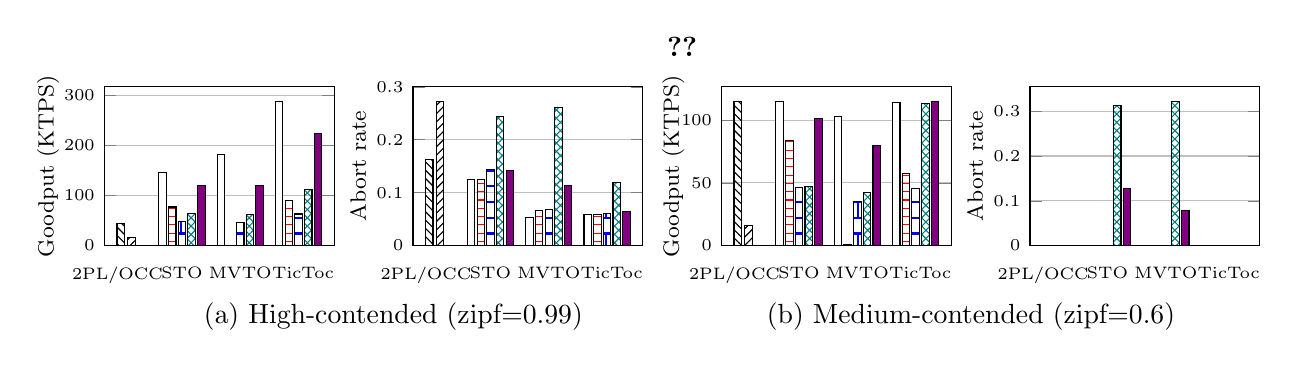
\begin{tikzpicture}
            \begin{groupplot}[group style={group size=4 by 1,
                            /pgf/bar width=2.7pt},
                    height = 3.6cm,
                    width = 4.5cm,
                    ybar= 2*\pgflinewidth,
                    xtick={-1, 0.425, 1.7125, 3.1},
                    xticklabels={2PL/OCC, STO, MVTO, TicToc},
                    ymajorgrids=true,
                    enlarge x limits = 0.225,
                    legend columns=-1,
                    legend entries={{\ssmall Memory (Idealized)}, {\ssmall Disk}, {\ssmall Disk-Cache}, {\ssmall \fsketchname},  {\ssmall \psketchname}},
                    area legend,
                    legend to name=grouplegend,
                ]

                % graph [1,1] high
                \nextgroupplot[YCSBThroughputBarChartPlot, ylabel={Goodput (KTPS)}, ylabel style={yshift=-5pt}]
                \addplot[2PL-BarStyle, forget plot] coordinates {(-0.5, 44.788867)};
                \addplot[KR-OCC-BarStyle, forget plot] coordinates {(-0.26, 16.090133)};
                \addplot[Memory-BarStyle] coordinates {(0.425, 145.850667) (1.7125, 181.95) (3, 288.844333)};
                \addplot[Disk-BarStyle] coordinates {(0.425, 77.255) (1.7125, 0.669773) (3, 90.075633)};
                \addplot[Disk-Cache-BarStyle] coordinates {(0.425, 48.505933) (1.7125, 46.451467) (3, 63.239933)};
                \addplot[Counter-Lazy-BarStyle] coordinates {(0.425, 63.550667) (1.7125, 62.2656) (3, 112.575333)};
                \addplot[FPSketch-BarStyle] coordinates {(0.425, 119.693333) (1.7125, 120.718) (3, 224.293)};
                \coordinate (top) at (rel axis cs:0,1);% coordinate at top of the first plot

                % graph [2,1] abort rate
                \nextgroupplot[AbortRateBarChartPlot, ylabel={Abort rate}, ylabel style={yshift=-3pt}]
                \addplot[2PL-BarStyle, forget plot] coordinates {(-0.5, 0.162746)};
                \addplot[KR-OCC-BarStyle, forget plot] coordinates {(-0.26, 0.272886)};
                \addplot[Memory-BarStyle] coordinates {(0.425, 0.124274) (1.7125, 0.052306) (3, 0.058323)};
                \addplot[Disk-BarStyle] coordinates {(0.425, 0.125071) (1.7125, 0.066406) (3, 0.058108)};
                \addplot[Disk-Cache-BarStyle] coordinates {(0.425, 0.143426) (1.7125, 0.06801) (3, 0.060623)};
                \addplot[Counter-Lazy-BarStyle] coordinates {(0.425, 0.243168) (1.7125, 0.261633) (3, 0.118915)};
                \addplot[FPSketch-BarStyle] coordinates {(0.425, 0.141617) (1.7125, 0.113494) (3, 0.064861)};

                % graph [3,1] medium
                \nextgroupplot[YCSBThroughputBarChartPlot, ylabel={Goodput (KTPS)}, ylabel style={yshift=-8pt}]
                \addplot[2PL-BarStyle, forget plot] coordinates {(-0.5, 114.436)};
                \addplot[KR-OCC-BarStyle, forget plot] coordinates {(-0.26, 15.946)};
                \addplot[Memory-BarStyle] coordinates {(0.425, 114.518) (1.7125, 102.656667) (3, 114.271667)};
                \addplot[Disk-BarStyle] coordinates {(0.425, 83.553) (1.7125, 0.640778) (3, 57.3336)};
                \addplot[Disk-Cache-BarStyle] coordinates {(0.425, 46.006033) (1.7125, 35.193433) (3, 45.397667)};
                \addplot[Counter-Lazy-BarStyle] coordinates {(0.425, 47.0387) (1.7125, 42.445667) (3, 113.193333)};
                \addplot[FPSketch-BarStyle] coordinates {(0.425, 101.459) (1.7125, 79.5607) (3, 115.063)};

                % graph [4,1] medium abort rate
                \nextgroupplot[AbortRateBarChartPlot, ylabel={Abort rate}, ylabel style={yshift=-3pt}]
                \addplot[2PL-BarStyle, forget plot] coordinates {(-0.5, 0.000793)};
                \addplot[KR-OCC-BarStyle, forget plot] coordinates {(-0.26, 0.000174)};
                \addplot[Memory-BarStyle] coordinates {(0.425, 0.000557) (1.7125, 0.000091) (3, 0.000358)};
                \addplot[Disk-BarStyle] coordinates {(0.425, 0.000203) (1.7125, 0.000052) (3, 0.000076)};
                \addplot[Disk-Cache-BarStyle] coordinates {(0.425, 0.000182) (1.7125, 0.000183) (3, 0.000067)};
                \addplot[Counter-Lazy-BarStyle] coordinates {(0.425, 0.312689) (1.7125, 0.322235) (3, 0.000367)};
                \addplot[FPSketch-BarStyle] coordinates {(0.425, 0.128001) (1.7125, 0.078421) (3, 0.000441)};
                \coordinate (bot) at (rel axis cs:1,0);% coordinate at bottom of the last plot

            \end{groupplot}
            \coordinate (c) at ($(top)!.5!(bot)$);
            \coordinate (cc1) at ($(top)!.25!(bot)$);
            \coordinate (cc2) at ($(top)!.75!(bot)$);

            \node[above] at (c |- current bounding box.north) {\ref{grouplegend}};
            \node[below] at (cc1 |- current bounding box.south) {(a) High-contended (zipf=0.99)};
            \node[above] at (cc2 |- current bounding box.south) {(b) Medium-contended (zipf=0.6)};
        \end{tikzpicture}
    }
    \caption[YCSB mixed-transaction workloads results]{YCSB mixed-transaction workloads results with 120 processing threads. 80\% of transactions perform 2 reads and 2 writes, and 20\% of transactions perform 28 reads. Note that, in the medium-contended workload, several schemes have abort rates very close to 0.}
    \label{fig:ycsb:mixed}
\end{figure}


\subsubsection{Mixed-Transaction Workloads} 

\Cref{fig:ycsb:mixed} shows the goodput and abort rates for our timestamp-based
CC mechanisms on our mixed-transaction workloads. Several of the same
observations apply here, as well: TicToc variants generally perform better than
all other variants, 2PL, and OCC; Disk variants are substantially slower; and
MVTO-Disk suffers in particular due to its use of range queries when bringing a
key into cache. In high-contention workloads, STO and MVTO implementations with
\psketchname demonstrate higher goodput compared to 2PL and OCC. However, in
medium-contention scenarios, they experience performance degradation due to
unnecessary aborts caused by timestamp approximation. Additionally,
MVTO-\psketchname incurs extra overhead from maintaining a special V0 version.
These workloads also show that the \psketchname-based variants consistently
substantially outperform their \fsketchname-based variants. TicToc-\psketchname,
STO-\psketchname, and MVTO-\psketchname have about 50\% greater goodput than
their \fsketchname variants, respectively. This advantage stems from
\psketchname's ability to maintain more accurate timestamp approximations
compared to \fsketchname, resulting in fewer unnecessary aborts.


\begin{figure}[!t]
    \centering
    \resizebox{.75\textwidth}{!}{%
        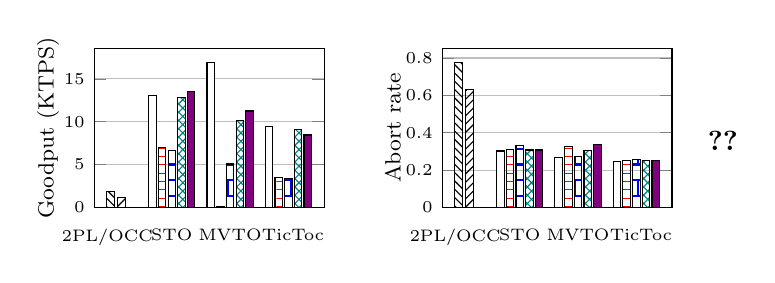
\begin{tikzpicture}
            \begin{groupplot}[group style={
                            group size=2 by 1,
                            horizontal sep=1.5cm,
                            /pgf/bar width=2.7pt
                        },
                    height = 3.6cm,
                    width = 4.5cm,
                    ybar= 2*\pgflinewidth,
                    xtick={-1, 0.425, 1.7125, 3.1},
                    xticklabels={2PL/OCC, STO, MVTO, TicToc},
                    ymajorgrids=true,
                    enlarge x limits = 0.225,
                    legend columns=1,
                    legend entries={{\ssmall Memory (Idealized)}, {\ssmall Disk}, {\ssmall Disk-Cache}, {\ssmall \fsketchname},  {\ssmall \psketchname}},
                    area legend,
                    legend to name=grouplegend,
                ]

                % graph [1,1] high
                \nextgroupplot[YCSBThroughputBarChartPlot, ylabel={Goodput (KTPS)}, ylabel style={yshift=-5pt}]
                \addplot[2PL-BarStyle, forget plot] coordinates {(-0.5, 1.83184)};
                \addplot[KR-OCC-BarStyle, forget plot] coordinates {(-0.26, 1.154507)};
                \addplot[Memory-BarStyle] coordinates {(0.425, 13.078167) (1.7125, 16.861367) (3, 9.470163)};
                \addplot[Disk-BarStyle] coordinates {(0.425, 7.000837) (1.7125, 0.067857) (3, 3.49488)};
                \addplot[Disk-Cache-BarStyle] coordinates {(0.425, 6.60874) (1.7125, 5.065917) (3, 3.351893)};
                \addplot[Counter-Lazy-BarStyle] coordinates {(0.425, 12.855333) (1.7125, 10.172537) (3, 9.09105)};
                \addplot[FPSketch-BarStyle] coordinates {(0.425, 13.5421) (1.7125, 11.255833) (3, 8.450747)};
                \coordinate (top) at (rel axis cs:0,1);% coordinate at top of the first plot

                % graph [1,2] abort rate
                \nextgroupplot[AbortRateBarChartPlot, ylabel={Abort rate}, ylabel style={yshift=-5pt}]
                \addplot[2PL-BarStyle, forget plot] coordinates {(-0.5, 0.773841)};
                \addplot[KR-OCC-BarStyle, forget plot] coordinates {(-0.26, 0.633733)};
                \addplot[Memory-BarStyle] coordinates {(0.425, 0.302199) (1.7125, 0.268966) (3, 0.247955)};
                \addplot[Disk-BarStyle] coordinates {(0.425, 0.310228) (1.7125, 0.325941) (3, 0.249079)};
                \addplot[Disk-Cache-BarStyle] coordinates {(0.425, 0.333103) (1.7125, 0.270333) (3, 0.254321)};
                \addplot[Counter-Lazy-BarStyle] coordinates {(0.425, 0.307612) (1.7125, 0.304549) (3, 0.249676)};
                \addplot[FPSketch-BarStyle] coordinates {(0.425, 0.307297) (1.7125, 0.33709) (3, 0.252645)};
                \coordinate (bot) at (rel axis cs:1,0);% coordinate at bottom of the last plot

            \end{groupplot}
            \coordinate (c) at ($(top)!.5!(bot)$);

            \node[right=4cm] at (c |- current bounding box.east) {\ref{grouplegend}};
        \end{tikzpicture}
    } \caption[YCSB long-transaction workloads results]{YCSB long-transaction
    workloads results with 120 processing threads. 5\% of transactions perform
    1000 reads and the rest of transactions perform 8 writes and 8 reads. The
    distribution is Zipfian with 0.9.}
    \label{fig:ycsb:long}
\end{figure}

\subsubsection{Long-Transaction Workload}

\Cref{fig:ycsb:long} shows our final YCSB workload, which includes some long
transactions that read 1000 keys.  Most of the trends here are similar to the
other YCSB  workloads.

The main take-away is that STO and TicToc with approximate timestamp storage
work just as well as their Memory variants, demonstrating that approximate
timestamps can handle large transactions, not just small ones.

\begin{figure}[!t]
    \centering
    \resizebox{.75\textwidth}{!}{%
        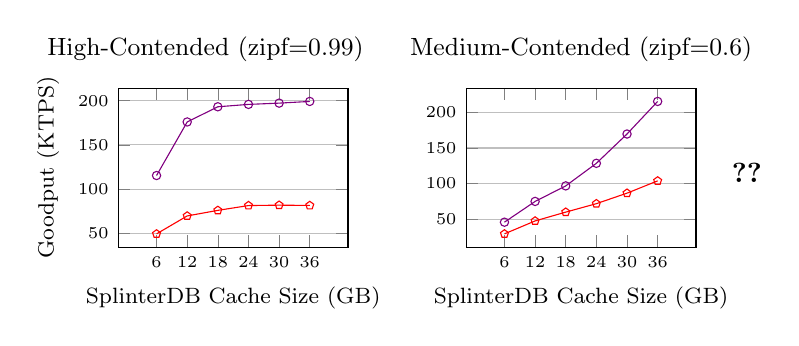
\begin{tikzpicture}
            \begin{groupplot}[group style={
                            group size=2 by 1,
                            horizontal sep=1.5cm
                        },
                    height = 3.6cm,
                    width = 4.5cm,
                    xtick=data,
                    ymajorgrids=true,
                    enlarge x limits = 0.25,
                    legend columns=1,
                    legend entries={{\ssmall \psketchname}, {\ssmall Disk}},
                    legend to name=grouplegend,
                    label style={font=\footnotesize},
                    ticklabel style={font=\ssmall},
                ]

                % graph [1,1] high
                \nextgroupplot[title={\small{High-Contended (zipf=0.99)}}, title style={xshift=-10pt}, xlabel={SplinterDB Cache Size (GB)}, ylabel={Goodput (KTPS)}]
                \addplot[FPSketch-LineStyle] coordinates {(6, 115.33) (12, 175.96) (18, 193.158333) (24, 195.850333) (30, 197.279667) (36, 199.209)};
                \addplot[Disk-LineStyle] coordinates {(6, 49.263467) (12, 69.5672) (18, 75.883167) (24, 81.314367) (30, 81.7691) (36, 81.4466)};
                \coordinate (top) at (rel axis cs:0,1);% coordinate at top of the first plot

                % graph [1,1] medium
                \nextgroupplot[title={\small{Medium-Contended (zipf=0.6)}}, xlabel={SplinterDB Cache Size (GB)}]
                \addplot[FPSketch-LineStyle] coordinates {(6, 45.608067) (12, 74.820133) (18, 96.687467) (24, 128.449) (30, 169.679) (36, 215.528)};
                \addplot[Disk-LineStyle] coordinates {(6, 29.168467) (12, 47.3736) (18, 59.791367) (24, 71.666667) (30, 86.460567) (36, 103.74)};
                \coordinate (bot) at (rel axis cs:1,0);% coordinate at bottom of the last plot
            \end{groupplot}
            \coordinate (c) at ($(top)!.5!(bot)$);

            \node[right=4cm] at (c |- current bounding box.east) {\ref{grouplegend}};
        \end{tikzpicture}
    }
    \caption[TicToc Disk and \psketchname with varying SplinterDB Cache Size]{YCSB read-intensive small-transaction workloads for TicToc Disk and \psketchname with varying SplinterDB Cache Size.}
    \label{fig:ycsb:spl_cache}
\end{figure}



\subsubsection{Approximate Timestamp Storage Versus Caching}

\Cref{fig:ycsb:spl_cache} shows how varying the SplinterDB cache size affects
goodput of TicToc-Disk and TicToc-\psketchname.  The purpose of this experiment
is to answer the question: can we fix the performance problems in Disk-based
schemes by simply increasing cache sizes?

\Cref{fig:ycsb:spl_cache} suggest that the answer is ``No.''  In the
high-contended workload, TicToc-Disk with a 37 GiB cache is still slower than
TicToc-\psketchname with a mere 6GiB cache.  And in the medium-contended
workload, TicToc-Disk needs roughly twice as much cache to match the goodput of
TicToc-\psketchname, which needs only 32KiBs to store timestamps.

There are likely several reasons that database cache is not as effective as
in-memory approximate timestamp storage.  First, caches store disk blocks, which
may store numerous key-value-timestamp records.  So, in order to store a single
timestamp for a single key, the block cache will need to hold an entire disk
block, whereas approximate timestamp storage will need only a few bytes.  Thus
approximate timestamp storage just uses memory more efficiently. Second,
timestamp storage is optimized for quick, in-memory access, whereas database
caches can have high overheads due to locking, latching, and data structure
traversals, among other things.

\subsubsection{Metadata Memory Usage}

We now compare the memory used to store metadata in each scheme. The Memory
variant stored in RAM 40 bytes for each KV-pair: a 24-byte key and a 16-byte
structure containing a read timestamp, write timestamp, and a latch.  There were
673M keys in the database, so the Memory variant stored 27GiB of metadata.  The
Disk variant also stored 16 bytes of metadata with each 124-byte record in the
database.  All metadata was stored in SplinterDB's 6GiB cache, so the total
memory used for metadata was approximately 16 / (124 + 16) $\times$ 6 GiB
$\approx$ 685 MiB.  The Disk-Cache just adds a small 32KiB cache to the Disk
scheme and hence has similar memory usage. The \sketchname variants use a 32KiB
cache plus a hashtable of 40-byte entries for each active key, for a total
average memory usage of 160KiB.

\begin{figure}[!t]
    \centering
    \resizebox{.75\textwidth}{!}{%
        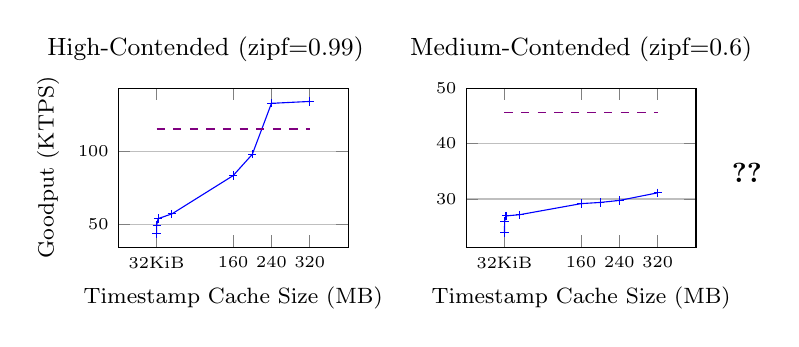
\begin{tikzpicture}
            \begin{groupplot}[group style={
                            group size=2 by 1,
                            horizontal sep=1.5cm
                        },
                    height = 3.6cm,
                    width = 4.5cm,
                    xtick=data,
                    log basis x=10,
                    ymajorgrids=true,
                    enlarge x limits = 0.25,
                    legend columns=-1,
                    legend entries={{\ssmall Disk-Cache}, {\ssmall \psketchname}},
                    legend to name=grouplegend,
                    label style={font=\footnotesize},
                    ticklabel style={font=\ssmall},
                    xtick={0.032, 160, 240, 320},
                    xticklabels={32KiB, 160, 240, 320},
                ]

                % graph [1,1] high
                \nextgroupplot[title={{\small High-Contended (zipf=0.99)}}, title style={xshift=-10pt}, xlabel={Timestamp Cache Size (MB)}, ylabel={Goodput (KTPS)}]
                \addplot[Disk-Cache-LineStyle] coordinates {(0.032, 43.443867) (0.32, 49.2635) (3.2, 53.8861) (32, 57.0798)
                        (160, 83.2997) (200, 97.8576) (240, 132.731) (320, 134.029)};
                \draw [dashed, color=violet, line width=0.6pt] (axis cs:0.032,115.33) -- (axis cs:320,115.33);
                \coordinate (top) at (rel axis cs:0,1);% coordinate at top of the first plot

                % graph [1,1] medium
                \nextgroupplot[title={{\small Medium-Contended (zipf=0.6)}}, xlabel={Timestamp Cache Size (MB)}, ymax=50]
                \addplot[Disk-Cache-LineStyle] coordinates {(0.032, 23.9132) (0.32, 25.9769) (3.2, 26.9321) (32, 27.1612)
                        (160, 29.1538) (200, 29.3707) (240, 29.7308) (320, 31.1101)};
                \draw [dashed, color=violet, line width=0.6pt] (axis cs:0.032,45.608067) -- (axis cs:320,45.608067);
                \coordinate (bot) at (rel axis cs:1,0);% coordinate at bottom of the last plot
            \end{groupplot}
            \coordinate (c) at ($(top)!.5!(bot)$);

            \node[right=4cm] at (c |- current bounding box.east) {\ref{grouplegend}};
        \end{tikzpicture}
    }
    \caption[TicToc Disk-Cache and \psketchname with 32KiB of sketch size]{YCSB read-intensive small-transaction workloads for TicToc Disk-Cache compared to \psketchname with 32KiB of sketch size (Dashed line).}
    \label{fig:ycsb:disk_cache}
\end{figure}


\subsubsection{Disk-Cache Versus \psketchname}

\Cref{fig:ycsb:disk_cache} compares the performance of Disk-Cache with
\psketchname. We used the same configuration for \psketchname--32KiB cache. The
dashed line is the goodput of \psketchname. In high-contended workloads,
Disk-Cache requires about 220MB of cache to achieve the same goodput as
\psketchname, which uses only 32KiB of memory. Disk-Cache never achieves the
same goodput as \psketchname in our medium-contended workloads because the
Disk-Cache variant still requires I/O to access timestamps, while \psketchname
does not.


\begin{figure*}[!t]
    \centering
    \resizebox{\textwidth}{!}{%
        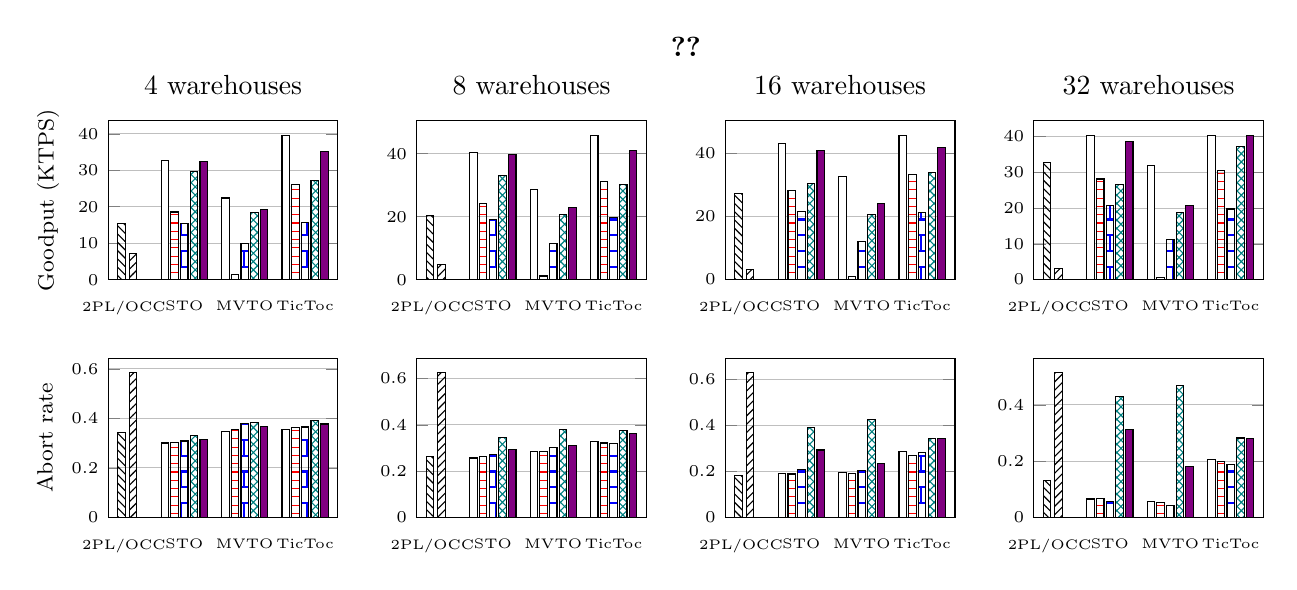
\begin{tikzpicture}
            \begin{groupplot}[group style={group size=4 by 2,
                            /pgf/bar width=2.7pt},
                    height = 3.6cm,
                    width = 4.5cm,
                    ybar= 2*\pgflinewidth,
                    xtick={-0.8625, 0.425, 1.7125, 3},
                    xticklabels={2PL/OCC, STO, MVTO, TicToc},
                    xticklabel style={font=\tiny},
                    ymajorgrids=true,
                    enlarge x limits = 0.2,
                    legend columns=-1,
                    legend entries={{\ssmall Memory (Idealized)}, {\ssmall Disk}, {\ssmall Disk-Cache}, {\ssmall \fsketchname},  {\ssmall \psketchname}},
                    area legend,
                    legend to name=grouplegend,
                ]

                % graph [1,1]
                \nextgroupplot[title={4 warehouses},YCSBThroughputBarChartPlot, ylabel={Goodput (KTPS)}]
                \addplot[2PL-BarStyle, forget plot] coordinates {(-0.5, 15.5001)};
                \addplot[KR-OCC-BarStyle, forget plot] coordinates {(-0.26, 7.206467)};
                \addplot[Memory-BarStyle] coordinates {(0.425, 32.585533) (1.7125, 22.4149) (3, 39.639567)};
                \addplot[Disk-BarStyle] coordinates {(0.425, 18.557367) (1.7125, 1.411917) (3, 26.220533)};
                \addplot[Disk-Cache-BarStyle] coordinates {(0.425, 15.341867) (1.7125, 9.981953) (3, 15.5759)};
                \addplot[Counter-Lazy-BarStyle] coordinates {(0.425, 29.750667) (1.7125, 18.412333) (3, 27.169833)};
                \addplot[FPSketch-BarStyle] coordinates {(0.425, 32.529233) (1.7125, 19.205733) (3, 35.212833)};
                \coordinate (top) at (rel axis cs:0,1);% coordinate at top of the first plot

                % graph [1,2]
                \nextgroupplot[title={8 warehouses}, YCSBThroughputBarChartPlot]
                \addplot[2PL-BarStyle, forget plot] coordinates {(-0.5, 20.284167)};
                \addplot[KR-OCC-BarStyle, forget plot] coordinates {(-0.26, 4.85534)};
                \addplot[Memory-BarStyle] coordinates {(0.425, 40.531467) (1.7125, 28.662767) (3, 45.897233)};
                \addplot[Disk-BarStyle] coordinates {(0.425, 24.197667) (1.7125, 1.168913) (3, 31.277167)};
                \addplot[Disk-Cache-BarStyle] coordinates {(0.425, 19.0729) (1.7125, 11.346067) (3, 19.727467)};
                \addplot[Counter-Lazy-BarStyle] coordinates {(0.425, 33.2235) (1.7125, 20.8041) (3, 30.266267)};
                \addplot[FPSketch-BarStyle] coordinates {(0.425, 39.8032) (1.7125, 22.932033) (3, 41.0892)};

                % graph [1,3]
                \nextgroupplot[title={16 warehouses},YCSBThroughputBarChartPlot]
                \addplot[2PL-BarStyle, forget plot] coordinates {(-0.5, 27.2005)};
                \addplot[KR-OCC-BarStyle, forget plot] coordinates {(-0.26, 3.224307)};
                \addplot[Memory-BarStyle] coordinates {(0.425, 43.0441) (1.7125, 32.64) (3, 45.766333)};
                \addplot[Disk-BarStyle] coordinates {(0.425, 28.275833) (1.7125, 0.965151) (3, 33.350267)};
                \addplot[Disk-Cache-BarStyle] coordinates {(0.425, 21.6463) (1.7125, 12.093367) (3, 21.253)};
                \addplot[Counter-Lazy-BarStyle] coordinates {(0.425, 30.3558) (1.7125, 20.678133) (3, 33.882967)};
                \addplot[FPSketch-BarStyle] coordinates {(0.425, 40.8327) (1.7125, 24.077067) (3, 41.9933)};


                % graph [1,4] 32wh
                \nextgroupplot[title={32 warehouses},YCSBThroughputBarChartPlot]
                \addplot[2PL-BarStyle, forget plot] coordinates {(-0.5, 32.723)};
                \addplot[KR-OCC-BarStyle, forget plot] coordinates {(-0.26, 3.22205)};
                \addplot[Memory-BarStyle] coordinates {(0.425, 40.381433) (1.7125, 31.824867) (3, 40.255467)};
                \addplot[Disk-BarStyle] coordinates {(0.425, 28.132067) (1.7125, 0.665631) (3, 30.495833)};
                \addplot[Disk-Cache-BarStyle] coordinates {(0.425, 20.6061) (1.7125, 11.3145) (3, 19.752167)};
                \addplot[Counter-Lazy-BarStyle] coordinates {(0.425, 26.470933) (1.7125, 18.868) (3, 37.3103)};
                \addplot[FPSketch-BarStyle] coordinates {(0.425, 38.500733) (1.7125, 20.832467) (3, 40.297567)};

                \coordinate (bot) at (rel axis cs:1,0);% coordinate at bottom of the last plot

                % graph [2,1] 4 wh
                \nextgroupplot[AbortRateBarChartPlot, ylabel={Abort rate}]
                \addplot[2PL-BarStyle, forget plot] coordinates {(-0.5, 0.341061)};
                \addplot[KR-OCC-BarStyle, forget plot] coordinates {(-0.26, 0.583609)};
                \addplot[Memory-BarStyle] coordinates {(0.425, 0.300203) (1.7125, 0.347864) (3, 0.355087)};
                \addplot[Disk-BarStyle] coordinates {(0.425, 0.303987) (1.7125, 0.356123) (3, 0.361833)};
                \addplot[Disk-Cache-BarStyle] coordinates {(0.425, 0.308412) (1.7125, 0.380381) (3, 0.364769)};
                \addplot[Counter-Lazy-BarStyle] coordinates {(0.425, 0.33226) (1.7125, 0.38239) (3, 0.392239)};
                \addplot[FPSketch-BarStyle] coordinates {(0.425, 0.313404) (1.7125, 0.366488) (3, 0.377045)};

                % graph [2,2] 8 wh
                \nextgroupplot[AbortRateBarChartPlot]
                \addplot[2PL-BarStyle, forget plot] coordinates {(-0.5, 0.261302)};
                \addplot[KR-OCC-BarStyle, forget plot] coordinates {(-0.26, 0.625084)};
                \addplot[Memory-BarStyle] coordinates {(0.425, 0.256733) (1.7125, 0.286516) (3, 0.329841)};
                \addplot[Disk-BarStyle] coordinates {(0.425, 0.262611) (1.7125, 0.28539) (3, 0.321566)};
                \addplot[Disk-Cache-BarStyle] coordinates {(0.425, 0.27151) (1.7125, 0.300326) (3, 0.320764)};
                \addplot[Counter-Lazy-BarStyle] coordinates {(0.425, 0.346327) (1.7125, 0.379734) (3, 0.374494)};
                \addplot[FPSketch-BarStyle] coordinates {(0.425, 0.293032) (1.7125, 0.312573) (3, 0.36223)};

                % graph [2,3] 16 wh
                \nextgroupplot[AbortRateBarChartPlot]
                \addplot[2PL-BarStyle, forget plot] coordinates {(-0.5, 0.183238)};
                \addplot[KR-OCC-BarStyle, forget plot] coordinates {(-0.26, 0.627542)};
                \addplot[Memory-BarStyle] coordinates {(0.425, 0.191165) (1.7125, 0.193511) (3, 0.285334)};
                \addplot[Disk-BarStyle] coordinates {(0.425, 0.188238) (1.7125, 0.191728) (3, 0.26948)};
                \addplot[Disk-Cache-BarStyle] coordinates {(0.425, 0.208325) (1.7125, 0.202268) (3, 0.280641)};
                \addplot[Counter-Lazy-BarStyle] coordinates {(0.425, 0.389454) (1.7125, 0.426238) (3, 0.341602)};
                \addplot[FPSketch-BarStyle] coordinates {(0.425, 0.292552) (1.7125, 0.232916) (3, 0.340413)};

                % graph [2,4] 32 wh
                \nextgroupplot[AbortRateBarChartPlot]
                \addplot[2PL-BarStyle, forget plot] coordinates {(-0.5, 0.131109)};
                \addplot[KR-OCC-BarStyle, forget plot] coordinates {(-0.26, 0.513606)};
                \addplot[Memory-BarStyle] coordinates {(0.425, 0.06524) (1.7125, 0.054717) (3, 0.206781)};
                \addplot[Disk-BarStyle] coordinates {(0.425, 0.066701) (1.7125, 0.051728) (3, 0.197086)};
                \addplot[Disk-Cache-BarStyle] coordinates {(0.425, 0.057671) (1.7125, 0.041865) (3, 0.187192)};
                \addplot[Counter-Lazy-BarStyle] coordinates {(0.425, 0.428149) (1.7125, 0.469519) (3, 0.281988)};
                \addplot[FPSketch-BarStyle] coordinates {(0.425, 0.312604) (1.7125, 0.180906) (3, 0.280081)};
            \end{groupplot}
            \coordinate (c) at ($(top)!.5!(bot)$);

            \node[above] at (c |- current bounding box.north) {\ref{grouplegend}};
        \end{tikzpicture}
    }
    \caption[TPC-C results]{TPC-C results with 120 processing threads (More warehouses means less contention).}
    \label{fig:tpcc}
\end{figure*}


\subsection{TPC-C Results}

\Cref{fig:tpcc} shows the goodput and abort rates for TPC-C workloads for
various number of warehouses.  The primary take-away from these experiments is
that the trends seen in the YCSB experiments generalize to other workloads.

The main observation is that, as in the YCSB experiments, STO-\psketchname and
TicToc-\psketchname are able to nearly match the performance of their Memory
variants.

Moreover, TicToc variants generally outperform 2PL, OCC, and the other variants;
Disk-based variants are substantially slower than Memory, \fsketchname, and
\psketchname; MVTO-Disk is particularly slow due to its use of range queries;
the gap between STO and TicToc variants tends to close as contention decreases
(i.e. as the warehouses increase); and the \psketchname variants never perform
substantially worse than the \fsketchname variants.

\begin{figure}[t]
    \resizebox{\textwidth}{!}{%
        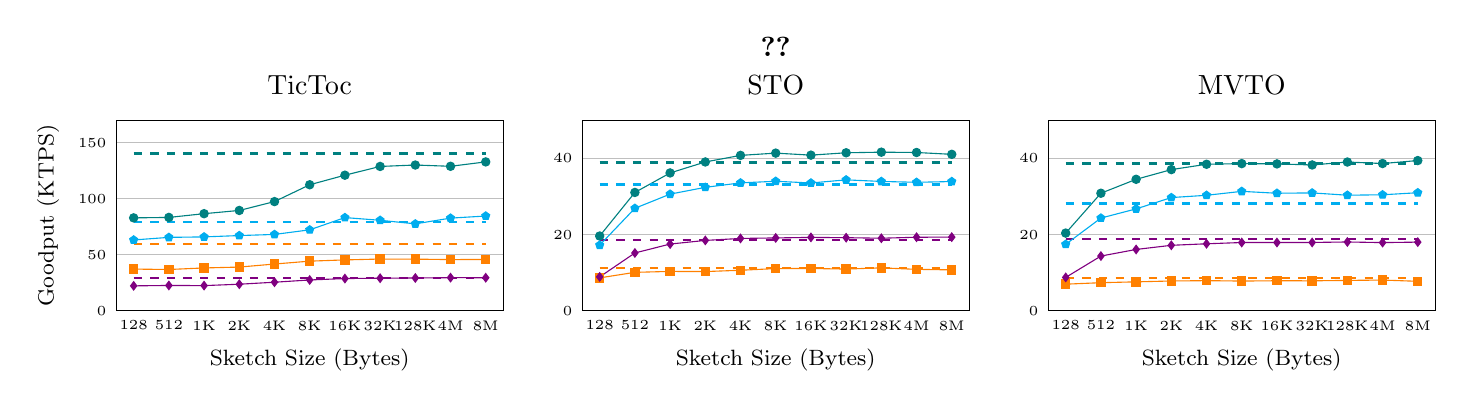
\begin{tikzpicture}
            \begin{groupplot}[group style={group size=3 by 1},
                    width=6.5cm, height=4cm,
                    major x tick style=transparent,
                    major y tick style=transparent,
                    ymajorgrids=true,
                    enlarge x limits={0.05}, % Adjust this value to reduce padding on left and right
                    xticklabel style={font=\tiny}, % Enlarges the xtick labels
                    yticklabel style={font=\tiny}, % Enlarges the xtick labels
                    label style={font=\footnotesize},
                    xlabel={Sketch Size (Bytes)},
                    symbolic x coords={128, 512, 1K, 2K, 4K, 8K, 16K, 32K, 128K, 4M, 8M},
                    xtick=data,
                    scaled y ticks=false,
                    legend columns=-1,
                    legend entries={{\ssmall Read-intensive, 673M keys, 120 threads},
                            {\ssmall Write-intensive, 673M keys, 120 threads},
                            {\ssmall Read-intensive, 673M keys, 16 threads},
                            {\ssmall Read-intensive, 67.3M keys, 120 threads}},
                    legend to name=grouplegend,
                    ymin=0,
                ]

                \nextgroupplot[title={TicToc}, ylabel={Goodput (KTPS)}, ymax=170]
                \addplot[mark=*, mark size=1.5, color=teal] %Read-intensive,673M keys,120 threads
                coordinates {
                        (128,82.9978)
                        (512,83.3859)
                        (1K,86.7366)
                        (2K,89.6129)
                        (4K,97.5232)
                        (8K,112.558)
                        (16K,121.09)
                        (32K,128.901)
                        (128K,130.175)
                        (4M,129.034)
                        (8M,132.957)
                    };
                \draw [dashed, color=teal, line width=1pt] (axis cs:128,140.330333) -- (axis cs:8M,140.330333);
                \addplot[mark=square*, mark size=1.5, color=orange] %Write-intensive,673M keys,120 threads
                coordinates {
                        (128,37.2635)
                        (512,36.9126)
                        (1K,38.2873)
                        (2K,39.0611)
                        (4K,41.783)
                        (8K,44.3566)
                        (16K,45.466)
                        (32K,46.2377)
                        (128K,46.1481)
                        (4M,45.7558)
                        (8M,45.8451)
                    };
                \draw [dashed, color=orange, line width=1pt] (axis cs:128,59.562333) -- (axis cs:8M,59.562333);
                \addplot[mark=diamond*, mark size=1.5, color=violet] %Read-intensive,673M keys,16 threads
                coordinates {
                        (128,22.2997)
                        (512,22.6541)
                        (1K,22.5158)
                        (2K,23.7622)
                        (4K,25.5448)
                        (8K,27.5555)
                        (16K,28.8266)
                        (32K,29.1491)
                        (128K,29.3334)
                        (4M,29.6163)
                        (8M,29.5459)
                    };
                \draw [dashed, color=violet, line width=1pt] (axis cs:128,29.4049) -- (axis cs:8M,29.4049);
                \addplot[mark=pentagon*, mark size=1.5, color=cyan] %Read-intensive,67.3M keys,120 threads
                coordinates {
                        (128,63.275)
                        (512,65.5834)
                        (1K,66.0073)
                        (2K,67.1957)
                        (4K,68.205)
                        (8K,72.3128)
                        (16K,83.2532)
                        (32K,80.8433)
                        (128K,77.646)
                        (4M,82.7698)
                        (8M,84.643)
                    };
                \draw [dashed, color=cyan, line width=1pt] (axis cs:128,79.3477) -- (axis cs:8M,79.3477);
                \coordinate (top) at (rel axis cs:0,1);% coordinate at top of the first plot

                \nextgroupplot[title={STO}, ymax=50]
                \addplot[mark=*, mark size=1.5, color=teal] %Read-intensive,673M keys,120 threads
                coordinates {
                        (128,19.6455)
                        (512,31.0831)
                        (1K,36.2078)
                        (2K,39.0886)
                        (4K,40.8162)
                        (8K,41.41)
                        (16K,40.8792)
                        (32K,41.5003)
                        (128K,41.6591)
                        (4M,41.5734)
                        (8M,41.0942)
                    };
                \draw [dashed, color=teal, line width=1pt] (axis cs:128,38.878867) -- (axis cs:8M,38.878867);
                \addplot[mark=square*, mark size=1.5, color=orange] %Write-intensive,673M keys,120 threads
                coordinates {
                        (128,8.65522)
                        (512,10.1074)
                        (1K,10.3501)
                        (2K,10.31)
                        (4K,10.6523)
                        (8K,11.0946)
                        (16K,11.1151)
                        (32K,10.9688)
                        (128K,11.2838)
                        (4M,10.891)
                        (8M,10.7543)
                    };
                \draw [dashed, color=orange, line width=1pt] (axis cs:128,11.258033) -- (axis cs:8M,11.258033);
                \addplot[mark=diamond*, mark size=1.5, color=violet] %Read-intensive,673M keys,16 threads
                coordinates {
                        (128,8.91054)
                        (512,15.1936)
                        (1K,17.5348)
                        (2K,18.488)
                        (4K,19.0083)
                        (8K,19.1409)
                        (16K,19.2812)
                        (32K,19.2058)
                        (128K,19.0619)
                        (4M,19.3269)
                        (8M,19.3516)
                    };
                \draw [dashed, color=violet, line width=1pt] (axis cs:128,18.6079) -- (axis cs:8M,18.6079);
                \addplot[mark=pentagon*, mark size=1.5, color=cyan] %Read-intensive,67.3M keys,120 threads
                coordinates {
                        (128,17.2532)
                        (512,26.922)
                        (1K,30.644)
                        (2K,32.4291)
                        (4K,33.5935)
                        (8K,34.0212)
                        (16K,33.5703)
                        (32K,34.3889)
                        (128K,33.9737)
                        (4M,33.7475)
                        (8M,33.9494)
                    };
                \draw [dashed, color=cyan, line width=1pt] (axis cs:128,33.0965) -- (axis cs:8M,33.0965);

                \nextgroupplot[title={MVTO}, ymax=50]
                \addplot[mark=*, mark size=1.5, color=teal] %Read-intensive,673M keys,120 threads
                coordinates {
                        (128,20.4138)
                        (512,30.8773)
                        (1K,34.5335)
                        (2K,37.081)
                        (4K,38.4838)
                        (8K,38.6555)
                        (16K,38.5799)
                        (32K,38.3015)
                        (128K,39.0719)
                        (4M,38.677)
                        (8M,39.458)
                    };
                \draw [dashed, color=teal, line width=1pt] (axis cs:128,38.669267) -- (axis cs:8M,38.669267);
                \addplot[mark=square*, mark size=1.5, color=orange] %Write-intensive,673M keys,120 threads
                coordinates {
                        (128,7.00038)
                        (512,7.38717)
                        (1K,7.61149)
                        (2K,7.83633)
                        (4K,7.92758)
                        (8K,7.81979)
                        (16K,7.89813)
                        (32K,7.87943)
                        (128K,7.99129)
                        (4M,8.07723)
                        (8M,7.75257)
                    };
                \draw [dashed, color=orange, line width=1pt] (axis cs:128,8.60338) -- (axis cs:8M,8.60338);
                \addplot[mark=diamond*, mark size=1.5, color=violet] %Read-intensive,673M keys,16 threads
                coordinates {
                        (128,8.77212)
                        (512,14.3849)
                        (1K,16.1168)
                        (2K,17.2062)
                        (4K,17.6023)
                        (8K,17.9371)
                        (16K,17.9369)
                        (32K,17.9554)
                        (128K,18.0786)
                        (4M,17.917)
                        (8M,18.0425)
                    };
                \draw [dashed, color=violet, line width=1pt] (axis cs:128,18.8555) -- (axis cs:8M,18.8555);
                \addplot[mark=pentagon*, mark size=1.5, color=cyan] %Read-intensive,67.3M keys,120 threads
                coordinates {
                        (128,17.4626)
                        (512,24.3576)
                        (1K,26.7674)
                        (2K,29.7418)
                        (4K,30.3356)
                        (8K,31.3706)
                        (16K,30.8751)
                        (32K,30.9642)
                        (128K,30.3586)
                        (4M,30.473)
                        (8M,31.0096)
                    };
                \draw [dashed, color=cyan, line width=1pt] (axis cs:128,28.0994) -- (axis cs:8M,28.0994);
                \coordinate (bot) at (rel axis cs:1,0);% coordinate at bottom of the last plot
            \end{groupplot}
            \coordinate (c) at ($(top)!.5!(bot)$);
            \node[above] at (c |- current bounding box.north) {\ref{grouplegend}};
        \end{tikzpicture}
    }
    \caption[Factor-analysis of the sketch size]{The goodput of TicToc, STO, and MVTO for high-contended YCSB
        workloads with varying sketch sizes. We configure workloads by operations
        proportion (Read-intensive vs. Write-intensive), the database size (containing
        673M vs. 67.3M keys), and the concurrency level (120 vs 16 threads). The dashed
        lines represent the goodputs of the Memory variant for each configuration.}
    \label{fig:sketch_size}
\end{figure}



\subsection{Sketch Size}


We conduct a factor-analysis of the sketch size of \sketchname for TicToc, STO,
and MVTO. \Cref{fig:sketch_size} presents the goodput for the high-contended
YCSB workloads as the sketch size increases. We vary workload type
(read-intensive vs. write-intensive), the number of worker threads varying the
amount of data updating the sketch, and the database size determined by the
number of keys in the database, representing the key range of workloads.

The main takeaway from these experiments is that regardless of the setting, the
sketch can be at most a few KiB, which is less than 1\% of the database size, to
avoid being a limiting factor since the goodput is similar to that of their
memory counterparts.




\section{Summary}
\label{sec:summary}


In this chapter we introduced \emph{approximate timestamp storage}, a
novel timestamp storage system that enables timestamp-based CC
mechanisms to operate efficiently in modern on-disk key-value stores.
Approximate timestamp storage provides guarantees we identified to be
sufficient for preserving the correctness of the timestamp-based CC
mechanisms we studied, while being extremely memory efficient. We
presented the design of an approximate timestamp storage system,
\sketchname, and implemented two of its variants, \fsketchname and
\psketchname. We integrated \sketchname with three timestamp-based CC
protocols--STO, MVTO, and TicToc. Our evaluation shows superior
performance across various workloads using our \sketchname approach.
Notably, TicToc with \psketchname achieves up to 11$\times$ better
performance than traditional 2PL and OCC approaches, and up to
27$\times$ improvement over disk-based timestamp storage. \sketchname
unlocks the ability to adapt existing CC techniques and paves the way
for innovative CC mechanisms in future disk-based key-value stores.

We believe \sketchname is broadly applicable across a variety of
domains, although the performance benefits may vary based on other
overheads in the system.  For example, our approach could benefit
distributed systems by improving local node performance. In a
shared-nothing architecture, a per-partition \sketchname instance
could manage timestamps for its corresponding keys, providing the
same local memory efficiency and reduced disk I/O demonstrated in
our work.  In distributed systems or in systems based on older data
structures, such as B-trees, other performance bottlenecks will
obviously reduce the impact of an optimized concurrency-control
mechanism.  However, extensive research has focused on optimizing
these aspects through techniques like reducing network round-trips
and improving global timestamp synchronization. As those orthogonal
optimizations are applied, the local performance improvements
provided by \sketchname would become even more promising for overall
system throughput.

\chapter{Evaluating \sketchname Across the Storage Spectrum}
\label{chapter:four}
Storage technologies in production environments span several orders of magnitude
in performance---from traditional hard disk drives (HDDs) with millisecond 
latencies to emerging byte-addressable storage like CXL-based flash approaching 
DRAM-like speeds. Since \sketchname enables modern timestamp-based concurrency 
control for disk-based key-value stores, evaluating its effectiveness across this 
performance spectrum is critical for understanding both current deployment 
opportunities and future applicability as storage technologies continue to evolve.

This chapter presents a comprehensive evaluation across slow storage (SATA SSD and 
HDD) in Section~\ref{sec:slow-storage} and fast storage (emulated CXL-based flash) 
in Section~\ref{sec:fast-storage} to reveal how \sketchname's benefits and 
trade-offs evolve with storage characteristics. Our analysis demonstrates that 
\sketchname remains effective across this wide range, though the nature of its 
advantages changes fundamentally as storage performance improves.


\section{Slow Storage}\label{sec:slow-storage}

We begin our evaluation with slow storage scenarios, which represent traditional
disk-based systems where storage latency significantly impacts transaction
processing performance. On slow storage, disk I/O becomes the dominant bottleneck,
making the elimination of timestamp disk accesses provided by \sketchname 
particularly valuable. These results demonstrate how \sketchname performs under
challenging storage conditions and reveal its effectiveness when storage 
characteristics fundamentally limit transaction throughput.

We use the same workloads and evaluation methods as in Section~\ref{sec:eval}.
For slow storage setups, we run experiments using both SATA SSD and HDD. The
SATA SSD experiments are run on the same type of machine as the NVMe SSD tests,
with only the storage hardware changed. However, for the HDD tests, we use a
different machine because CloudLab does not offer machines with HDDs. Using SATA
SSD allows us to compare results fairly with NVMe SSD and other faster storage.
In contrast, the HDD experiments show how \sketchname performs on a real hard
disk, helping us understand its behavior in truly slow storage situations.


\subsection{SATA SSD}

\subsubsection{YCSB Small-Transaction Workloads}

Figure~\ref{fig:ycsb:slow_ssd} presents the goodput of all our timestamp-based
concurrency control (CC) variants on four YCSB small-transaction workloads using
slow SSD storage. The patterns in the results are similar to those shown in
Section~\ref{sec:eval} for NVMe SSD. The \sketchname variants regularly achieve
goodput very close to the Memory setup, which shows that they remain effective
even when storage is slower.

In read-intensive workloads, the \sketchname variants (\fsketchname and
\psketchname) almost match the goodput of the Memory setup. They improve goodput
by as much as 39\% compared to the Disk variant when contention is high, and up
to 23\% better in medium-contention situations. The TicToc-\psketchname setup in
particular improves goodput by 65\% over 2PL and by 19\% over KR-OCC in
workloads with high contention.

For write-intensive workloads, the difference in goodput becomes even greater.
Here, the \sketchname variants (\fsketchname and \psketchname) again produce
goodput close to the Memory variant. In high-contention cases, they boost
goodput by up to 569\% over the Disk variant, and by up to 119\% when contention
is medium. The TicToc-\psketchname configuration shows especially strong
results, delivering 589\% and 152\% higher goodput than 2PL and KR-OCC,
respectively, for high-contention workloads.

TicToc is a highly concurrent CC method that uses timestamps. When combined with
\sketchname, TicToc achieves the best performance in all workloads. This is
because \sketchname removes the need to frequently access timestamps on disk,
which lessens storage delays. \sketchname is especially helpful for
write-intensive, high-contention workloads, because these workloads consist of
quick operations enabled by SplinterDB's fast write speed and high cache hit
rate even though storage is slow.



\begin{figure}[!t]
    \centering
    \resizebox{\textwidth}{!}{%
        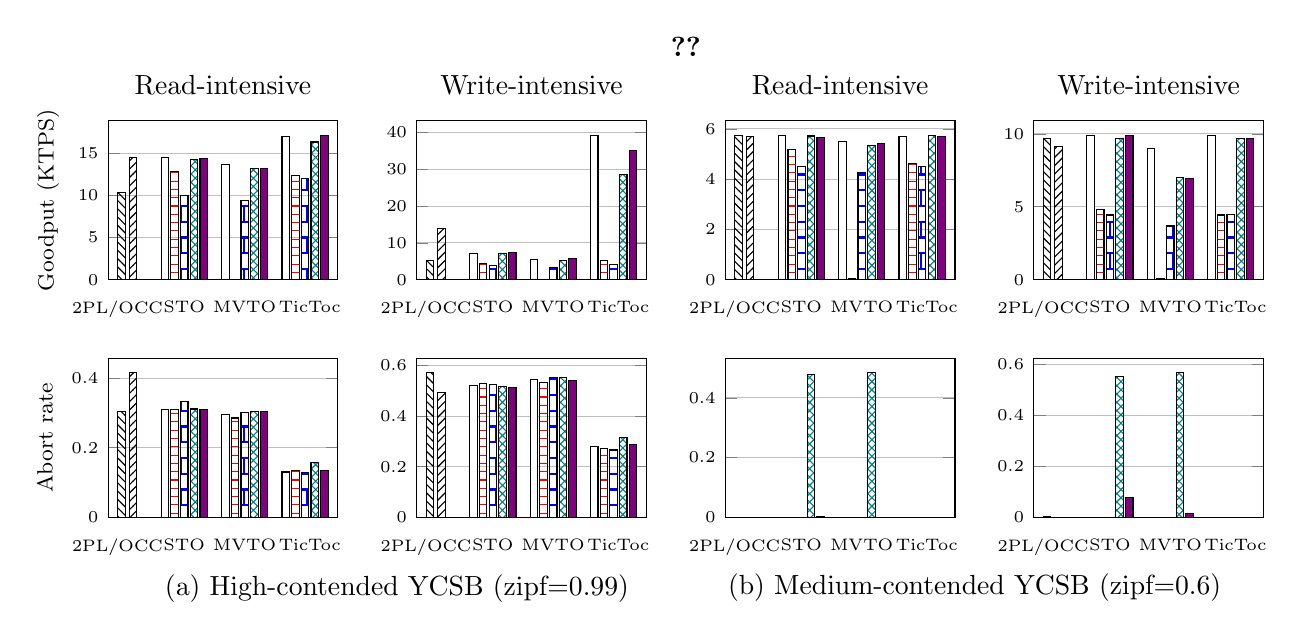
\begin{tikzpicture}
            \begin{groupplot}[group style={group size=4 by 2,
                            /pgf/bar width=2.7pt},
                    height = 3.6cm,
                    width = 4.5cm,
                    ybar= 2*\pgflinewidth,
                    xtick={-1, 0.425, 1.7125, 3.1},
                    xticklabels={2PL/OCC, STO, MVTO, TicToc},
                    ymajorgrids=true,
                    enlarge x limits = 0.2,
                    legend columns=-1,
                    legend entries={{\ssmall Memory (Idealized)}, {\ssmall Disk}, {\ssmall Disk-Cache}, {\ssmall \fsketchname},  {\ssmall \psketchname}},
                    area legend,
                    legend to name=grouplegend,
                ]

                % graph [1,1] high
                \nextgroupplot[title={Read-intensive},YCSBThroughputBarChartPlot, ylabel={Goodput (KTPS)}]
                \addplot[2PL-BarStyle, forget plot] coordinates {(-0.5, 10.364933)};
                \addplot[KR-OCC-BarStyle, forget plot] coordinates {(-0.26, 14.441267)};
                \addplot[Memory-BarStyle] coordinates {(0.425, 14.425833) (1.7125, 13.695567) (3, 16.9643)};
                \addplot[Disk-BarStyle] coordinates {(0.425, 12.791433) (1.7125, 0.05428) (3, 12.298733)};
                \addplot[Disk-Cache-BarStyle] coordinates {(0.425, 9.92869) (1.7125, 9.340693) (3, 11.959133)};
                \addplot[Counter-Lazy-BarStyle] coordinates {(0.425, 14.190467) (1.7125, 13.124533) (3, 16.308867)};
                \addplot[FPSketch-BarStyle] coordinates {(0.425, 14.404033) (1.7125, 13.169733) (3, 17.120333)};
                \coordinate (top) at (rel axis cs:0,1);% coordinate at top of the first plot

                % graph [1,3] high
                \nextgroupplot[title={Write-intensive}, YCSBThroughputBarChartPlot]
                \addplot[2PL-BarStyle, forget plot] coordinates {(-0.5, 5.088527)};
                \addplot[KR-OCC-BarStyle, forget plot] coordinates {(-0.26, 13.9281)};
                \addplot[Memory-BarStyle] coordinates {(0.425, 7.07645) (1.7125, 5.59584) (3, 39.2637)};
                \addplot[Disk-BarStyle] coordinates {(0.425, 4.271767) (1.7125, 0.05016) (3, 5.239043)};
                \addplot[Disk-Cache-BarStyle] coordinates {(0.425, 3.879563) (1.7125, 3.21073) (3, 4.171167)};
                \addplot[Counter-Lazy-BarStyle] coordinates {(0.425, 7.14758) (1.7125, 5.09302) (3, 28.504433)};
                \addplot[FPSketch-BarStyle] coordinates {(0.425, 7.34722) (1.7125, 5.753657) (3, 35.0623)};

                % graph [1,1] medium
                \nextgroupplot[title={Read-intensive},YCSBThroughputBarChartPlot]
                \addplot[2PL-BarStyle, forget plot] coordinates {(-0.5, 5.74492)};
                \addplot[KR-OCC-BarStyle, forget plot] coordinates {(-0.26, 5.701743)};
                \addplot[Memory-BarStyle] coordinates {(0.425, 5.749967) (1.7125, 5.49676) (3, 5.710213)};
                \addplot[Disk-BarStyle] coordinates {(0.425, 5.171957) (1.7125, 0.046666) (3, 4.639907)};
                \addplot[Disk-Cache-BarStyle] coordinates {(0.425, 4.499663) (1.7125, 4.262087) (3, 4.50323)};
                \addplot[Counter-Lazy-BarStyle] coordinates {(0.425, 5.717253) (1.7125, 5.33784) (3, 5.73195)};
                \addplot[FPSketch-BarStyle] coordinates {(0.425, 5.67032) (1.7125, 5.405587) (3, 5.707593)};


                % graph [1,3] medium
                \nextgroupplot[title={Write-intensive},YCSBThroughputBarChartPlot]
                \addplot[2PL-BarStyle, forget plot] coordinates {(-0.5, 9.648553)};
                \addplot[KR-OCC-BarStyle, forget plot] coordinates {(-0.26, 9.156227)};
                \addplot[Memory-BarStyle] coordinates {(0.425, 9.86155) (1.7125, 8.966833) (3, 9.90628)};
                \addplot[Disk-BarStyle] coordinates {(0.425, 4.785737) (1.7125, 0.044312) (3, 4.43323)};
                \addplot[Disk-Cache-BarStyle] coordinates {(0.425, 4.431213) (1.7125, 3.680533) (3, 4.480477)};
                \addplot[Counter-Lazy-BarStyle] coordinates {(0.425, 9.65755) (1.7125, 6.98781) (3, 9.650477)};
                \addplot[FPSketch-BarStyle] coordinates {(0.425, 9.859053) (1.7125, 6.96129) (3, 9.68747)};
                \coordinate (bot) at (rel axis cs:1,0);% coordinate at bottom of the last plot

                % graph [1,2] read intensive
                \nextgroupplot[AbortRateBarChartPlot, ylabel={Abort rate}]
                \addplot[2PL-BarStyle, forget plot] coordinates {(-0.5, 0.304596)};
                \addplot[KR-OCC-BarStyle, forget plot] coordinates {(-0.26, 0.415079)};
                \addplot[Memory-BarStyle] coordinates {(0.425, 0.310117) (1.7125, 0.294705) (3, 0.13013)};
                \addplot[Disk-BarStyle] coordinates {(0.425, 0.309437) (1.7125, 0.285392) (3, 0.134926)};
                \addplot[Disk-Cache-BarStyle] coordinates {(0.425, 0.332255) (1.7125, 0.300908) (3, 0.130042)};
                \addplot[Counter-Lazy-BarStyle] coordinates {(0.425, 0.311321) (1.7125, 0.302894) (3, 0.157114)};
                \addplot[FPSketch-BarStyle] coordinates {(0.425, 0.308572) (1.7125, 0.304875) (3, 0.134233)};

                % graph [1,4] write intensive
                \nextgroupplot[AbortRateBarChartPlot]
                \addplot[2PL-BarStyle, forget plot] coordinates {(-0.5, 0.571121)};
                \addplot[KR-OCC-BarStyle, forget plot] coordinates {(-0.26, 0.495017)};
                \addplot[Memory-BarStyle] coordinates {(0.425, 0.520538) (1.7125, 0.54321) (3, 0.280598)};
                \addplot[Disk-BarStyle] coordinates {(0.425, 0.528094) (1.7125, 0.533668) (3, 0.272687)};
                \addplot[Disk-Cache-BarStyle] coordinates {(0.425, 0.523497) (1.7125, 0.551743) (3, 0.266006)};
                \addplot[Counter-Lazy-BarStyle] coordinates {(0.425, 0.51712) (1.7125, 0.551956) (3, 0.316003)};
                \addplot[FPSketch-BarStyle] coordinates {(0.425, 0.511699) (1.7125, 0.540079) (3, 0.289621)};

                % graph [1,2]
                \nextgroupplot[AbortRateBarChartPlot]
                \addplot[2PL-BarStyle, forget plot] coordinates {(-0.5, 0.000554)};
                \addplot[KR-OCC-BarStyle, forget plot] coordinates {(-0.26, 0.000204)};
                \addplot[Memory-BarStyle] coordinates {(0.425, 0.000093) (1.7125, 0.000098) (3, 0.000032)};
                \addplot[Disk-BarStyle] coordinates {(0.425, 0.000085) (1.7125, 0.000089) (3, 0.000037)};
                \addplot[Disk-Cache-BarStyle] coordinates {(0.425, 0.000089) (1.7125, 0.000077) (3, 0.000033)};
                \addplot[Counter-Lazy-BarStyle] coordinates {(0.425, 0.479464) (1.7125, 0.483513) (3, 0.000094)};
                \addplot[FPSketch-BarStyle] coordinates {(0.425, 0.001726) (1.7125, 0.000607) (3, 0.000087)};

                % graph [1,4]
                \nextgroupplot[AbortRateBarChartPlot]
                \addplot[2PL-BarStyle, forget plot] coordinates {(-0.5, 0.004177)};
                \addplot[KR-OCC-BarStyle, forget plot] coordinates {(-0.26, 0.000907)};
                \addplot[Memory-BarStyle] coordinates {(0.425, 0.000498) (1.7125, 0.000473) (3, 0.000191)};
                \addplot[Disk-BarStyle] coordinates {(0.425, 0.000566) (1.7125, 0.000276) (3, 0.000297)};
                \addplot[Disk-Cache-BarStyle] coordinates {(0.425, 0.000493) (1.7125, 0.000509) (3, 0.000351)};
                \addplot[Counter-Lazy-BarStyle] coordinates {(0.425, 0.553703) (1.7125, 0.566425) (3, 0.000453)};
                \addplot[FPSketch-BarStyle] coordinates {(0.425, 0.077443) (1.7125, 0.01577) (3, 0.000418)};

            \end{groupplot}
            \coordinate (c) at ($(top)!.5!(bot)$);
            \coordinate (cc1) at ($(top)!.25!(bot)$);
            \coordinate (cc2) at ($(top)!.75!(bot)$);

            \node[above] at (c |- current bounding box.north) {\ref{grouplegend}};
            \node[below] at (cc1 |- current bounding box.south) {(a) High-contended YCSB (zipf=0.99)};
            \node[above] at (cc2 |- current bounding box.south) {(b) Medium-contended YCSB (zipf=0.6)};
        \end{tikzpicture}
    } \caption[YCSB small-transaction workloads results on slow SSD]{YCSB
    small-transaction workloads results with 120 processing threads on slow SSD.
    In write-intensive workloads, each transaction performs 8 reads and 8
    writes. In read-intensive workloads, each transaction performs 15 reads and
    1 write. Note that, in the medium-contended workload, several variants have
    abort rates very close to 0.}
    \label{fig:ycsb:slow_ssd}
\end{figure}

\subsubsection{YCSB Mixed-Transaction Workloads}

\begin{figure}[!t]
    \centering
    \resizebox{\textwidth}{!}{%
        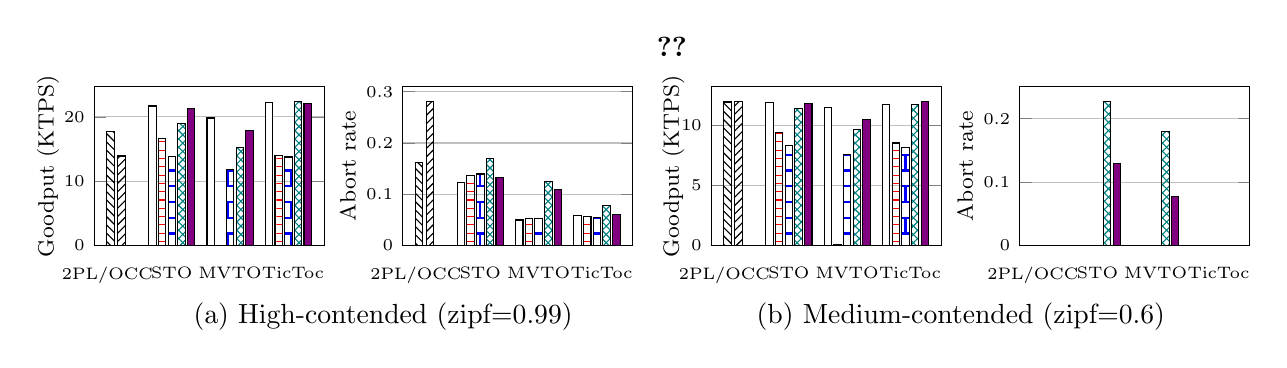
\begin{tikzpicture}
            \begin{groupplot}[group style={group size=4 by 1,
                            /pgf/bar width=2.7pt},
                    height = 3.6cm,
                    width = 4.5cm,
                    ybar= 2*\pgflinewidth,
                    xtick={-1, 0.425, 1.7125, 3.1},
                    xticklabels={2PL/OCC, STO, MVTO, TicToc},
                    ymajorgrids=true,
                    enlarge x limits = 0.225,
                    legend columns=-1,
                    legend entries={{\ssmall Memory (Idealized)}, {\ssmall Disk}, {\ssmall Disk-Cache}, {\ssmall \fsketchname},  {\ssmall \psketchname}},
                    area legend,
                    legend to name=grouplegend,
                ]

                % graph [1,1] high
                \nextgroupplot[YCSBThroughputBarChartPlot, ylabel={Goodput (KTPS)}, ylabel style={yshift=-5pt}]
                \addplot[2PL-BarStyle, forget plot] coordinates {(-0.5, 17.7908)};
                \addplot[KR-OCC-BarStyle, forget plot] coordinates {(-0.26, 13.9216)};
                \addplot[Memory-BarStyle] coordinates {(0.425, 21.6929) (1.7125, 19.823333) (3, 22.264467)};
                \addplot[Disk-BarStyle] coordinates {(0.425, 16.7041) (1.7125, 0.071738) (3, 13.9898)};
                \addplot[Disk-Cache-BarStyle] coordinates {(0.425, 13.890367) (1.7125, 11.8303) (3, 13.760167)};
                \addplot[Counter-Lazy-BarStyle] coordinates {(0.425, 18.941667) (1.7125, 15.2963) (3, 22.4423)};
                \addplot[FPSketch-BarStyle] coordinates {(0.425, 21.315967) (1.7125, 17.8994) (3, 22.084967)};
                \coordinate (top) at (rel axis cs:0,1);% coordinate at top of the first plot

                % graph [2,1] abort rate
                \nextgroupplot[AbortRateBarChartPlot, ylabel={Abort rate}, ylabel style={yshift=-3pt}]
                \addplot[2PL-BarStyle, forget plot] coordinates {(-0.5, 0.162546)};
                \addplot[KR-OCC-BarStyle, forget plot] coordinates {(-0.26, 0.281549)};
                \addplot[Memory-BarStyle] coordinates {(0.425, 0.123194) (1.7125, 0.050042) (3, 0.058888)};
                \addplot[Disk-BarStyle] coordinates {(0.425, 0.1363) (1.7125, 0.052943) (3, 0.057104)};
                \addplot[Disk-Cache-BarStyle] coordinates {(0.425, 0.139533) (1.7125, 0.052058) (3, 0.05523)};
                \addplot[Counter-Lazy-BarStyle] coordinates {(0.425, 0.170173) (1.7125, 0.125589) (3, 0.078445)};
                \addplot[FPSketch-BarStyle] coordinates {(0.425, 0.13226) (1.7125, 0.108899) (3, 0.06144)};

                % graph [3,1] medium
                \nextgroupplot[YCSBThroughputBarChartPlot, ylabel={Goodput (KTPS)}, ylabel style={yshift=-8pt}]
                \addplot[2PL-BarStyle, forget plot] coordinates {(-0.5, 11.919633)};
                \addplot[KR-OCC-BarStyle, forget plot] coordinates {(-0.26, 11.989233)};
                \addplot[Memory-BarStyle] coordinates {(0.425, 11.891433) (1.7125, 11.464433) (3, 11.743967)};
                \addplot[Disk-BarStyle] coordinates {(0.425, 9.385673) (1.7125, 0.082369) (3, 8.519537)};
                \addplot[Disk-Cache-BarStyle] coordinates {(0.425, 8.327213) (1.7125, 7.538987) (3, 8.14708)};
                \addplot[Counter-Lazy-BarStyle] coordinates {(0.425, 11.3492) (1.7125, 9.616147) (3, 11.706867)};
                \addplot[FPSketch-BarStyle] coordinates {(0.425, 11.7846) (1.7125, 10.483733) (3, 11.955533)};

                % graph [4,1] medium abort rate
                \nextgroupplot[AbortRateBarChartPlot, ylabel={Abort rate}, ylabel style={yshift=-3pt}]
                \addplot[2PL-BarStyle, forget plot] coordinates {(-0.5, 0.000607)};
                \addplot[KR-OCC-BarStyle, forget plot] coordinates {(-0.26, 0.000509)};
                \addplot[Memory-BarStyle] coordinates {(0.425, 0.00026) (1.7125, 0.000032) (3, 0.000075)};
                \addplot[Disk-BarStyle] coordinates {(0.425, 0.000203) (1.7125, 0.000052) (3, 0.000076)};
                \addplot[Disk-Cache-BarStyle] coordinates {(0.425, 0.000178) (1.7125, 0.000175) (3, 0.000064)};
                \addplot[Counter-Lazy-BarStyle] coordinates {(0.425, 0.227664) (1.7125, 0.180463) (3, 0.000257)};
                \addplot[FPSketch-BarStyle] coordinates {(0.425, 0.128828) (1.7125, 0.078013) (3, 0.000214)};
                \coordinate (bot) at (rel axis cs:1,0);% coordinate at bottom of the last plot

            \end{groupplot}
            \coordinate (c) at ($(top)!.5!(bot)$);
            \coordinate (cc1) at ($(top)!.25!(bot)$);
            \coordinate (cc2) at ($(top)!.75!(bot)$);

            \node[above] at (c |- current bounding box.north) {\ref{grouplegend}};
            \node[below] at (cc1 |- current bounding box.south) {(a) High-contended (zipf=0.99)};
            \node[above] at (cc2 |- current bounding box.south) {(b) Medium-contended (zipf=0.6)};
        \end{tikzpicture}
    } \caption[YCSB mixed-transaction workloads results on slow SSD]{YCSB
    mixed-transaction workloads results with 120 processing threads on slow SSD.
    80\% of transactions perform 2 reads and 2 writes, and 20\% of transactions
    perform 28 reads. Note that, in the medium-contended workload, several
    variants have abort rates very close to 0.}
    \label{fig:ycsb:mixed:slow_ssd}
\end{figure}


In \Cref{fig:ycsb:mixed:slow_ssd}, both \sketchname variants show strong
performance in mixed-transaction settings on slow SSD. In high-contention
scenarios, \sketchname offers up to 60\% higher goodput than the Disk variants.
It also outperforms 2PL and KR-OCC, with goodput increases of up to 24\% and
59\%, respectively.

Under medium contention, the goodputs of these systems are mainly limited by
slow disk access. Unlike our evaluation with NVMe SSDs described in
\Cref{sec:eval}, the concurrency control method has little effect on overall
goodput. However, since the Disk variants must fetch timestamps from the disk,
there is extra overhead, resulting in lower goodput. \sketchname avoids this
disk overhead and can improve goodput by up to 40\%.




\subsubsection{YCSB Long-Transaction Workloads}


\begin{figure}[!t]
    \centering
    \resizebox{.75\textwidth}{!}{%
        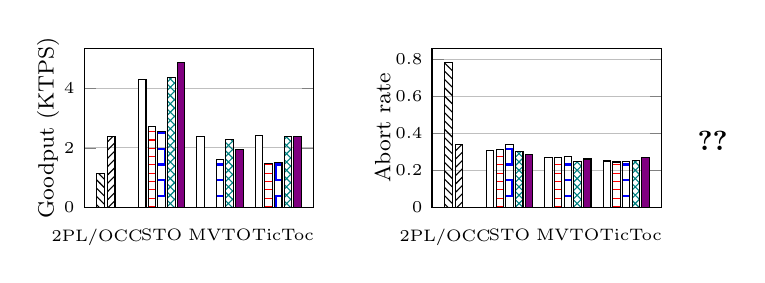
\begin{tikzpicture}
            \begin{groupplot}[group style={
                            group size=2 by 1,
                            horizontal sep=1.5cm,
                            /pgf/bar width=2.7pt
                        },
                    height = 3.6cm,
                    width = 4.5cm,
                    ybar= 2*\pgflinewidth,
                    xtick={-1, 0.425, 1.7125, 3.1},
                    xticklabels={2PL/OCC, STO, MVTO, TicToc},
                    ymajorgrids=true,
                    enlarge x limits = 0.225,
                    legend columns=1,
                    legend entries={{\ssmall Memory (Idealized)}, {\ssmall Disk}, {\ssmall Disk-Cache}, {\ssmall \fsketchname},  {\ssmall \psketchname}},
                    area legend,
                    legend to name=grouplegend,
                ]

                % graph [1,1] high
                \nextgroupplot[YCSBThroughputBarChartPlot, ylabel={Goodput (KTPS)}, ylabel style={yshift=-5pt}]
                \addplot[2PL-BarStyle, forget plot] coordinates {(-0.5, 1.132117)};
                \addplot[KR-OCC-BarStyle, forget plot] coordinates {(-0.26, 2.381903)};
                \addplot[Memory-BarStyle] coordinates {(0.425, 4.298397) (1.7125, 2.3857) (3, 2.398567)};
                \addplot[Disk-BarStyle] coordinates {(0.425, 2.726483) (1.7125, 0.006448) (3, 1.47637)};
                \addplot[Disk-Cache-BarStyle] coordinates {(0.425, 2.55686) (1.7125, 1.613997) (3, 1.495053)};
                \addplot[Counter-Lazy-BarStyle] coordinates {(0.425, 4.369143) (1.7125, 2.26709) (3, 2.393783)};
                \addplot[FPSketch-BarStyle] coordinates {(0.425, 4.84888) (1.7125, 1.949793) (3, 2.39416)};
                \coordinate (top) at (rel axis cs:0,1);% coordinate at top of the first plot

                % graph [1,2] abort rate
                \nextgroupplot[AbortRateBarChartPlot, ylabel={Abort rate}, ylabel style={yshift=-5pt}]
                \addplot[2PL-BarStyle, forget plot] coordinates {(-0.5, 0.780498)};
                \addplot[KR-OCC-BarStyle, forget plot] coordinates {(-0.26, 0.338777)}; 
                \addplot[Memory-BarStyle] coordinates {(0.425, 0.306208) (1.7125, 0.271251) (3, 0.250567)};
                \addplot[Disk-BarStyle] coordinates {(0.425, 0.311134) (1.7125, 0.268125) (3, 0.24539)};
                \addplot[Disk-Cache-BarStyle] coordinates {(0.425, 0.340524) (1.7125, 0.275897) (3, 0.249158)};
                \addplot[Counter-Lazy-BarStyle] coordinates {(0.425, 0.30175) (1.7125, 0.249261) (3, 0.25168)};
                \addplot[FPSketch-BarStyle] coordinates {(0.425, 0.287686) (1.7125, 0.261718) (3, 0.268675)};
                \coordinate (bot) at (rel axis cs:1,0);% coordinate at bottom of the last plot

            \end{groupplot}
            \coordinate (c) at ($(top)!.5!(bot)$);

            \node[right=4cm] at (c |- current bounding box.east) {\ref{grouplegend}};
        \end{tikzpicture}
    }
    \caption[YCSB long-transaction workloads results on slow SSD]{YCSB long-transaction workloads results with 120 processing threads on slow SSD. 5\% of transactions perform 1000 reads and the rest of transactions perform 8 writes and 8 reads. The distribution is Zipfian with 0.9.}
    \label{fig:ycsb:long:slow_ssd}
\end{figure}


\Cref{fig:ycsb:long:slow_ssd} presents the goodput results for the
long-transaction workload on slow SSD. The main pattern is similar to previous
results: the \sketchname variants achieve higher goodput than their Disk
versions and 2PL/KR-OCC. Because the disk is slow, long transactions run more
slowly and the differences between each method are smaller than with the faster
NVMe SSD shown in \Cref{fig:ycsb:long}. Still, although \sketchname is not as
effective as with NVMe SSD, it continues to deliver the best performance among
all tested protocols.




\subsubsection{TPC-C Workloads}


\begin{figure*}[!t]
    \centering
    \resizebox{\textwidth}{!}{%
        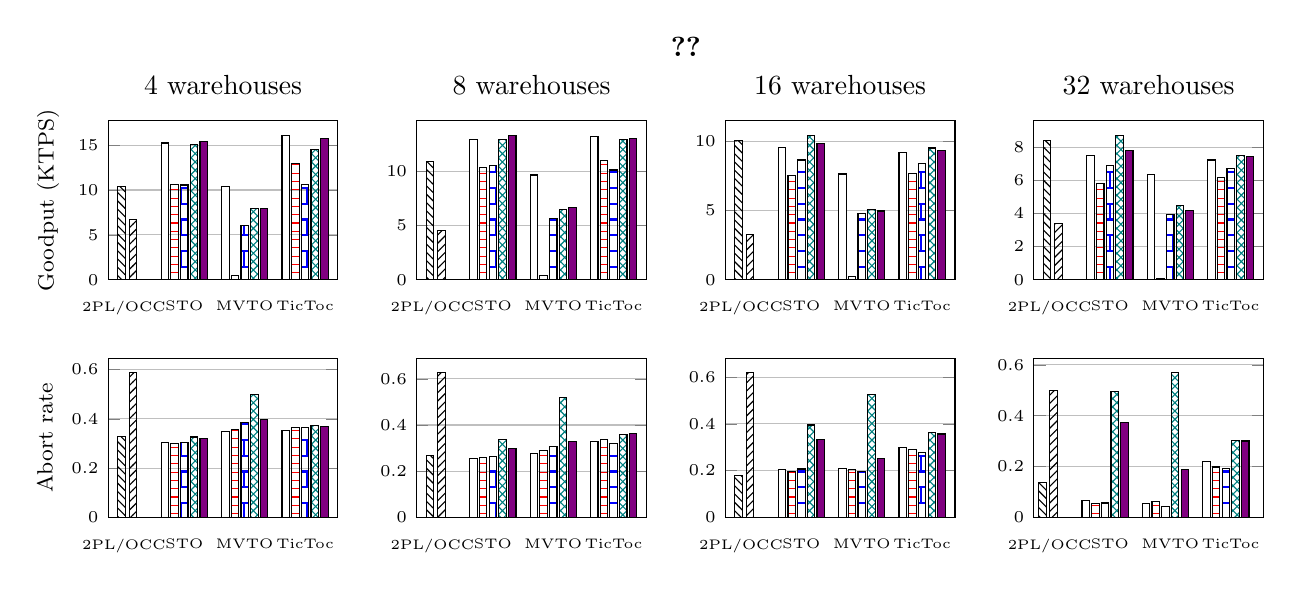
\begin{tikzpicture}
            \begin{groupplot}[group style={group size=4 by 2,
                            /pgf/bar width=2.7pt},
                    height = 3.6cm,
                    width = 4.5cm,
                    ybar= 2*\pgflinewidth,
                    xtick={-0.8625, 0.425, 1.7125, 3},
                    xticklabels={2PL/OCC, STO, MVTO, TicToc},
                    xticklabel style={font=\tiny},
                    ymajorgrids=true,
                    enlarge x limits = 0.2,
                    legend columns=-1,
                    legend entries={{\ssmall Memory (Idealized)}, {\ssmall Disk}, {\ssmall Disk-Cache}, {\ssmall \fsketchname},  {\ssmall \psketchname}},
                    area legend,
                    legend to name=grouplegend,
                ]

                % graph [1,1]
                \nextgroupplot[title={4 warehouses},YCSBThroughputBarChartPlot, ylabel={Goodput (KTPS)}]
                \addplot[2PL-BarStyle, forget plot] coordinates {(-0.5, 10.435867)};
                \addplot[KR-OCC-BarStyle, forget plot] coordinates {(-0.26, 6.705303)};
                \addplot[Memory-BarStyle] coordinates {(0.425, 15.243133) (1.7125, 10.439267) (3, 16.118167)};
                \addplot[Disk-BarStyle] coordinates {(0.425, 10.630633) (1.7125, 0.487886) (3, 12.915967)};
                \addplot[Disk-Cache-BarStyle] coordinates {(0.425, 10.555533) (1.7125, 6.000767) (3, 10.588833)};
                \addplot[Counter-Lazy-BarStyle] coordinates {(0.425, 15.047167) (1.7125, 7.931357) (3, 14.545967)};
                \addplot[FPSketch-BarStyle] coordinates {(0.425, 15.4038) (1.7125, 7.893797) (3, 15.6993)};
                \coordinate (top) at (rel axis cs:0,1);% coordinate at top of the first plot

                % graph [1,2]
                \nextgroupplot[title={8 warehouses}, YCSBThroughputBarChartPlot]
                \addplot[2PL-BarStyle, forget plot] coordinates {(-0.5, 10.954033)};
                \addplot[KR-OCC-BarStyle, forget plot] coordinates {(-0.26, 4.538743)};
                \addplot[Memory-BarStyle] coordinates {(0.425, 12.9659) (1.7125, 9.66877) (3, 13.214967)};
                \addplot[Disk-BarStyle] coordinates {(0.425, 10.404567) (1.7125, 0.370496) (3, 11.023467)};
                \addplot[Disk-Cache-BarStyle] coordinates {(0.425, 10.5734) (1.7125, 5.628667) (3, 10.133817)};
                \addplot[Counter-Lazy-BarStyle] coordinates {(0.425, 12.979) (1.7125, 6.524537) (3, 12.9708)};
                \addplot[FPSketch-BarStyle] coordinates {(0.425, 13.353233) (1.7125, 6.707457) (3, 13.025)};

                % graph [1,3]
                \nextgroupplot[title={16 warehouses},YCSBThroughputBarChartPlot]
                \addplot[2PL-BarStyle, forget plot] coordinates {(-0.5, 10.092567)};
                \addplot[KR-OCC-BarStyle, forget plot] coordinates {(-0.26, 3.257557)};
                \addplot[Memory-BarStyle] coordinates {(0.425, 9.537317) (1.7125, 7.649797) (3, 9.185967)};
                \addplot[Disk-BarStyle] coordinates {(0.425, 7.545187) (1.7125, 0.224447) (3, 7.702217)};
                \addplot[Disk-Cache-BarStyle] coordinates {(0.425, 8.662643) (1.7125, 4.814237) (3, 8.409643)};
                \addplot[Counter-Lazy-BarStyle] coordinates {(0.425, 10.459933) (1.7125, 5.09145) (3, 9.528323)};
                \addplot[FPSketch-BarStyle] coordinates {(0.425, 9.873883) (1.7125, 4.969443) (3, 9.350587)};


                % graph [1,4] 32wh
                \nextgroupplot[title={32 warehouses},YCSBThroughputBarChartPlot]
                \addplot[2PL-BarStyle, forget plot] coordinates {(-0.5, 8.402127)};
                \addplot[KR-OCC-BarStyle, forget plot] coordinates {(-0.26, 3.368457)};
                \addplot[Memory-BarStyle] coordinates {(0.425, 7.48262) (1.7125, 6.326153) (3, 7.225083)};
                \addplot[Disk-BarStyle] coordinates {(0.425, 5.781087) (1.7125, 0.077289) (3, 6.190753)};
                \addplot[Disk-Cache-BarStyle] coordinates {(0.425, 6.90269) (1.7125, 3.958337) (3, 6.694893)};
                \addplot[Counter-Lazy-BarStyle] coordinates {(0.425, 8.722823) (1.7125, 4.49392) (3, 7.51293)};
                \addplot[FPSketch-BarStyle] coordinates {(0.425, 7.79229) (1.7125, 4.189127) (3, 7.45213)};

                \coordinate (bot) at (rel axis cs:1,0);% coordinate at bottom of the last plot

                % graph [2,1] 4 wh
                \nextgroupplot[AbortRateBarChartPlot, ylabel={Abort rate}]
                \addplot[2PL-BarStyle, forget plot] coordinates {(-0.5, 0.329391)};
                \addplot[KR-OCC-BarStyle, forget plot] coordinates {(-0.26, 0.586844)};
                \addplot[Memory-BarStyle] coordinates {(0.425, 0.305108) (1.7125, 0.348413) (3, 0.351015)};
                \addplot[Disk-BarStyle] coordinates {(0.425, 0.301385) (1.7125, 0.356276) (3, 0.364606)};
                \addplot[Disk-Cache-BarStyle] coordinates {(0.425, 0.302807) (1.7125, 0.385476) (3, 0.366083)};
                \addplot[Counter-Lazy-BarStyle] coordinates {(0.425, 0.326195) (1.7125, 0.499632) (3, 0.372108)};
                \addplot[FPSketch-BarStyle] coordinates {(0.425, 0.321034) (1.7125, 0.398993) (3, 0.370333)};

                % graph [2,2] 8 wh
                \nextgroupplot[AbortRateBarChartPlot]
                \addplot[2PL-BarStyle, forget plot] coordinates {(-0.5, 0.267192)};
                \addplot[KR-OCC-BarStyle, forget plot] coordinates {(-0.26, 0.626045)};
                \addplot[Memory-BarStyle] coordinates {(0.425, 0.254501) (1.7125, 0.278394) (3, 0.329011)};
                \addplot[Disk-BarStyle] coordinates {(0.425, 0.260583) (1.7125, 0.289969) (3, 0.33647)};
                \addplot[Disk-Cache-BarStyle] coordinates {(0.425, 0.263124) (1.7125, 0.306613) (3, 0.32157)};
                \addplot[Counter-Lazy-BarStyle] coordinates {(0.425, 0.335892) (1.7125, 0.519921) (3, 0.359967)};
                \addplot[FPSketch-BarStyle] coordinates {(0.425, 0.298861) (1.7125, 0.32861) (3, 0.36367)};

                % graph [2,3] 16 wh
                \nextgroupplot[AbortRateBarChartPlot]
                \addplot[2PL-BarStyle, forget plot] coordinates {(-0.5, 0.180696)};
                \addplot[KR-OCC-BarStyle, forget plot] coordinates {(-0.26, 0.618218)};
                \addplot[Memory-BarStyle] coordinates {(0.425, 0.205467) (1.7125, 0.207115) (3, 0.298383)};
                \addplot[Disk-BarStyle] coordinates {(0.425, 0.197486) (1.7125, 0.204732) (3, 0.288648)};
                \addplot[Disk-Cache-BarStyle] coordinates {(0.425, 0.206902) (1.7125, 0.197685) (3, 0.279051)};
                \addplot[Counter-Lazy-BarStyle] coordinates {(0.425, 0.395279) (1.7125, 0.525739) (3, 0.361279)};
                \addplot[FPSketch-BarStyle] coordinates {(0.425, 0.334312) (1.7125, 0.252467) (3, 0.356596)};

                % graph [2,4] 32 wh
                \nextgroupplot[AbortRateBarChartPlot]
                \addplot[2PL-BarStyle, forget plot] coordinates {(-0.5, 0.13619)};  % return
                \addplot[KR-OCC-BarStyle, forget plot] coordinates {(-0.26, 0.498413)};
                \addplot[Memory-BarStyle] coordinates {(0.425, 0.065079) (1.7125, 0.05539) (3, 0.218316)};
                \addplot[Disk-BarStyle] coordinates {(0.425, 0.05402) (1.7125, 0.062805) (3, 0.198286)};
                \addplot[Disk-Cache-BarStyle] coordinates {(0.425, 0.056568) (1.7125, 0.042959) (3, 0.193242)};
                \addplot[Counter-Lazy-BarStyle] coordinates {(0.425, 0.496261) (1.7125, 0.568785) (3, 0.302585)};
                \addplot[FPSketch-BarStyle] coordinates {(0.425, 0.373169) (1.7125, 0.189238) (3, 0.300333)};

                \addplot[Disk-Cache-BarStyle] coordinates {(0.425, 0) (1.7125, 0) (3, 0)};

            \end{groupplot}
            \coordinate (c) at ($(top)!.5!(bot)$);

            \node[above] at (c |- current bounding box.north) {\ref{grouplegend}};
        \end{tikzpicture}
    }
    \caption[TPC-C results on slow SSD]{TPC-C results with 120 processing threads on slow SSD (More warehouses means less contention).}
    \label{fig:tpcc:slow_ssd}
\end{figure*}

Figure~\ref{fig:tpcc:slow_ssd} shows the goodput for the same TPC-C workloads
described in \Cref{sec:eval-setup}. In general, the results show that the
\sketchname variants achieve higher goodput than the Disk variants because they
remove the I/O overhead caused by accessing timestamps. When compared to 2PL,
\sketchname variants achieve better goodput in high-contention cases,
specifically with 4 and 8 warehouses. However, 2PL performs a bit better than
TicToc with \sketchname. This difference comes from their abort patterns: 2PL is
more likely to abort \texttt{Payment} transactions, which are shorter, while
TicToc more often aborts the longer \texttt{NewOrder} transactions. For example,
in the 32-warehouse scenario, 93\% of aborts in 2PL are from \texttt{Payment}
transactions, but in TicToc, 79\% of aborts are from \texttt{NewOrder}
transactions. Because TicToc must re-execute aborted transactions, this hurts
its goodput, especially in environments with slow disks. As a result,
TicToc-\psketchname is 0.89$\times$ as fast as 2PL in the 32-warehouse case, but
in the 4-warehouse scenario, it is 1.5$\times$ faster than 2PL.

Having examined SATA SSD performance, we now turn to HDDs to evaluate \sketchname
under even more challenging storage conditions. HDDs represent the slowest storage
type in our evaluation, with latencies measured in milliseconds rather than
microseconds. This allows us to observe how \sketchname's effectiveness scales
as storage becomes increasingly I/O-bound and to understand its behavior in truly
slow storage environments where disk access dominates all other factors.


\subsection{HDD}

Hard disk drives (HDDs) are still widely used today for storing very large
amounts of data because they are inexpensive and can hold a lot of information.
For these experiments, we used a different server since CloudLab does not
provide the same machine with an HDD. The system we used for our HDD evaluation
has a 36-core Intel(R) Xeon(R) Gold 6154 CPU running at 3.00GHz (with 2 threads
per core), 192GiB of DDR4 2666 MHz memory, and an 893GiB SCSI HDD. In these
tests, we used 60 threads because the version of SplinterDB we ran requires
keeping some CPU cores available.



\subsubsection{YCSB Small-Transaction Workloads}

\begin{figure}[!t]
    \centering
    \resizebox{\textwidth}{!}{%
        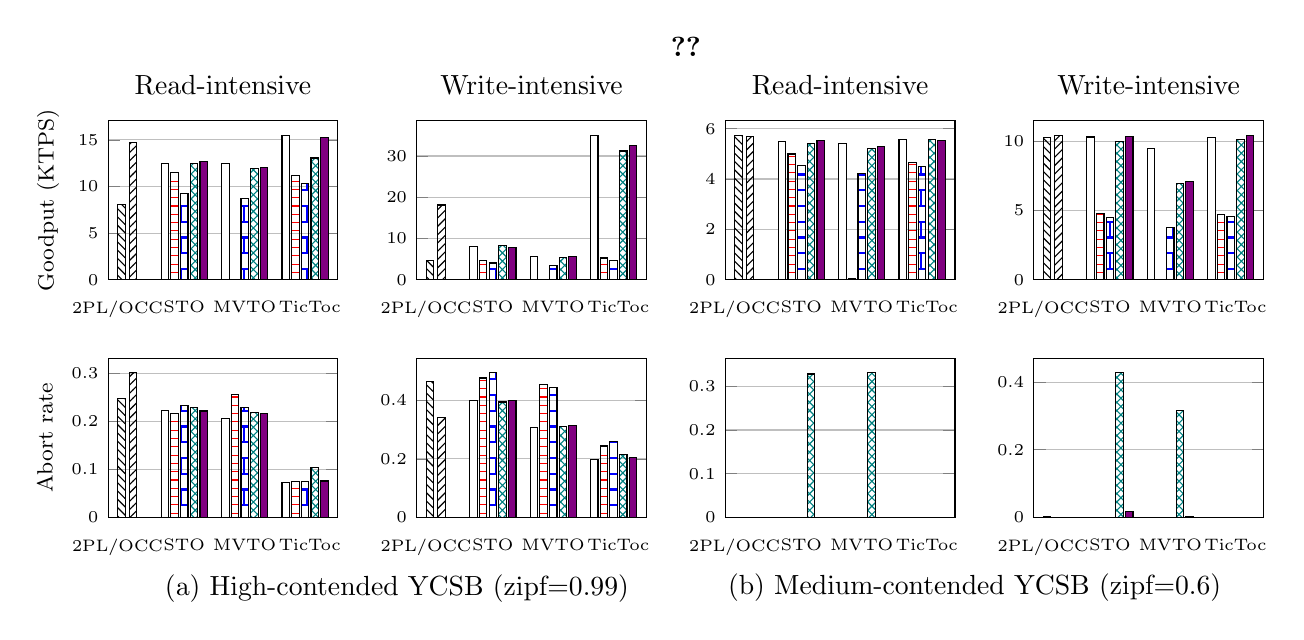
\begin{tikzpicture}
            \begin{groupplot}[group style={group size=4 by 2,
                            /pgf/bar width=2.7pt},
                    height = 3.6cm,
                    width = 4.5cm,
                    ybar= 2*\pgflinewidth,
                    xtick={-1, 0.425, 1.7125, 3.1},
                    xticklabels={2PL/OCC, STO, MVTO, TicToc},
                    ymajorgrids=true,
                    enlarge x limits = 0.2,
                    legend columns=-1,
                    legend entries={{\ssmall Memory (Idealized)}, {\ssmall Disk}, {\ssmall Disk-Cache}, {\ssmall \fsketchname},  {\ssmall \psketchname}},
                    area legend,
                    legend to name=grouplegend,
                ]

                % graph [1,1] high
                \nextgroupplot[title={Read-intensive},YCSBThroughputBarChartPlot, ylabel={Goodput (KTPS)}]
                \addplot[2PL-BarStyle, forget plot] coordinates {(-0.5, 8.04716)};
                \addplot[KR-OCC-BarStyle, forget plot] coordinates {(-0.26, 14.695467)};
                \addplot[Memory-BarStyle] coordinates {(0.425, 12.507633) (1.7125, 12.443733) (3, 15.512933)};
                \addplot[Disk-BarStyle] coordinates {(0.425, 11.482667) (1.7125, 0.032009) (3, 11.2091)};
                \addplot[Disk-Cache-BarStyle] coordinates {(0.425, 9.275193) (1.7125, 8.73535) (3, 10.287267)};
                \addplot[Counter-Lazy-BarStyle] coordinates {(0.425, 12.488167) (1.7125, 11.936367) (3, 13.065367)};
                \addplot[FPSketch-BarStyle] coordinates {(0.425, 12.669733) (1.7125, 11.999567) (3, 15.265833)};
                \coordinate (top) at (rel axis cs:0,1);% coordinate at top of the first plot

                % graph [1,3] high
                \nextgroupplot[title={Write-intensive}, YCSBThroughputBarChartPlot]
                \addplot[2PL-BarStyle, forget plot] coordinates {(-0.5, 4.608637)};
                \addplot[KR-OCC-BarStyle, forget plot] coordinates {(-0.26, 18.0974)};
                \addplot[Memory-BarStyle] coordinates {(0.425, 7.979627) (1.7125, 5.519357) (3, 35.047833)};
                \addplot[Disk-BarStyle] coordinates {(0.425, 4.551933) (1.7125, 0.022174) (3, 5.246687)};
                \addplot[Disk-Cache-BarStyle] coordinates {(0.425, 4.043277) (1.7125, 3.439533) (3, 4.70213)};
                \addplot[Counter-Lazy-BarStyle] coordinates {(0.425, 8.250597) (1.7125, 5.342587) (3, 31.205367)};
                \addplot[FPSketch-BarStyle] coordinates {(0.425, 7.749817) (1.7125, 5.59362) (3, 32.499733)};

                % graph [1,1] medium
                \nextgroupplot[title={Read-intensive},YCSBThroughputBarChartPlot]
                \addplot[2PL-BarStyle, forget plot] coordinates {(-0.5, 5.74492)};
                \addplot[KR-OCC-BarStyle, forget plot] coordinates {(-0.26, 5.701743)};
                \addplot[Memory-BarStyle] coordinates {(0.425, 5.495853) (1.7125, 5.41075) (3, 5.564913)};
                \addplot[Disk-BarStyle] coordinates {(0.425, 4.99792) (1.7125, 0.02941) (3, 4.655443)};
                \addplot[Disk-Cache-BarStyle] coordinates {(0.425, 4.54806) (1.7125, 4.207397) (3, 4.484957)};
                \addplot[Counter-Lazy-BarStyle] coordinates {(0.425, 5.40575) (1.7125, 5.208967) (3, 5.57541)};
                \addplot[FPSketch-BarStyle] coordinates {(0.425, 5.540247) (1.7125, 5.27708) (3, 5.5448)};


                % graph [1,3] medium
                \nextgroupplot[title={Write-intensive},YCSBThroughputBarChartPlot]
                \addplot[2PL-BarStyle, forget plot] coordinates {(-0.5, 10.272067)};
                \addplot[KR-OCC-BarStyle, forget plot] coordinates {(-0.26, 10.4202)};
                \addplot[Memory-BarStyle] coordinates {(0.425, 10.319067) (1.7125, 9.46724) (3, 10.3047)};
                \addplot[Disk-BarStyle] coordinates {(0.425, 4.80508) (1.7125, 0.029812) (3, 4.726683)};
                \addplot[Disk-Cache-BarStyle] coordinates {(0.425, 4.47477) (1.7125, 3.780167) (3, 4.576263)};
                \addplot[Counter-Lazy-BarStyle] coordinates {(0.425, 10.01148) (1.7125, 6.948757) (3, 10.13065)};
                \addplot[FPSketch-BarStyle] coordinates {(0.425, 10.33551) (1.7125, 7.09663) (3, 10.452133)};
                \coordinate (bot) at (rel axis cs:1,0);% coordinate at bottom of the last plot

                % graph [1,2] read intensive
                \nextgroupplot[AbortRateBarChartPlot, ylabel={Abort rate}]
                \addplot[2PL-BarStyle, forget plot] coordinates {(-0.5, 0.247383)};
                \addplot[KR-OCC-BarStyle, forget plot] coordinates {(-0.26, 0.301227)};
                \addplot[Memory-BarStyle] coordinates {(0.425, 0.222445) (1.7125, 0.206034) (3, 0.07278)};
                \addplot[Disk-BarStyle] coordinates {(0.425, 0.21628) (1.7125, 0.25627) (3, 0.074478)};
                \addplot[Disk-Cache-BarStyle] coordinates {(0.425, 0.23351) (1.7125, 0.228067) (3, 0.073814)};
                \addplot[Counter-Lazy-BarStyle] coordinates {(0.425, 0.228598) (1.7125, 0.218929) (3, 0.103984)};
                \addplot[FPSketch-BarStyle] coordinates {(0.425, 0.221732) (1.7125, 0.216595) (3, 0.075632)};

                % graph [1,4] write intensive
                \nextgroupplot[AbortRateBarChartPlot]
                \addplot[2PL-BarStyle, forget plot] coordinates {(-0.5, 0.465557)};
                \addplot[KR-OCC-BarStyle, forget plot] coordinates {(-0.26, 0.34286)};
                \addplot[Memory-BarStyle] coordinates {(0.425, 0.400389) (1.7125, 0.306523) (3, 0.197603)};
                \addplot[Disk-BarStyle] coordinates {(0.425, 0.476595) (1.7125, 0.454508) (3, 0.243955)};
                \addplot[Disk-Cache-BarStyle] coordinates {(0.425, 0.494111) (1.7125, 0.444139) (3, 0.258452)};
                \addplot[Counter-Lazy-BarStyle] coordinates {(0.425, 0.394383) (1.7125, 0.309213) (3, 0.21479)};
                \addplot[FPSketch-BarStyle] coordinates {(0.425, 0.399936) (1.7125, 0.315027) (3, 0.203892)};

                % graph [1,2]
                \nextgroupplot[AbortRateBarChartPlot]
                \addplot[2PL-BarStyle, forget plot] coordinates {(-0.5, 0.000222)};
                \addplot[KR-OCC-BarStyle, forget plot] coordinates {(-0.26, 0.00011)};
                \addplot[Memory-BarStyle] coordinates {(0.425, 0.000047) (1.7125, 0.000047) (3, 0.000017)};
                \addplot[Disk-BarStyle] coordinates {(0.425, 0.000039) (1.7125, 0.000046) (3, 0.000024)};
                \addplot[Disk-Cache-BarStyle] coordinates {(0.425, 0.000045) (1.7125, 0.000044) (3, 0.000016)};
                \addplot[Counter-Lazy-BarStyle] coordinates {(0.425, 0.328226) (1.7125, 0.330902) (3, 0.000046)};
                \addplot[FPSketch-BarStyle] coordinates {(0.425, 0.000279) (1.7125, 0.000117) (3, 0.000039)};

                % graph [1,4]
                \nextgroupplot[AbortRateBarChartPlot]
                \addplot[2PL-BarStyle, forget plot] coordinates {(-0.5, 0.001511)};
                \addplot[KR-OCC-BarStyle, forget plot] coordinates {(-0.26, 0.000493)};
                \addplot[Memory-BarStyle] coordinates {(0.425, 0.000238) (1.7125, 0.000219) (3, 0.000093)};
                \addplot[Disk-BarStyle] coordinates {(0.425, 0.000276) (1.7125, 0.000137) (3, 0.000174)};
                \addplot[Disk-Cache-BarStyle] coordinates {(0.425, 0.000238) (1.7125, 0.000242) (3, 0.00018)};
                \addplot[Counter-Lazy-BarStyle] coordinates {(0.425, 0.427524) (1.7125, 0.3174) (3, 0.00022)};
                \addplot[FPSketch-BarStyle] coordinates {(0.425, 0.016898) (1.7125, 0.003473) (3, 0.000212)};

            \end{groupplot}
            \coordinate (c) at ($(top)!.5!(bot)$);
            \coordinate (cc1) at ($(top)!.25!(bot)$);
            \coordinate (cc2) at ($(top)!.75!(bot)$);

            \node[above] at (c |- current bounding box.north) {\ref{grouplegend}};
            \node[below] at (cc1 |- current bounding box.south) {(a) High-contended YCSB (zipf=0.99)};
            \node[above] at (cc2 |- current bounding box.south) {(b) Medium-contended YCSB (zipf=0.6)};
        \end{tikzpicture}
    } \caption[YCSB small-transaction workloads results on HDD]{YCSB
    small-transaction workloads results with 60 processing threads on HDD. In
    write-intensive workloads, each transaction performs 8 reads and 8 writes.
    In read-intensive workloads, each transaction performs 15 reads and 1 write.
    Note that, in the medium-contended workload, several variants have abort
    rates very close to 0.}
    \label{fig:ycsb:slow_hdd}
\end{figure}


\Cref{fig:ycsb:slow_hdd} shows the results of running YCSB small-transaction
workloads with 60 processing threads on an HDD. In the high-contention,
read-intensive workload, KR-OCC reaches about 14 KTPS. Because disk I/O is a
major bottleneck with slow storage, KR-OCC performs better than other
timestamp-based concurrency control (CC) methods except for TicToc.
TicToc-\psketchname has the highest goodput in this workload, running 1.04 times
faster than KR-OCC. In addition, \psketchname increases TicToc's goodput by 36\%
compared to TicToc-Disk.

Similar to the results in \Cref{fig:ycsb:slow_ssd}, when the workload is
high-contention and write-intensive, \sketchname keeps TicToc's high
performance. TicToc-\psketchname achieves 1.8 times the speed of KR-OCC and
increases goodput by 519\% compared to TicToc-Disk.

For workloads with medium contention, all methods are mainly limited by I/O. The
Disk versions have extra I/O overhead to get timestamps. \sketchname removes
this overhead, increasing goodput by up to 19\% and 121\% for the read-intensive
and the write-intensive workloads, respectively.



\subsubsection{YCSB Mixed-Transaction Workloads}


\begin{figure}[!t]
    \centering
    \resizebox{\textwidth}{!}{%
        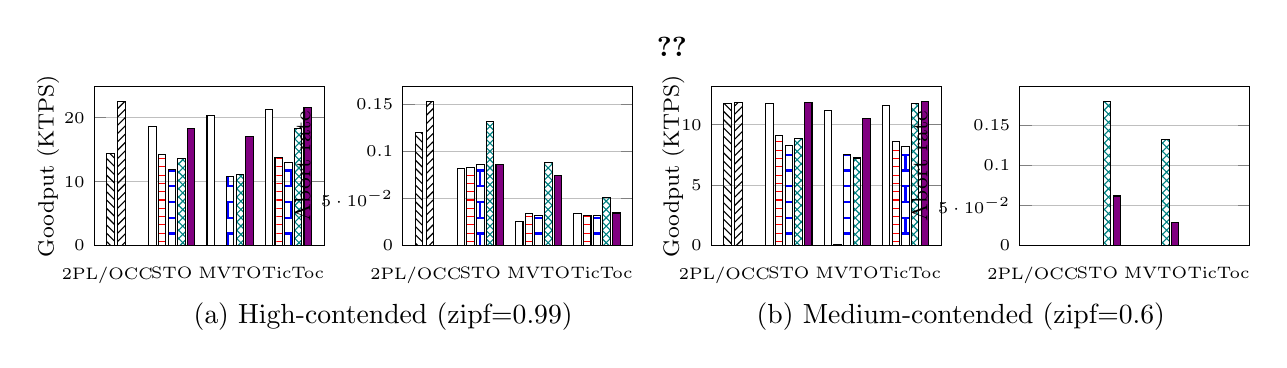
\begin{tikzpicture}
            \begin{groupplot}[group style={group size=4 by 1,
                            /pgf/bar width=2.7pt},
                    height = 3.6cm,
                    width = 4.5cm,
                    ybar= 2*\pgflinewidth,
                    xtick={-1, 0.425, 1.7125, 3.1},
                    xticklabels={2PL/OCC, STO, MVTO, TicToc},
                    ymajorgrids=true,
                    enlarge x limits = 0.225,
                    legend columns=-1,
                    legend entries={{\ssmall Memory (Idealized)}, {\ssmall Disk}, {\ssmall Disk-Cache}, {\ssmall \fsketchname},  {\ssmall \psketchname}},
                    area legend,
                    legend to name=grouplegend,
                ]

                % graph [1,1] high
                \nextgroupplot[YCSBThroughputBarChartPlot, ylabel={Goodput (KTPS)}, ylabel style={yshift=-5pt}]
                \addplot[2PL-BarStyle, forget plot] coordinates {(-0.5, 14.398367)};
                \addplot[KR-OCC-BarStyle, forget plot] coordinates {(-0.26, 22.5943)};
                \addplot[Memory-BarStyle] coordinates {(0.425, 18.620767) (1.7125, 20.2924) (3, 21.2467)};
                \addplot[Disk-BarStyle] coordinates {(0.425, 14.2852) (1.7125, 0.057283) (3, 13.813567)};
                \addplot[Disk-Cache-BarStyle] coordinates {(0.425, 11.8618) (1.7125, 10.774433) (3, 12.974133)};
                \addplot[Counter-Lazy-BarStyle] coordinates {(0.425, 13.572667) (1.7125, 11.1527) (3, 18.250733)};
                \addplot[FPSketch-BarStyle] coordinates {(0.425, 18.253) (1.7125, 17.012867) (3, 21.638033)};
                \coordinate (top) at (rel axis cs:0,1);% coordinate at top of the first plot

                % graph [2,1] abort rate
                \nextgroupplot[AbortRateBarChartPlot, ylabel={Abort rate}, ylabel style={yshift=-3pt}]
                \addplot[2PL-BarStyle, forget plot] coordinates {(-0.5, 0.120156)};
                \addplot[KR-OCC-BarStyle, forget plot] coordinates {(-0.26, 0.153397)};
                \addplot[Memory-BarStyle] coordinates {(0.425, 0.081903) (1.7125, 0.025545) (3, 0.034029)};
                \addplot[Disk-BarStyle] coordinates {(0.425, 0.083356) (1.7125, 0.034113) (3, 0.032248)};
                \addplot[Disk-Cache-BarStyle] coordinates {(0.425, 0.085848) (1.7125, 0.031777) (3, 0.031905)};
                \addplot[Counter-Lazy-BarStyle] coordinates {(0.425, 0.131356) (1.7125, 0.088476) (3, 0.05094)};
                \addplot[FPSketch-BarStyle] coordinates {(0.425, 0.086357) (1.7125, 0.07476) (3, 0.034597)};

                % graph [3,1] medium
                \nextgroupplot[YCSBThroughputBarChartPlot, ylabel={Goodput (KTPS)}, ylabel style={yshift=-8pt}]
                \addplot[2PL-BarStyle, forget plot] coordinates {(-0.5, 11.759533)};
                \addplot[KR-OCC-BarStyle, forget plot] coordinates {(-0.26, 11.808467)};
                \addplot[Memory-BarStyle] coordinates {(0.425, 11.777167) (1.7125, 11.1943) (3, 11.590367)};
                \addplot[Disk-BarStyle] coordinates {(0.425, 9.137557) (1.7125, 0.053173) (3, 8.6221)};
                \addplot[Disk-Cache-BarStyle] coordinates {(0.425, 8.24723) (1.7125, 7.554443) (3, 8.227663)};
                \addplot[Counter-Lazy-BarStyle] coordinates {(0.425, 8.86626) (1.7125, 7.247293) (3, 11.721167)};
                \addplot[FPSketch-BarStyle] coordinates {(0.425, 11.8456) (1.7125, 10.549667) (3, 11.9516)};

                % graph [4,1] medium abort rate
                \nextgroupplot[AbortRateBarChartPlot, ylabel={Abort rate}, ylabel style={yshift=-3pt}]
                \addplot[2PL-BarStyle, forget plot] coordinates {(-0.5, 0.000225)};
                \addplot[KR-OCC-BarStyle, forget plot] coordinates {(-0.26, 0.000255)};
                \addplot[Memory-BarStyle] coordinates {(0.425, 0.000116) (1.7125, 0.000018) (3, 0.000039)};
                \addplot[Disk-BarStyle] coordinates {(0.425, 0.000103) (1.7125, 0.000052) (3, 0.000041)};
                \addplot[Disk-Cache-BarStyle] coordinates {(0.425, 0.000092) (1.7125, 0.000077) (3, 0.000034)};
                \addplot[Counter-Lazy-BarStyle] coordinates {(0.425, 0.180175) (1.7125, 0.132656) (3, 0.000122)};
                \addplot[FPSketch-BarStyle] coordinates {(0.425, 0.061843) (1.7125, 0.029213) (3, 0.00009)};
                \coordinate (bot) at (rel axis cs:1,0);% coordinate at bottom of the last plot

            \end{groupplot}
            \coordinate (c) at ($(top)!.5!(bot)$);
            \coordinate (cc1) at ($(top)!.25!(bot)$);
            \coordinate (cc2) at ($(top)!.75!(bot)$);

            \node[above] at (c |- current bounding box.north) {\ref{grouplegend}};
            \node[below] at (cc1 |- current bounding box.south) {(a) High-contended (zipf=0.99)};
            \node[above] at (cc2 |- current bounding box.south) {(b) Medium-contended (zipf=0.6)};
        \end{tikzpicture}
    } \caption[YCSB mixed-transaction workloads results on HDD]{YCSB
    mixed-transaction workloads results with 60 processing threads on HDD. 80\%
    of transactions perform 2 reads and 2 writes, and 20\% of transactions
    perform 28 reads. Note that, in the medium-contended workload, several
    variants have abort rates very close to 0.}
    \label{fig:ycsb:mixed:hdd}
\end{figure}

\Cref{fig:ycsb:mixed:hdd} shows the results of running YCSB mixed-transaction
workloads with 60 processing threads on an HDD. The results are similar to the
read-intensive workload results on HDD in \Cref{fig:ycsb:slow_hdd} because 20\%
of transactions perform 28 reads. TicToc-\psketchname is 0.96$\times$ slower
than KR-OCC but it increases goodput by 56.6\% compared to TicToc-Disk.



\subsubsection{YCSB Long-Transaction Workload}



\begin{figure}[!t]
    \centering
    \resizebox{.75\textwidth}{!}{%
        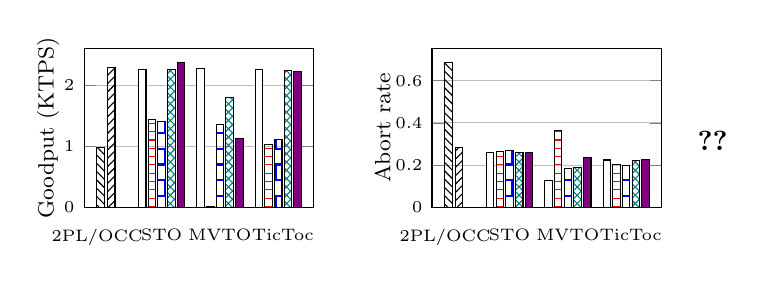
\begin{tikzpicture}
            \begin{groupplot}[group style={
                            group size=2 by 1,
                            horizontal sep=1.5cm,
                            /pgf/bar width=2.7pt
                        },
                    height = 3.6cm,
                    width = 4.5cm,
                    ybar= 2*\pgflinewidth,
                    xtick={-1, 0.425, 1.7125, 3.1},
                    xticklabels={2PL/OCC, STO, MVTO, TicToc},
                    ymajorgrids=true,
                    enlarge x limits = 0.225,
                    legend columns=1,
                    legend entries={{\ssmall Memory (Idealized)}, {\ssmall Disk}, {\ssmall Disk-Cache}, {\ssmall \fsketchname},  {\ssmall \psketchname}},
                    area legend,
                    legend to name=grouplegend,
                ]

                % graph [1,1] high
                \nextgroupplot[YCSBThroughputBarChartPlot, ylabel={Goodput (KTPS)}, ylabel style={yshift=-5pt}]
                \addplot[2PL-BarStyle, forget plot] coordinates {(-0.5, 0.978672)};
                \addplot[KR-OCC-BarStyle, forget plot] coordinates {(-0.26, 2.292817)};
                \addplot[Memory-BarStyle] coordinates {(0.425, 2.254873) (1.7125, 2.272397) (3, 2.263723)};
                \addplot[Disk-BarStyle] coordinates {(0.425, 1.441723) (1.7125, 0.006307) (3, 1.035913)};
                \addplot[Disk-Cache-BarStyle] coordinates {(0.425, 1.399493) (1.7125, 1.361513) (3, 1.10648)};
                \addplot[Counter-Lazy-BarStyle] coordinates {(0.425, 2.25934) (1.7125, 1.798883) (3, 2.244893)};
                \addplot[FPSketch-BarStyle] coordinates {(0.425, 2.364233) (1.7125, 1.121917) (3, 2.22647)};
                \coordinate (top) at (rel axis cs:0,1);% coordinate at top of the first plot

                % graph [1,2] abort rate
                \nextgroupplot[AbortRateBarChartPlot, ylabel={Abort rate}, ylabel style={yshift=-5pt}]
                \addplot[2PL-BarStyle, forget plot] coordinates {(-0.5, 0.684035)};
                \addplot[KR-OCC-BarStyle, forget plot] coordinates {(-0.26, 0.282721)}; % double check
                \addplot[Memory-BarStyle] coordinates {(0.425, 0.259254) (1.7125, 0.128753) (3, 0.224552)};
                \addplot[Disk-BarStyle] coordinates {(0.425, 0.264165) (1.7125, 0.365076) (3, 0.204642)}; % double check mvcc
                \addplot[Disk-Cache-BarStyle] coordinates {(0.425, 0.270411) (1.7125, 0.182728) (3, 0.199765)}; % rerun
                \addplot[Counter-Lazy-BarStyle] coordinates {(0.425, 0.258943) (1.7125, 0.189777) (3, 0.222702)};
                \addplot[FPSketch-BarStyle] coordinates {(0.425, 0.259826) (1.7125, 0.234995) (3, 0.227486)};
                \coordinate (bot) at (rel axis cs:1,0);% coordinate at bottom of the last plot

            \end{groupplot}
            \coordinate (c) at ($(top)!.5!(bot)$);

            \node[right=4cm] at (c |- current bounding box.east) {\ref{grouplegend}};
        \end{tikzpicture}
    } \caption[YCSB long-transaction workloads results on HDD]{YCSB
    long-transaction workloads results with 60 processing threads on HDD. 5\% of
    transactions perform 1000 reads and the rest of transactions perform 8
    writes and 8 reads. The distribution is Zipfian with 0.9.}
    \label{fig:ycsb:long:hdd}
\end{figure}

As the slow disk is a major bottleneck in read-intensive workloads, all methods
except 2PL show similar goodput, while 2PL causes higher abort rates. \sketchname
variants show their effectiveness in removing the need to access timestamps on
disk, resulting in higher goodput. However, MVTO with \sketchname incurs extra
write operations as described in \Cref{sec:fpsketch:mvto}, resulting in lower
goodput.


\subsubsection{TPC-C Workloads}

\begin{figure*}[!t]
    \centering
    \resizebox{\textwidth}{!}{%
        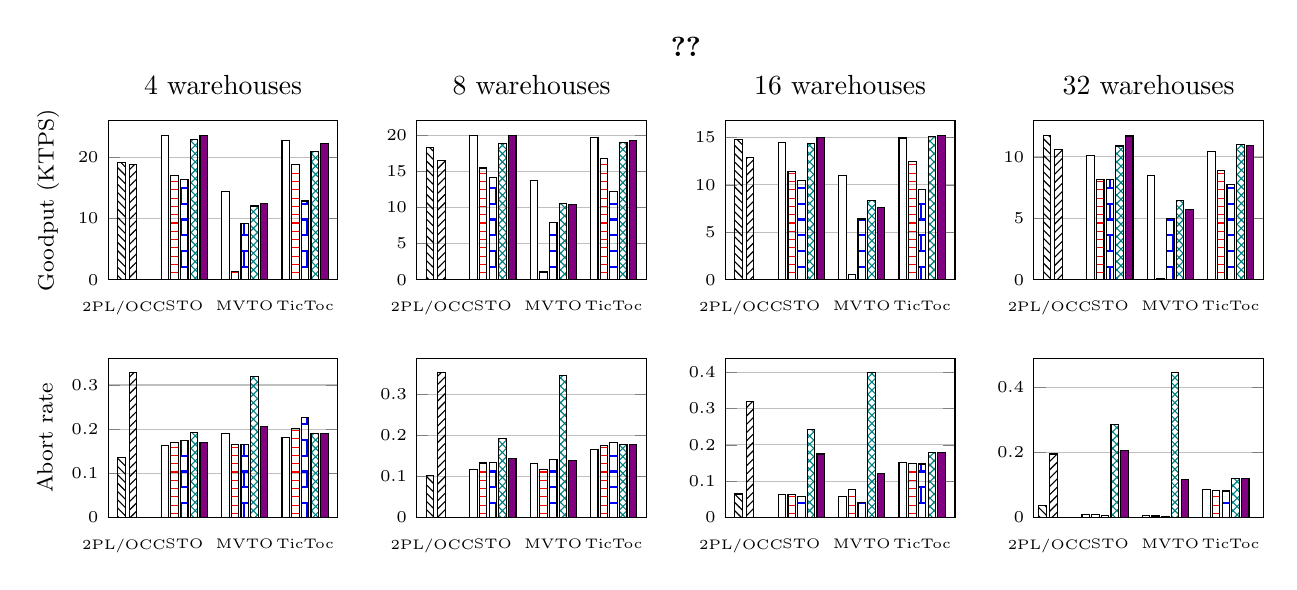
\begin{tikzpicture}
            \begin{groupplot}[group style={group size=4 by 2,
                            /pgf/bar width=2.7pt},
                    height = 3.6cm,
                    width = 4.5cm,
                    ybar= 2*\pgflinewidth,
                    xtick={-0.8625, 0.425, 1.7125, 3},
                    xticklabels={2PL/OCC, STO, MVTO, TicToc},
                    xticklabel style={font=\tiny},
                    ymajorgrids=true,
                    enlarge x limits = 0.2,
                    legend columns=-1,
                    legend entries={{\ssmall Memory (Idealized)}, {\ssmall Disk}, {\ssmall Disk-Cache}, {\ssmall \fsketchname},  {\ssmall \psketchname}},
                    area legend,
                    legend to name=grouplegend,
                ]

                % graph [1,1]
                \nextgroupplot[title={4 warehouses},YCSBThroughputBarChartPlot, ylabel={Goodput (KTPS)}]
                \addplot[2PL-BarStyle, forget plot] coordinates {(-0.5, 19.115367)};
                \addplot[KR-OCC-BarStyle, forget plot] coordinates {(-0.26, 18.856033)};
                \addplot[Memory-BarStyle] coordinates {(0.425, 23.608167) (1.7125, 14.4289) (3, 22.799833)};
                \addplot[Disk-BarStyle] coordinates {(0.425, 16.973967) (1.7125, 1.393113) (3, 18.8406)};
                \addplot[Disk-Cache-BarStyle] coordinates {(0.425, 16.312733) (1.7125, 9.138087) (3, 12.860733)};
                \addplot[Counter-Lazy-BarStyle] coordinates {(0.425, 22.9111) (1.7125, 12.039267) (3, 20.9325)};
                \addplot[FPSketch-BarStyle] coordinates {(0.425, 23.628533) (1.7125, 12.440333) (3, 22.200533)};
                \coordinate (top) at (rel axis cs:0,1);% coordinate at top of the first plot

                % graph [1,2]
                \nextgroupplot[title={8 warehouses}, YCSBThroughputBarChartPlot]
                \addplot[2PL-BarStyle, forget plot] coordinates {(-0.5, 18.381033)};
                \addplot[KR-OCC-BarStyle, forget plot] coordinates {(-0.26, 16.4903)};
                \addplot[Memory-BarStyle] coordinates {(0.425, 19.961433) (1.7125, 13.819533) (3, 19.699833)};
                \addplot[Disk-BarStyle] coordinates {(0.425, 15.508133) (1.7125, 1.069157) (3, 16.799167)};
                \addplot[Disk-Cache-BarStyle] coordinates {(0.425, 14.151633) (1.7125, 7.96076) (3, 12.205833)};
                \addplot[Counter-Lazy-BarStyle] coordinates {(0.425, 18.863267) (1.7125, 10.526333) (3, 19.065667)};
                \addplot[FPSketch-BarStyle] coordinates {(0.425, 20.064667) (1.7125, 10.490667) (3, 19.3602)};

                % graph [1,3]
                \nextgroupplot[title={16 warehouses},YCSBThroughputBarChartPlot]
                \addplot[2PL-BarStyle, forget plot] coordinates {(-0.5, 14.7968)};
                \addplot[KR-OCC-BarStyle, forget plot] coordinates {(-0.26, 12.914467)};
                \addplot[Memory-BarStyle] coordinates {(0.425, 14.465267) (1.7125, 10.981267) (3, 14.941067)};
                \addplot[Disk-BarStyle] coordinates {(0.425, 11.4572) (1.7125, 0.588741) (3, 12.457133)};
                \addplot[Disk-Cache-BarStyle] coordinates {(0.425, 10.463967) (1.7125, 6.40315) (3, 9.55108)};
                \addplot[Counter-Lazy-BarStyle] coordinates {(0.425, 14.398667) (1.7125, 8.379683) (3, 15.104167)};
                \addplot[FPSketch-BarStyle] coordinates {(0.425, 15.039833) (1.7125, 7.637783) (3, 15.2448)};


                % graph [1,4] 32wh
                \nextgroupplot[title={32 warehouses},YCSBThroughputBarChartPlot]
                \addplot[2PL-BarStyle, forget plot] coordinates {(-0.5, 11.7632)};
                \addplot[KR-OCC-BarStyle, forget plot] coordinates {(-0.26, 10.5966)};
                \addplot[Memory-BarStyle] coordinates {(0.425, 10.126013) (1.7125, 8.492203) (3, 10.425733)};
                \addplot[Disk-BarStyle] coordinates {(0.425, 8.154903) (1.7125, 0.066267) (3, 8.868137)};
                \addplot[Disk-Cache-BarStyle] coordinates {(0.425, 8.18903) (1.7125, 5.0047) (3, 7.765507)};
                \addplot[Counter-Lazy-BarStyle] coordinates {(0.425, 10.880967) (1.7125, 6.456127) (3, 10.9942)};
                \addplot[FPSketch-BarStyle] coordinates {(0.425, 11.699533) (1.7125, 5.712097) (3, 10.9556)};

                \coordinate (bot) at (rel axis cs:1,0);% coordinate at bottom of the last plot

                % graph [2,1] 4 wh
                \nextgroupplot[AbortRateBarChartPlot, ylabel={Abort rate}]
                \addplot[2PL-BarStyle, forget plot] coordinates {(-0.5, 0.135487)};
                \addplot[KR-OCC-BarStyle, forget plot] coordinates {(-0.26, 0.327479)};
                \addplot[Memory-BarStyle] coordinates {(0.425, 0.16263) (1.7125, 0.190511) (3, 0.181326)};
                \addplot[Disk-BarStyle] coordinates {(0.425, 0.168929) (1.7125, 0.164452) (3, 0.201198)};
                \addplot[Disk-Cache-BarStyle] coordinates {(0.425, 0.173134) (1.7125, 0.164581) (3, 0.226057)};
                \addplot[Counter-Lazy-BarStyle] coordinates {(0.425, 0.193154) (1.7125, 0.318299) (3, 0.188983)};
                \addplot[FPSketch-BarStyle] coordinates {(0.425, 0.170551) (1.7125, 0.205813) (3, 0.189242)};

                % graph [2,2] 8 wh
                \nextgroupplot[AbortRateBarChartPlot]
                \addplot[2PL-BarStyle, forget plot] coordinates {(-0.5, 0.102231)};
                \addplot[KR-OCC-BarStyle, forget plot] coordinates {(-0.26, 0.352503)};
                \addplot[Memory-BarStyle] coordinates {(0.425, 0.116895) (1.7125, 0.130499) (3, 0.165533)};
                \addplot[Disk-BarStyle] coordinates {(0.425, 0.13252) (1.7125, 0.11766) (3, 0.176234)};
                \addplot[Disk-Cache-BarStyle] coordinates {(0.425, 0.134825) (1.7125, 0.140453) (3, 0.183218)};
                \addplot[Counter-Lazy-BarStyle] coordinates {(0.425, 0.192119) (1.7125, 0.345666) (3, 0.177427)};
                \addplot[FPSketch-BarStyle] coordinates {(0.425, 0.144327) (1.7125, 0.138727) (3, 0.178054)};

                % graph [2,3] 16 wh
                \nextgroupplot[AbortRateBarChartPlot]
                \addplot[2PL-BarStyle, forget plot] coordinates {(-0.5, 0.064185)};
                \addplot[KR-OCC-BarStyle, forget plot] coordinates {(-0.26, 0.318935)};
                \addplot[Memory-BarStyle] coordinates {(0.425, 0.063774) (1.7125, 0.056843) (3, 0.15089)};
                \addplot[Disk-BarStyle] coordinates {(0.425, 0.062464) (1.7125, 0.075799) (3, 0.14947)};
                \addplot[Disk-Cache-BarStyle] coordinates {(0.425, 0.056327) (1.7125, 0.039754) (3, 0.147102)};
                \addplot[Counter-Lazy-BarStyle] coordinates {(0.425, 0.243272) (1.7125, 0.398401) (3, 0.178241)};
                \addplot[FPSketch-BarStyle] coordinates {(0.425, 0.17467) (1.7125, 0.121197) (3, 0.178254)};

                % graph [2,4] 32 wh
                \nextgroupplot[AbortRateBarChartPlot]
                \addplot[2PL-BarStyle, forget plot] coordinates {(-0.5, 0.036227)};
                \addplot[KR-OCC-BarStyle, forget plot] coordinates {(-0.26, 0.195207)};
                \addplot[Memory-BarStyle] coordinates {(0.425, 0.008601) (1.7125, 0.006069) (3, 0.086278)};
                \addplot[Disk-BarStyle] coordinates {(0.425, 0.007884) (1.7125, 0.004012) (3, 0.082685)};
                \addplot[Disk-Cache-BarStyle] coordinates {(0.425, 0.004574) (1.7125, 0.002209) (3, 0.081135)};
                \addplot[Counter-Lazy-BarStyle] coordinates {(0.425, 0.28479) (1.7125, 0.445157) (3, 0.12057)};
                \addplot[FPSketch-BarStyle] coordinates {(0.425, 0.20554) (1.7125, 0.116253) (3, 0.11906)};

                \addplot[Disk-Cache-BarStyle] coordinates {(0.425, 0) (1.7125, 0) (3, 0)};

            \end{groupplot}
            \coordinate (c) at ($(top)!.5!(bot)$);

            \node[above] at (c |- current bounding box.north) {\ref{grouplegend}};
        \end{tikzpicture}
    } \caption[TPC-C results on HDD]{TPC-C results with 60 processing threads
    on HDD (More warehouses means less contention).}
    \label{fig:tpcc:hdd}
\end{figure*}

Figure~\ref{fig:tpcc:hdd} presents the goodput results for the TPC-C workloads
described in \Cref{sec:eval-setup}, but now running on an HDD. As seen with the
YCSB experiments on HDD, \sketchname performs very well in high-contention
situations with a small number of warehouses. When contention is lower, however,
the performance of all concurrency control methods becomes similar because the
speed of the slow hard drive limits throughput. With 4 warehouses,
STO-\psketchname and TicToc-\psketchname achieve up to 1.25$\times$ and
1.18$\times$ better goodput than 2PL/KR-OCC, respectively.



\section{Fast Storage}\label{sec:fast-storage}

Having demonstrated \sketchname's effectiveness on slow storage, we now evaluate
its performance on fast storage media, such as CXL-based flash with DRAM-like 
latency. This evaluation reveals a fundamental shift in performance 
characteristics: as storage becomes faster, the system transitions from being 
I/O-bound to CPU-bound, making the overhead of the \sketchname data structure 
itself more visible relative to storage access costs. These results provide 
insights into how \sketchname variants scale as storage technologies continue to 
evolve toward lower latencies.

\subsection{CXL Emulation Methodology}

To evaluate \sketchname's effectiveness on next-generation storage technologies,
we emulate CXL-based flash storage using block ramdisk. This subsection details
our emulation methodology, the assumptions we make, and how our results relate to
real CXL hardware.

\subsubsection{Emulation Setup}

We use block ramdisk on the same CloudLab machine described in \Cref{sec:eval-setup}
to emulate CXL-based flash with DRAM-like latency. Block ramdisk provides storage
access through the standard block device interface while storing data in RAM,
effectively creating a software-based storage layer that mimics the low latency
characteristics of memory-like storage technologies. This approach allows us to
evaluate \sketchname's behavior when storage access times are dramatically reduced
without requiring specialized CXL hardware that may not be readily available in
experimental environments.

The emulated storage provides latencies approximately 100$\times$ faster than SATA
SSD and 10$\times$ faster than NVMe SSD, closely approximating the characteristics
of next-generation CXL-based storage. Specifically, while NVMe SSDs achieve
latencies in the 20--100 microsecond range, CXL-based storage targets latencies in
the single-digit microsecond range (1--10 microseconds). Our block ramdisk
emulation achieves latencies on the order of hundreds of nanoseconds, providing a
reasonable approximation of CXL performance characteristics for the purpose of
understanding how \sketchname scales as storage becomes faster.

\subsubsection{Assumptions and Limitations}

Our emulation makes several important assumptions that should be considered when
interpreting results:

\begin{itemize}
    \item \textbf{Interface semantics}: Block ramdisk uses the standard block
    device interface, whereas real CXL storage may support byte-addressable access
    through the CXL.mem protocol. This difference may affect the relative
    performance of different access patterns, though the fundamental latency
    characteristics we seek to emulate are preserved.
    
    \item \textbf{Bandwidth characteristics}: Real CXL storage provides high
    bandwidth (up to 16 GB/s on PCIe 5.0 x4), whereas our emulation is limited by
    system RAM bandwidth. However, since our evaluation focuses on latency-bound
    operations (random I/O for timestamp access), bandwidth differences have minimal
    impact on our findings.
    
    \item \textbf{Remote memory effects}: Real CXL storage may exhibit NUMA-like
    behavior with remote memory access characteristics. Our emulation does not
    capture these effects, though \sketchname's effectiveness in avoiding remote
    access overhead remains valid.
    
    \item \textbf{CPU overhead}: Block ramdisk still incurs some software overhead
    from the block device stack, whereas real CXL storage with direct memory access
    may have different overhead characteristics. However, this overhead is minimal
    compared to actual storage latency and does not materially affect our
    conclusions.
\end{itemize}

\subsubsection{Experimental Configuration}

In these fast storage experiments, we evaluate only STO and TicToc protocols.
MVTO runs out of memory on the machine with 256GB of memory because its write
operations keep creating new versions of keys, making it impractical for
evaluation on fast storage where write rates are extremely high. We run 120
processing threads for all experiments, matching the configuration used in our
NVMe SSD evaluations. All other experimental parameters (workloads, database size,
cache configurations) remain consistent with the evaluations described in
\Cref{sec:eval-setup} to ensure fair comparison across storage types.

The following sections present results showing that \sketchname variants
significantly outperform 2PL and KR-OCC on fast storage, achieving dramatic
improvements in high-contention scenarios while maintaining effectiveness across
all workload types. However, the relative overhead of \sketchname operations
becomes more pronounced, revealing areas for future optimization.

\subsubsection{YCSB Small-Transaction Workloads}


\begin{figure}[!t]
    \centering
    \resizebox{\textwidth}{!}{%
        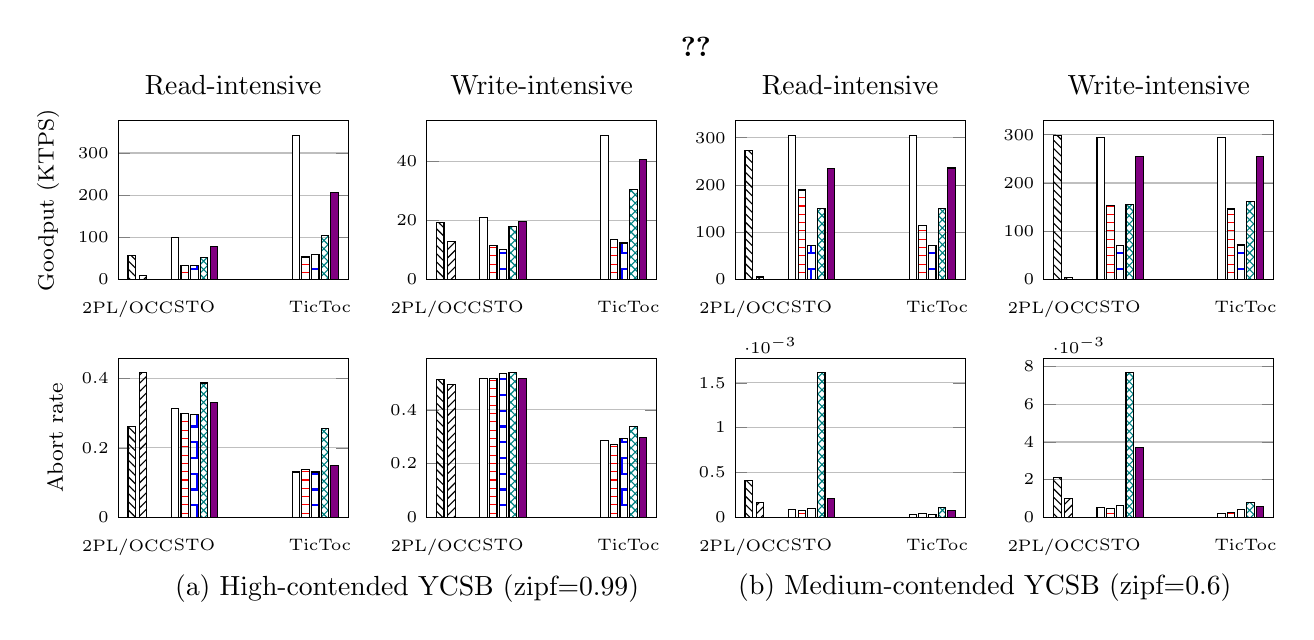
\begin{tikzpicture}
            \begin{groupplot}[group style={group size=4 by 2,
                            /pgf/bar width=2.7pt},
                    height = 3.6cm,
                    width = 4.5cm,
                    ybar= 2*\pgflinewidth,
                    xtick={-1, 0.425, 3.1},
                    xticklabels={2PL/OCC, STO, TicToc},
                    ymajorgrids=true,
                    enlarge x limits = 0.2,
                    legend columns=-1,
                    legend entries={{\ssmall Memory (Idealized)}, {\ssmall Disk}, {\ssmall Disk-Cache}, {\ssmall \fsketchname},  {\ssmall \psketchname}},
                    area legend,
                    legend to name=grouplegend,
                ]

                % graph [1,1] high
                \nextgroupplot[title={Read-intensive},YCSBThroughputBarChartPlot, ylabel={Goodput (KTPS)}]
                \addplot[2PL-BarStyle, forget plot] coordinates {(-0.5, 58.2401)};
                \addplot[KR-OCC-BarStyle, forget plot] coordinates {(-0.26, 9.641523)};
                \addplot[Memory-BarStyle] coordinates {(0.425, 100.589433) (3, 342.33)};
                \addplot[Disk-BarStyle] coordinates {(0.425, 32.581733) (3, 53.617733)};
                \addplot[Disk-Cache-BarStyle] coordinates {(0.425, 34.518667) (3, 60.1803)};
                \addplot[Counter-Lazy-BarStyle] coordinates {(0.425, 52.053633) (3, 105.591)};
                \addplot[FPSketch-BarStyle] coordinates {(0.425, 78.006133) (3, 206.962)};
                \coordinate (top) at (rel axis cs:0,1);% coordinate at top of the first plot

                % graph [1,3] high
                \nextgroupplot[title={Write-intensive}, YCSBThroughputBarChartPlot]
                \addplot[2PL-BarStyle, forget plot] coordinates {(-0.5, 19.146733)};
                \addplot[KR-OCC-BarStyle, forget plot] coordinates {(-0.26, 12.871567)};
                \addplot[Memory-BarStyle] coordinates {(0.425, 20.868633) (3, 48.751833)};
                \addplot[Disk-BarStyle] coordinates {(0.425, 11.414233) (3, 13.5591)};
                \addplot[Disk-Cache-BarStyle] coordinates {(0.425, 10.320467) (3, 12.3741)};
                \addplot[Counter-Lazy-BarStyle] coordinates {(0.425, 17.8436) (3, 30.488667)};
                \addplot[FPSketch-BarStyle] coordinates {(0.425, 19.657167) (3, 40.6375)};

                % graph [1,1] medium
                \nextgroupplot[title={Read-intensive},YCSBThroughputBarChartPlot]
                \addplot[2PL-BarStyle, forget plot] coordinates {(-0.5, 272.525667)};
                \addplot[KR-OCC-BarStyle, forget plot] coordinates {(-0.26, 5.632817)};
                \addplot[Memory-BarStyle] coordinates {(0.425, 304.898) (3, 305.503333)};
                \addplot[Disk-BarStyle] coordinates {(0.425, 189.604) (3, 113.674333)};
                \addplot[Disk-Cache-BarStyle] coordinates {(0.425, 71.498267) (3, 71.392467)};
                \addplot[Counter-Lazy-BarStyle] coordinates {(0.425, 149.862667) (3, 151.15)};
                \addplot[FPSketch-BarStyle] coordinates {(0.425, 235.684667) (3, 235.993333)};


                % graph [1,3] medium
                \nextgroupplot[title={Write-intensive},YCSBThroughputBarChartPlot]
                \addplot[2PL-BarStyle, forget plot] coordinates {(-0.5, 299.059333)};
                \addplot[KR-OCC-BarStyle, forget plot] coordinates {(-0.26, 5.085443)};
                \addplot[Memory-BarStyle] coordinates {(0.425, 293.822) (3, 293.970333)};
                \addplot[Disk-BarStyle] coordinates {(0.425, 154.005) (3, 146.303)};
                \addplot[Disk-Cache-BarStyle] coordinates {(0.425, 70.924433) (3, 71.719567)};
                \addplot[Counter-Lazy-BarStyle] coordinates {(0.425, 156.197) (3, 161.700667)};
                \addplot[FPSketch-BarStyle] coordinates {(0.425, 255.064) (3, 255.141333)};
                \coordinate (bot) at (rel axis cs:1,0);% coordinate at bottom of the last plot

                % graph [1,2] read intensive
                \nextgroupplot[AbortRateBarChartPlot, ylabel={Abort rate}]
                \addplot[2PL-BarStyle, forget plot] coordinates {(-0.5, 0.260427)};
                \addplot[KR-OCC-BarStyle, forget plot] coordinates {(-0.26, 0.415827)};
                \addplot[Memory-BarStyle] coordinates {(0.425, 0.314407) (3, 0.130448)};
                \addplot[Disk-BarStyle] coordinates {(0.425, 0.300011) (3, 0.136726)};
                \addplot[Disk-Cache-BarStyle] coordinates {(0.425, 0.296994) (3, 0.130361)};
                \addplot[Counter-Lazy-BarStyle] coordinates {(0.425, 0.386568) (3, 0.256559)};
                \addplot[FPSketch-BarStyle] coordinates {(0.425, 0.330712) (3, 0.149822)};

                % graph [1,4] write intensive
                \nextgroupplot[AbortRateBarChartPlot]
                \addplot[2PL-BarStyle, forget plot] coordinates {(-0.5, 0.513741)};
                \addplot[KR-OCC-BarStyle, forget plot] coordinates {(-0.26, 0.493239)};
                \addplot[Memory-BarStyle] coordinates {(0.425, 0.517988) (3, 0.28678)};
                \addplot[Disk-BarStyle] coordinates {(0.425, 0.516791) (3, 0.27266)};
                \addplot[Disk-Cache-BarStyle] coordinates {(0.425, 0.535364) (3, 0.292757)};
                \addplot[Counter-Lazy-BarStyle] coordinates {(0.425, 0.538097) (3, 0.337119)};
                \addplot[FPSketch-BarStyle] coordinates {(0.425, 0.517645) (3, 0.297033)};

                % graph [1,2]
                \nextgroupplot[AbortRateBarChartPlot]
                \addplot[2PL-BarStyle, forget plot] coordinates {(-0.5, 0.000413)};
                \addplot[KR-OCC-BarStyle, forget plot] coordinates {(-0.26, 0.000167)};
                \addplot[Memory-BarStyle] coordinates {(0.425, 0.000085) (3, 0.000031)};
                \addplot[Disk-BarStyle] coordinates {(0.425, 0.000081) (3, 0.000045)};
                \addplot[Disk-Cache-BarStyle] coordinates {(0.425, 0.000098) (3, 0.000032)};
                \addplot[Counter-Lazy-BarStyle] coordinates {(0.425, 0.001611) (3, 0.000105)};
                \addplot[FPSketch-BarStyle] coordinates {(0.425, 0.000211) (3, 0.00008)};

                % graph [1,4]
                \nextgroupplot[AbortRateBarChartPlot]
                \addplot[2PL-BarStyle, forget plot] coordinates {(-0.5, 0.002108)};
                \addplot[KR-OCC-BarStyle, forget plot] coordinates {(-0.26, 0.001008)};
                \addplot[Memory-BarStyle] coordinates {(0.425, 0.000498) (3, 0.000191)};
                \addplot[Disk-BarStyle] coordinates {(0.425, 0.000456) (3, 0.000237)};
                \addplot[Disk-Cache-BarStyle] coordinates {(0.425, 0.000605) (3, 0.000398)};
                \addplot[Counter-Lazy-BarStyle] coordinates {(0.425, 0.007669) (3, 0.000779)};
                \addplot[FPSketch-BarStyle] coordinates {(0.425, 0.003707) (3, 0.000566)};

            \end{groupplot}
            \coordinate (c) at ($(top)!.5!(bot)$);
            \coordinate (cc1) at ($(top)!.25!(bot)$);
            \coordinate (cc2) at ($(top)!.75!(bot)$);

            \node[above] at (c |- current bounding box.north) {\ref{grouplegend}};
            \node[below] at (cc1 |- current bounding box.south) {(a) High-contended YCSB (zipf=0.99)};
            \node[above] at (cc2 |- current bounding box.south) {(b) Medium-contended YCSB (zipf=0.6)};
        \end{tikzpicture}
    } \caption[YCSB small-transaction workloads results on fast storage]{YCSB
    small-transaction workloads results with 120 processing threads on fast
    storage. In write-intensive workloads, each transaction performs 8 reads and
    8 writes. In read-intensive workloads, each transaction performs 15 reads
    and 1 write. Note that, in the medium-contended workload, several variants
    have abort rates very close to 0.}
    \label{fig:ycsb:fast_storage}
\end{figure}

Figure~\ref{fig:ycsb:fast_storage} presents the goodput results for all our
timestamp-based concurrency control (CC) variants across four small-transaction
YCSB workloads when using fast storage. 

The first key result is that timestamp-based CC methods work much better with
fast storage than 2PL and KR-OCC. This improvement happens because
timestamp-based methods allow more transactions to run at the same time (higher
concurrency) and result in fewer aborts, whereas 2PL and KR-OCC start to
experience CPU limitations when storage is no longer slow. KR-OCC is especially
affected, since it needs more synchronization to check for conflicts when
committing transactions. 

The second main finding is that splitting timestamp storage using \sketchname is
effective. However, when Disk variants store timestamps on SplinterDB with fast
storage, they are still slower than pure in-memory dedicated timestamp storage.
This is because accessing timestamps through SplinterDB is more complex than
accessing them from memory directly.

A third observation is that \sketchname variants do not reach the performance of
the idealized Memory counterpart as storage becomes faster. This is due to the
overhead from the \sketchname data structure itself. On slow storage, these
overheads are negligible compared to disk I/O latency, but on fast storage they
become significant. The overhead has several components: (1) Hash table operations:
\sketchname must create and delete entries in a hash table, which requires 
allocating and copying memory for keys based on their reference count. In the 
high-contention, read-intensive workload for TicToc-\psketchname, roughly 80\% of 
\texttt{IncRef} calls are responsible for creating new entries in the hash table, 
which increases overhead. (2) Sketch eviction: \fsketchname has additional overhead 
because it needs to evict keys from the hash table to the sketch when reference 
counts reach zero, a step that does not occur in the \psketchname variant. (3) 
Memory allocation: Both variants require dynamic memory allocation for hash table 
entries and key storage, which incurs CPU cycles and potential cache misses. These 
overheads collectively create a performance gap between Memory and \sketchname 
variants that grows larger on fast storage, where CPU cycles become the limiting 
factor rather than storage latency.

In the high-contention, read-intensive workload, TicToc-\psketchname is
3.55$\times$ and 21.5$\times$ faster than 2PL and KR-OCC, respectively.
STO-\psketchname is 1.39$\times$ faster than 2PL and 8.1$\times$ faster than
KR-OCC. TicToc-\psketchname increases goodput by 286\% compared to TicToc-Disk.
STO-\psketchname increases goodput by 139\% compared to STO-Disk. However,
compared to the Memory variant, TicToc-\psketchname has 39.5\% lower goodput,
and STO-\psketchname is 22.5\% lower.

For the write-intensive workload, similar trends appear but the differences are
smaller. This is because the storage latency is less important for write
operations in write-optimized data structures like LSM-trees. In the
high-contention, write-intensive case, TicToc-\psketchname is 2.12$\times$ and
3.16$\times$ faster than 2PL and KR-OCC, respectively. STO-\psketchname is
closer to 2PL and 1.53$\times$ faster than KR-OCC. TicToc-\psketchname shows a
200\% improvement over TicToc-Disk, and STO-\psketchname improves by 72.2\% over
STO-Disk.

The \fsketchname variant removes the I/O overhead from accessing timestamps on
disk and so reaches higher goodput than 2PL and KR-OCC. However, it still has
less goodput than \psketchname variants because it needs to do extra work to
evict keys and also has a higher abort rate.

In workloads with medium contention, these overheads play a clearer role. Since
there is less contention, the protocol algorithm itself, rather than transaction
retries, affects goodput more strongly. In these cases, 2PL slightly outperforms
\sketchname variants because: (1) with reduced contention, lock conflicts become
rare, minimizing 2PL's traditional weakness; (2) 2PL avoids the hash table
operations and memory allocation overheads inherent to \sketchname; and (3) the
relative cost of lock acquisition and release becomes smaller compared to
\sketchname's timestamp management operations when storage is fast. This result
demonstrates that while \sketchname provides substantial benefits, there is room
for optimization to reduce overhead, particularly for medium-contention workloads
on fast storage.



\subsubsection{YCSB Mixed-Transaction Workloads}


\begin{figure}[!t]
    \centering
    \resizebox{\textwidth}{!}{%
        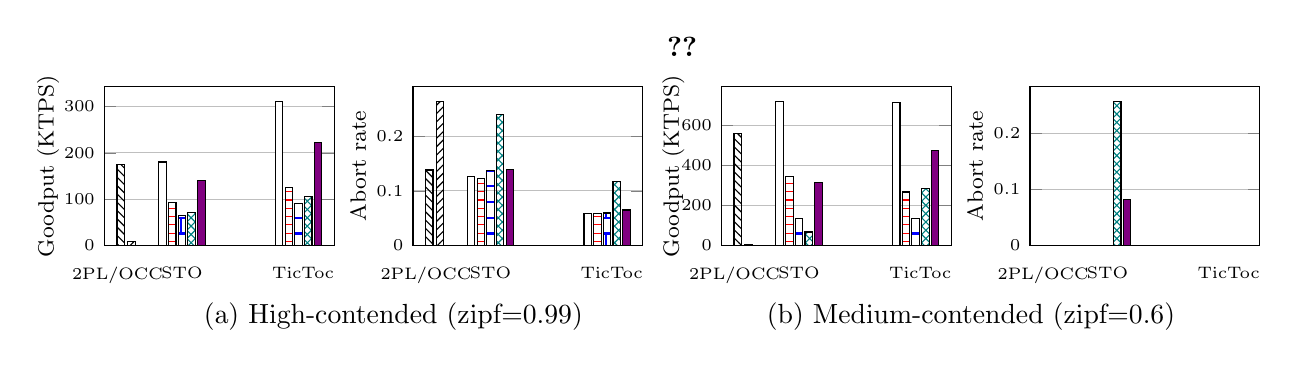
\begin{tikzpicture}
            \begin{groupplot}[group style={group size=4 by 1,
                            /pgf/bar width=2.7pt},
                    height = 3.6cm,
                    width = 4.5cm,
                    ybar= 2*\pgflinewidth,
                    xtick={-1, 0.425, 3.1},
                    xticklabels={2PL/OCC, STO, TicToc},
                    ymajorgrids=true,
                    enlarge x limits = 0.225,
                    legend columns=-1,
                    legend entries={{\ssmall Memory (Idealized)}, {\ssmall Disk}, {\ssmall Disk-Cache}, {\ssmall \fsketchname},  {\ssmall \psketchname}},
                    area legend,
                    legend to name=grouplegend,
                ]

                % graph [1,1] high
                \nextgroupplot[YCSBThroughputBarChartPlot, ylabel={Goodput (KTPS)}, ylabel style={yshift=-5pt}]
                \addplot[2PL-BarStyle, forget plot] coordinates {(-0.5, 174.950333)};
                \addplot[KR-OCC-BarStyle, forget plot] coordinates {(-0.26, 9.13111)};
                \addplot[Memory-BarStyle] coordinates {(0.425, 180.33) (3, 311.536)};
                \addplot[Disk-BarStyle] coordinates {(0.425, 92.825067) (3, 125.022333)};
                \addplot[Disk-Cache-BarStyle] coordinates {(0.425, 64.094933) (3, 91.446867)};
                \addplot[Counter-Lazy-BarStyle] coordinates {(0.425, 71.368433) (3, 105.553667)};
                \addplot[FPSketch-BarStyle] coordinates {(0.425, 140.384333) (3, 221.610333)};
                \coordinate (top) at (rel axis cs:0,1);% coordinate at top of the first plot

                % graph [2,1] abort rate
                \nextgroupplot[AbortRateBarChartPlot, ylabel={Abort rate}, ylabel style={yshift=-3pt}]
                \addplot[2PL-BarStyle, forget plot] coordinates {(-0.5, 0.138208)};
                \addplot[KR-OCC-BarStyle, forget plot] coordinates {(-0.26, 0.263853)};
                \addplot[Memory-BarStyle] coordinates {(0.425, 0.126144) (3, 0.058634)};
                \addplot[Disk-BarStyle] coordinates {(0.425, 0.122566) (3, 0.057911)};
                \addplot[Disk-Cache-BarStyle] coordinates {(0.425, 0.136498) (3, 0.059566)};
                \addplot[Counter-Lazy-BarStyle] coordinates {(0.425, 0.239943) (3, 0.117789)};
                \addplot[FPSketch-BarStyle] coordinates {(0.425, 0.139826) (3, 0.065083)};

                % graph [3,1] medium
                \nextgroupplot[YCSBThroughputBarChartPlot, ylabel={Goodput (KTPS)}, ylabel style={yshift=-8pt}]
                \addplot[2PL-BarStyle, forget plot] coordinates {(-0.5, 556.961)};
                \addplot[KR-OCC-BarStyle, forget plot] coordinates {(-0.26, 7.140063)};
                \addplot[Memory-BarStyle] coordinates {(0.425, 720.277667) (3, 714.753333)};
                \addplot[Disk-BarStyle] coordinates {(0.425, 345.637667) (3, 267.104333)};
                \addplot[Disk-Cache-BarStyle] coordinates {(0.425, 135.666333) (3, 134.658333)};
                \addplot[Counter-Lazy-BarStyle] coordinates {(0.425, 68.007267) (3, 284.942667)};
                \addplot[FPSketch-BarStyle] coordinates {(0.425, 315.562667) (3, 475.911667)};

                % graph [4,1] medium abort rate
                \nextgroupplot[AbortRateBarChartPlot, ylabel={Abort rate}, ylabel style={yshift=-3pt}]
                \addplot[2PL-BarStyle, forget plot] coordinates {(-0.5, 0.000335)};
                \addplot[KR-OCC-BarStyle, forget plot] coordinates {(-0.26, 0.000148)};
                \addplot[Memory-BarStyle] coordinates {(0.425, 0.000432) (3, 0.000202)};
                \addplot[Disk-BarStyle] coordinates {(0.425, 0.000239) (3, 0.000221)};
                \addplot[Disk-Cache-BarStyle] coordinates {(0.425, 0.000194) (3, 0.000078)};
                \addplot[Counter-Lazy-BarStyle] coordinates {(0.425, 0.257643) (3, 0.00023)};
                \addplot[FPSketch-BarStyle] coordinates {(0.425, 0.08147) (3, 0.000191)};
                \coordinate (bot) at (rel axis cs:1,0);% coordinate at bottom of the last plot

            \end{groupplot}
            \coordinate (c) at ($(top)!.5!(bot)$);
            \coordinate (cc1) at ($(top)!.25!(bot)$);
            \coordinate (cc2) at ($(top)!.75!(bot)$);

            \node[above] at (c |- current bounding box.north) {\ref{grouplegend}};
            \node[below] at (cc1 |- current bounding box.south) {(a) High-contended (zipf=0.99)};
            \node[above] at (cc2 |- current bounding box.south) {(b) Medium-contended (zipf=0.6)};
        \end{tikzpicture}
    } \caption[YCSB mixed-transaction workloads results on fast storage]{YCSB
    mixed-transaction workloads results with 120 processing threads on fast
    storage. 80\% of transactions perform 2 reads and 2 writes, and 20\% of
    transactions perform 28 reads. Note that, in the medium-contended workload,
    several variants have abort rates very close to 0.}
    \label{fig:ycsb:mixed_fast}
\end{figure}

\Cref{fig:ycsb:mixed_fast} presents the goodput outcomes for all timestamp-based
CC mechanisms across two mixed-transaction YCSB workloads under fast storage
conditions.

In the high-contention scenario, the trends of the different CC mechanisms are
similar to what we observed in the small-transaction workloads, but the
performance gaps are even larger. This is because mixed-transaction workloads
have a higher fraction of short transactions compared to the small-transaction
workloads. Looking at the numbers, TicToc-\psketchname achieves 1.78$\times$ and
24.3$\times$ higher throughput than 2PL and KR-OCC, respectively.
STO-\psketchname achieves 1.13$\times$ and 15.37$\times$ higher throughput than
2PL and KR-OCC, respectively. TicToc-\psketchname also reaches 77\% higher
goodput than TicToc-Disk, and STO-\psketchname is 51\% faster than STO-Disk.
However, when compared against the Memory configuration, both
TicToc-\psketchname and STO-\psketchname have 28\% and 22\% lower goodput,
respectively.

For the medium-contended scenario, there are two main points. First, similar to
the small-transaction experiments, 2PL still outperforms the \sketchname
variants, although the timestamp-based CC mechanisms running with Memory
configuration are still able to outperform 2PL. This shows that timestamping
itself is a strong approach. Second, in this situation, a Disk-based
configuration can outperform its \sketchname variant: STO-Disk achieves
1.09$\times$ faster than STO-\psketchname, while TicToc-\psketchname still
outperforms TicToc-Disk. This is the result of differences in abort handling:
STO aborts transactions immediately upon timestamp order break, while TicToc
waits until commit time to make this decision. This leads to more
over-approximation of timestamps in \sketchname for STO, especially since
mixed-transaction workloads have more short transactions. With bigger sketch
size than the evaluation setup, the abort rate of STO-\psketchname decreases.
For example, STO-\psketchname with 256KiB sketch size achieves approximately 520
KTPS, improving goodput by 50.4\% compared to STO-Disk. Thus, the more memory
for sketch is necessary for STO if transactions are short and their operations
are executed quickly.


\subsubsection{YCSB Long-Transaction Workload}


\begin{figure}[!t]
    \centering
    \resizebox{.75\textwidth}{!}{%
        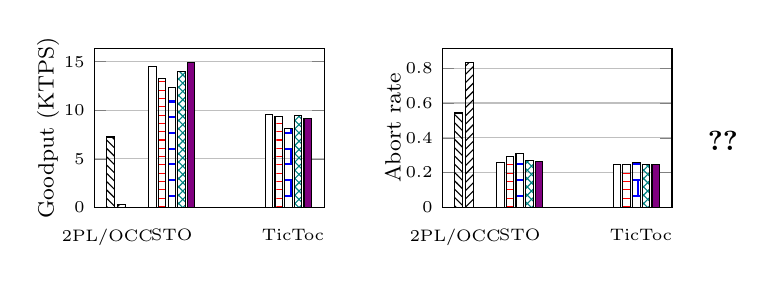
\begin{tikzpicture}
            \begin{groupplot}[group style={
                            group size=2 by 1,
                            horizontal sep=1.5cm,
                            /pgf/bar width=2.7pt
                        },
                    height = 3.6cm,
                    width = 4.5cm,
                    ybar= 2*\pgflinewidth,
                    xtick={-1, 0.425, 3.1},
                    xticklabels={2PL/OCC, STO, TicToc},
                    ymajorgrids=true,
                    enlarge x limits = 0.225,
                    legend columns=1,
                    legend entries={{\ssmall Memory (Idealized)}, {\ssmall Disk}, {\ssmall Disk-Cache}, {\ssmall \fsketchname},  {\ssmall \psketchname}},
                    area legend,
                    legend to name=grouplegend,
                ]

                % graph [1,1] high
                \nextgroupplot[YCSBThroughputBarChartPlot, ylabel={Goodput (KTPS)}, ylabel style={yshift=-5pt}]
                \addplot[2PL-BarStyle, forget plot] coordinates {(-0.5, 7.24927)};
                \addplot[KR-OCC-BarStyle, forget plot] coordinates {(-0.26, 0.275767)};
                \addplot[Memory-BarStyle] coordinates {(0.425, 14.4813) (3, 9.571037)};
                \addplot[Disk-BarStyle] coordinates {(0.425, 13.3011) (3, 9.311203)};
                \addplot[Disk-Cache-BarStyle] coordinates {(0.425, 12.304867) (3, 8.088823)};
                \addplot[Counter-Lazy-BarStyle] coordinates {(0.425, 13.978767) (3, 9.499523)};
                \addplot[FPSketch-BarStyle] coordinates {(0.425, 14.869067) (3, 9.124267)};
                \coordinate (top) at (rel axis cs:0,1);% coordinate at top of the first plot

                % graph [1,2] abort rate
                \nextgroupplot[AbortRateBarChartPlot, ylabel={Abort rate}, ylabel style={yshift=-5pt}]
                \addplot[2PL-BarStyle, forget plot] coordinates {(-0.5, 0.542658)}; % double check
                \addplot[KR-OCC-BarStyle, forget plot] coordinates {(-0.26, 0.829988)}; % double check
                \addplot[Memory-BarStyle] coordinates {(0.425, 0.260036) (3, 0.24408)}; % double check
                \addplot[Disk-BarStyle] coordinates {(0.425, 0.29484) (3, 0.248819)}; % double check sto
                \addplot[Disk-Cache-BarStyle] coordinates {(0.425, 0.307315) (3, 0.256368)}; % double check sto
                \addplot[Counter-Lazy-BarStyle] coordinates {(0.425, 0.267667) (3, 0.246097)}; % double check
                \addplot[FPSketch-BarStyle] coordinates {(0.425, 0.263106) (3, 0.247183)}; % double check
                \coordinate (bot) at (rel axis cs:1,0);% coordinate at bottom of the last plot

            \end{groupplot}
            \coordinate (c) at ($(top)!.5!(bot)$);

            \node[right=4cm] at (c |- current bounding box.east) {\ref{grouplegend}};
        \end{tikzpicture}
    } \caption[YCSB long-transaction workloads results on fast storage]{YCSB
    long-transaction workloads results with 120 processing threads on fast
    storage. 5\% of transactions perform 1000 reads and the rest of transactions
    perform 8 writes and 8 reads. The distribution is Zipfian with 0.9.}
    \label{fig:ycsb:long_fast}
\end{figure}

The results for long-transaction workloads in \Cref{fig:ycsb:long_fast} are
similar to those on other types of storage. On fast storage, STO and TicToc with
approximate timestamp storage reach goodput almost equal to their Memory
versions. This shows that approximate timestamps work well for both large and
small transactions on fast storage as well.

\subsubsection{TPC-C Workloads}

\begin{figure*}[!t]
    \centering
    \resizebox{\textwidth}{!}{%
        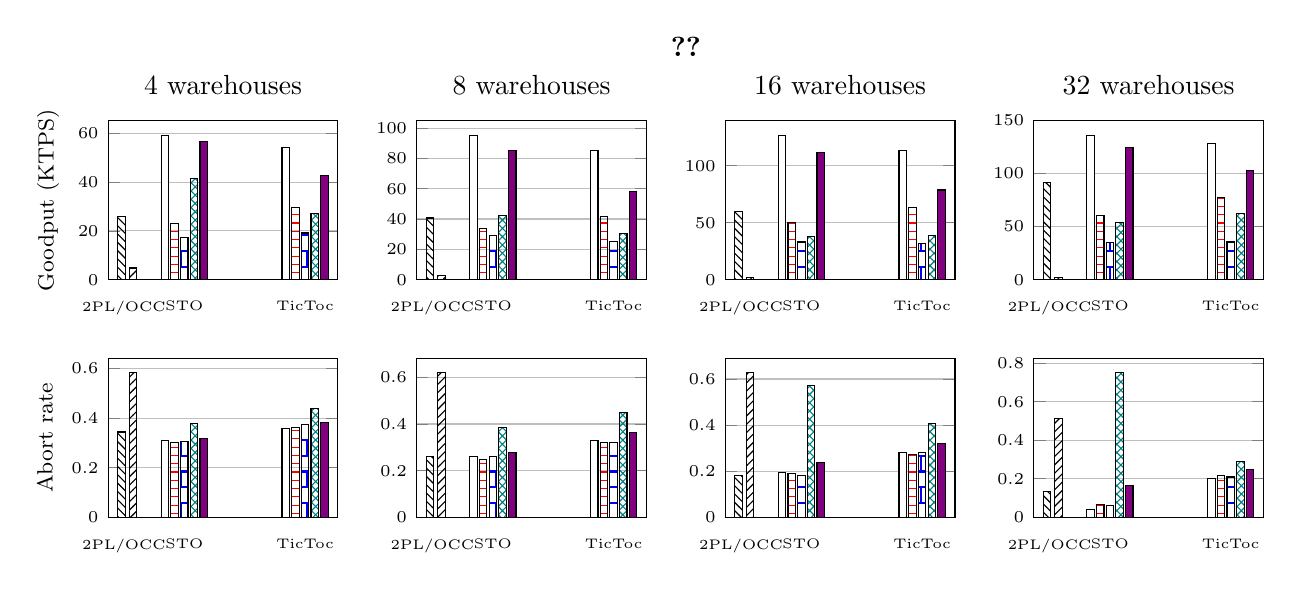
\begin{tikzpicture}
            \begin{groupplot}[group style={group size=4 by 2,
                            /pgf/bar width=2.7pt},
                    height = 3.6cm,
                    width = 4.5cm,
                    ybar= 2*\pgflinewidth,
                    xtick={-0.8625, 0.425, 3},
                    xticklabels={2PL/OCC, STO, TicToc},
                    xticklabel style={font=\tiny},
                    ymajorgrids=true,
                    enlarge x limits = 0.2,
                    legend columns=-1,
                    legend entries={{\ssmall Memory (Idealized)}, {\ssmall Disk}, {\ssmall Disk-Cache}, {\ssmall \fsketchname},  {\ssmall \psketchname}},
                    area legend,
                    legend to name=grouplegend,
                ]

                % graph [1,1]
                \nextgroupplot[title={4 warehouses},YCSBThroughputBarChartPlot, ylabel={Goodput (KTPS)}]
                \addplot[2PL-BarStyle, forget plot] coordinates {(-0.5, 25.981933)};
                \addplot[KR-OCC-BarStyle, forget plot] coordinates {(-0.26, 4.766923)};
                \addplot[Memory-BarStyle] coordinates {(0.425, 59.3193) (3, 54.249267)};
                \addplot[Disk-BarStyle] coordinates {(0.425, 23.122733) (3, 29.668767)};
                \addplot[Disk-Cache-BarStyle] coordinates {(0.425, 17.227167) (3, 19.149033)};
                \addplot[Counter-Lazy-BarStyle] coordinates {(0.425, 41.3587) (3, 27.051667)};
                \addplot[FPSketch-BarStyle] coordinates {(0.425, 56.8103) (3, 42.8906)};
                \coordinate (top) at (rel axis cs:0,1);% coordinate at top of the first plot

                % graph [1,2]
                \nextgroupplot[title={8 warehouses}, YCSBThroughputBarChartPlot]
                \addplot[2PL-BarStyle, forget plot] coordinates {(-0.5, 40.674833)};
                \addplot[KR-OCC-BarStyle, forget plot] coordinates {(-0.26, 2.690287)};
                \addplot[Memory-BarStyle] coordinates {(0.425, 95.317467) (3, 85.340067)};
                \addplot[Disk-BarStyle] coordinates {(0.425, 33.973233) (3, 41.828467)};
                \addplot[Disk-Cache-BarStyle] coordinates {(0.425, 29.014767) (3, 25.245733)};
                \addplot[Counter-Lazy-BarStyle] coordinates {(0.425, 42.335667) (3, 30.594867)};
                \addplot[FPSketch-BarStyle] coordinates {(0.425, 85.059467) (3, 58.450233)};

                % graph [1,3]
                \nextgroupplot[title={16 warehouses},YCSBThroughputBarChartPlot]
                \addplot[2PL-BarStyle, forget plot] coordinates {(-0.5, 60.0792)};
                \addplot[KR-OCC-BarStyle, forget plot] coordinates {(-0.26, 1.714923)};
                \addplot[Memory-BarStyle] coordinates {(0.425, 126.781667) (3, 113.534667)};
                \addplot[Disk-BarStyle] coordinates {(0.425, 49.8068) (3, 62.967367)};
                \addplot[Disk-Cache-BarStyle] coordinates {(0.425, 33.078067) (3, 31.654267)};
                \addplot[Counter-Lazy-BarStyle] coordinates {(0.425, 37.753067) (3, 38.951133)};
                \addplot[FPSketch-BarStyle] coordinates {(0.425, 111.767) (3, 78.6518)};


                % graph [1,4] 32wh
                \nextgroupplot[title={32 warehouses},YCSBThroughputBarChartPlot]
                \addplot[2PL-BarStyle, forget plot] coordinates {(-0.5, 91.371733)};
                \addplot[KR-OCC-BarStyle, forget plot] coordinates {(-0.26, 1.768823)};
                \addplot[Memory-BarStyle] coordinates {(0.425, 136.254) (3, 128.511333)};
                \addplot[Disk-BarStyle] coordinates {(0.425, 60.4086) (3, 77.2502)};
                \addplot[Disk-Cache-BarStyle] coordinates {(0.425, 35.204067) (3, 35.5132)};
                \addplot[Counter-Lazy-BarStyle] coordinates {(0.425, 54.0724) (3, 62.5415)};
                \addplot[FPSketch-BarStyle] coordinates {(0.425, 124.853) (3, 103.150333)};

                \coordinate (bot) at (rel axis cs:1,0);% coordinate at bottom of the last plot

                % graph [2,1] 4 wh
                \nextgroupplot[AbortRateBarChartPlot, ylabel={Abort rate}]
                \addplot[2PL-BarStyle, forget plot] coordinates {(-0.5, 0.343923)};
                \addplot[KR-OCC-BarStyle, forget plot] coordinates {(-0.26, 0.582189)};
                \addplot[Memory-BarStyle] coordinates {(0.425, 0.308396) (3, 0.358287)};
                \addplot[Disk-BarStyle] coordinates {(0.425, 0.300735) (3, 0.362429)};
                \addplot[Disk-Cache-BarStyle] coordinates {(0.425, 0.306576) (3, 0.373073)};
                \addplot[Counter-Lazy-BarStyle] coordinates {(0.425, 0.378139) (3, 0.439741)};
                \addplot[FPSketch-BarStyle] coordinates {(0.425, 0.316455) (3, 0.38327)};

                % graph [2,2] 8 wh
                \nextgroupplot[AbortRateBarChartPlot]
                \addplot[2PL-BarStyle, forget plot] coordinates {(-0.5, 0.26031)};
                \addplot[KR-OCC-BarStyle, forget plot] coordinates {(-0.26, 0.619373)};
                \addplot[Memory-BarStyle] coordinates {(0.425, 0.259365) (3, 0.328457)};
                \addplot[Disk-BarStyle] coordinates {(0.425, 0.249634) (3, 0.322022)};
                \addplot[Disk-Cache-BarStyle] coordinates {(0.425, 0.259498) (3, 0.320605)};
                \addplot[Counter-Lazy-BarStyle] coordinates {(0.425, 0.383305) (3, 0.448231)};
                \addplot[FPSketch-BarStyle] coordinates {(0.425, 0.279779) (3, 0.364156)};

                % graph [2,3] 16 wh
                \nextgroupplot[AbortRateBarChartPlot]
                \addplot[2PL-BarStyle, forget plot] coordinates {(-0.5, 0.181629)};
                \addplot[KR-OCC-BarStyle, forget plot] coordinates {(-0.26, 0.626907)};
                \addplot[Memory-BarStyle] coordinates {(0.425, 0.194619) (3, 0.282973)};
                \addplot[Disk-BarStyle] coordinates {(0.425, 0.189055) (3, 0.271532)};
                \addplot[Disk-Cache-BarStyle] coordinates {(0.425, 0.180874) (3, 0.280659)};
                \addplot[Counter-Lazy-BarStyle] coordinates {(0.425, 0.572401) (3, 0.40728)};
                \addplot[FPSketch-BarStyle] coordinates {(0.425, 0.23819) (3, 0.320579)};

                % graph [2,4] 32 wh
                \nextgroupplot[AbortRateBarChartPlot]
                \addplot[2PL-BarStyle, forget plot] coordinates {(-0.5, 0.133359)};
                \addplot[KR-OCC-BarStyle, forget plot] coordinates {(-0.26, 0.512981)};
                \addplot[Memory-BarStyle] coordinates {(0.425, 0.040332) (3, 0.202382)};
                \addplot[Disk-BarStyle] coordinates {(0.425, 0.067348) (3, 0.215892)};
                \addplot[Disk-Cache-BarStyle] coordinates {(0.425, 0.063018) (3, 0.20933)};
                \addplot[Counter-Lazy-BarStyle] coordinates {(0.425, 0.74949) (3, 0.291205)};
                \addplot[FPSketch-BarStyle] coordinates {(0.425, 0.167312) (3, 0.247521)};
            \end{groupplot}
            \coordinate (c) at ($(top)!.5!(bot)$);

            \node[above] at (c |- current bounding box.north) {\ref{grouplegend}};
        \end{tikzpicture}
    } \caption[TPC-C results on fast storage]{TPC-C results with 120 processing
    threads on fast storage (More warehouses means less contention).}
    \label{fig:tpcc_fast}
\end{figure*}

\Cref{fig:tpcc_fast} shows the TPC-C benchmark results on fast storage. The
figure includes both goodput and abort rates for different concurrency control
methods as we change the number of warehouses (which also changes the
contention level). Similar to the YCSB results, both \psketchname and
\fsketchname always have lower goodput than the Memory version because of extra
overheads, but they are still much better than the Disk-based methods.

TicToc-\psketchname achieves up to 9 to 58.3$\times$ higher goodput than
2PL/KR-OCC, and about 25--44.5\% higher goodput than TicToc-Disk at all
contention levels. STO-\psketchname achieves up to 11.9 to 70.6$\times$ more
goodput than 2PL/KR-OCC, and about 105--150\% improvement over STO-Disk in all
cases. The TPC-C benchmark consists of both short and long transactions, and STO
achieves higher goodput than TicToc for long transactions. This matches our
earlier findings from the YCSB long-transaction workload in
\Cref{fig:ycsb:long_fast}.

Comparing \psketchname and \fsketchname, we see that \psketchname always has
better goodput at every contention level. This is because \psketchname has less
overhead from sketch evictions. However, the gap between the two gets smaller
when the workload is less contentious (that is, when there are more warehouses).
This indicates that \psketchname is a good option for deployment on fast
storage.


\section{Summary}

This chapter presents a comprehensive evaluation of \sketchname across diverse
storage media, from traditional slow storage (SATA SSD and HDD) to modern fast
storage emulating CXL-based flash with DRAM-like latency. Our experimental study
reveals several important findings and lessons that guide the adoption and future
development of \sketchname.

\subsection{Key Findings}

Our evaluation demonstrates that \sketchname remains effective across a wide
range of storage technologies. On slow storage media, including SATA SSD and
HDD, \sketchname variants consistently achieve goodput close to the idealized
Memory configuration. The benefits are most pronounced in high-contention,
write-intensive workloads, where \sketchname improves goodput by up to 569\%
compared to Disk-based timestamp storage on SATA SSD and up to 519\% on HDD.
Even in medium-contention scenarios where storage I/O becomes the primary
bottleneck, \sketchname still provides substantial improvements by eliminating
the overhead of accessing timestamps from disk.

On fast storage media, our experiments reveal a different set of
characteristics. Timestamp-based concurrency control methods, when combined with
\sketchname, significantly outperform 2PL and KR-OCC because they enable higher
concurrency and result in fewer transaction aborts. For instance,
TicToc-\psketchname achieves up to 3.55$\times$ and 21.5$\times$ higher goodput
than 2PL and KR-OCC, respectively, in high-contention, read-intensive workloads.
However, \sketchname variants do not reach the performance of the idealized
Memory configuration due to overhead from their operations, memory allocation,
and key management in the \sketchname data structure itself.

\subsection{Lessons Learned}

Our experimental study yields several important lessons. First, the effectiveness
of \sketchname varies with storage characteristics. On slow storage, where disk
I/O dominates performance, \sketchname provides substantial benefits by removing
the need to access timestamps from persistent storage. On fast storage, while
\sketchname still outperforms Disk-based approaches, the relative overhead of
the \sketchname data structure becomes more visible. This suggests that future
optimizations should focus on reducing this overhead, particularly for
high-performance storage environments.

Second, we observe that \psketchname consistently outperforms \fsketchname
across all storage types and workloads. The additional overhead of evicting keys
to the sketch in \fsketchname creates a performance gap that becomes more
pronounced as storage becomes faster. Moreover, \psketchname also outperforms
Disk-based configurations in the vast majority of scenarios, making it the clear
preferred choice among all timestamp storage options. Only in rare cases with
medium-contention scenarios on fast storage can Disk-based configurations
occasionally match or slightly exceed \psketchname performance, when the
overhead of maintaining the sketch outweighs the benefits of avoiding disk
accesses. In practice, these cases are limited, and \psketchname offers superior
performance while still eliminating the need to access timestamps from
persistent storage.

Third, our results highlight the importance of transaction characteristics in
determining \sketchname's effectiveness. Short transactions with quick
operations benefit more from \sketchname, especially on slow storage. For long
transactions, the impact is smaller because the transaction execution time
dominates, but \sketchname still provides improvements by reducing timestamp
access overhead. The mixed-transaction workloads demonstrate that \sketchname
maintains its effectiveness even when workloads contain both short and long
transactions.

Finally, our evaluation reveals that storage media characteristics fundamentally
change the performance trade-offs in concurrency control. As storage becomes
faster, timestamp-based methods with \sketchname emerge as the clear winners
over traditional locking-based approaches. This finding suggests that as storage
technology continues to evolve toward lower latency and higher bandwidth,
\sketchname will become increasingly important for enabling high-performance
transaction processing in disk-based key-value stores.

\subsection{Deployment Guidelines}

Based on our comprehensive evaluation, we offer the following deployment
guidelines for \sketchname:

\textbf{Variant selection:} \psketchname should be preferred over \fsketchname in
virtually all scenarios, as it consistently outperforms \fsketchname across all
storage types and workloads while requiring similar memory footprint. The only
exception is when memory constraints are extremely tight and the workload has very
low contention, where \fsketchname's ability to evict keys might provide marginal
memory savings.

\textbf{Storage-specific recommendations:} On slow storage (SATA SSD and HDD),
\sketchname provides dramatic improvements and should be adopted whenever 
timestamp-based CC methods are used. The benefits are most pronounced for 
high-contention workloads. On fast storage (CXL-based flash or similar), 
\sketchname remains beneficial, particularly for high-contention scenarios where
timestamp-based methods significantly outperform 2PL and KR-OCC. However, the
overhead becomes more visible, suggesting future optimization opportunities.

\textbf{Workload considerations:} \sketchname is most beneficial for workloads with
short transactions and high contention, especially write-intensive operations. For
long transactions, \sketchname still provides improvements, but the impact is
smaller since transaction execution time dominates. Mixed workloads benefit
substantially from \sketchname across all storage types.

\textbf{Memory requirements:} \sketchname requires minimal memory (32KiB in our
experiments with an 80GB database), making it practical for deployment even in
memory-constrained environments. This footprint remains consistent across storage
types, as the sketch size is workload-dependent rather than storage-dependent.

\textbf{Concurrency control pairing:} TicToc with \psketchname consistently
provides the best performance across all evaluated scenarios, making it the
recommended combination for new deployments. STO with \psketchname is also
excellent, particularly for long transactions. MVTO can benefit from \sketchname
on slow storage, but may face memory limitations on fast storage with 
write-intensive workloads.

In conclusion, \sketchname proves to be a valuable technique for enabling modern
timestamp-based concurrency control methods on persistent storage across a wide
spectrum of storage technologies. While there are opportunities for further
optimization, particularly for fast storage environments, the experimental
evidence strongly supports the adoption of \sketchname in production systems
that use various storage media.


\chapter{Related Work}
\label{chapter:five}
\section{Forgetful STO}

Bernstein, et al.~\cite{bernstein1987concurrency} attempted to reduce the memory
footprint of STO by proposing a timestamp purge mechanism. The approach assumes
that timestamps are derived from a reasonably precise real-time clock and that
transactions are short-lived. Their approach involves selecting a threshold
timestamp ($\tau - \delta$) at $\tau$, purging keys with timestamps below this
threshold from memory, tagging these keys with the threshold timestamp, and
aborting any transactions whose timestamp is below the threshold. Effectively,
this overapproximates the purged keys' timestamps to the threshold timestamp.
While Bernstein, et al.~argued that this was safe to do, they did not specify
any policy for how to select the threshold timestamp that determines which keys
get evicted. Such a policy is crucial to balancing memory usage and abort rate.
They did not implement or evaluate their scheme.

Bernstein's approach does not meet the requirements of an approximate timestamp
storage system defined in \Cref{sec:requirements}; it sometimes approximates
timestamps of keys in use by on-going transactions, aborting those transactions.
This works with STO and MVTO but, surprisingly, aborting the transactions of the
affected keys is not sufficient to guarantee serializability in TicToc!

Below are two examples that illustrate this issue based on TicToc's validation
algorithm~\cite{yu2016tictoc}.

\paragraph{Example 1:} Consider these transactions:

\begin{tabular}{|l|l|l|l|}
    \hline
    \textbf{Step} & \textbf{TID} & \textbf{Operation}        & \textbf{Note}                           \\
    \hline
    1             & $T_1$        & read($k_1$)               & $k_1.rts=10$, $k_1.wts=10$              \\
    2             & $T_2$        & write($k_1$), lock($k_1$) & $commit\_ts=11$                         \\
    3             & $T_1$        & write($k_2$), lock($k_2$) & $commit\_ts=12$                         \\
    4             & $T_1$        & abort                     & $k_1.tuple.rts \leq commit\_ts$ $\land$
    isLocked($k_1$) $\land$ $k_1$ not in $W$                                                           \\
    5             & $T_2$        & commit                    &                                         \\
    \hline
\end{tabular}

Initially, $k_1$ has $k_1.tuple.rts=10$ and $k_1.tuple.wts=10$ in the database.
Here, $k_1.tuple.*$ refers to database values, while $k_1.*$ refers to
transaction-local values. Let's examine each step in detail:

\begin{enumerate}
    \item $T_1$ reads $k_1$, recording $k_1.rts=10$, $k_1.wts=10$.
    \item $T_2$ writes to $k_1$, locks it, and sets $commit\_ts=11$
          during validation.
    \item $T_1$ writes to $k_2$, locks it, and sets $commit\_ts=12$
          during validation.
    \item $T_1$ aborts because another transaction ($T_2$) is
          validating $k_1$. The abort condition is met when:
          \begin{itemize}
              \item $k_1.tuple.rts=10 \leq commit\_ts=12$ (true)
              \item $k_1$ is locked (true)
              \item $k_1$ is not in $T_1$'s write set (true)
          \end{itemize}
    \item $T_2$ commits with $commit\_ts=11$.
\end{enumerate}

TicToc maintains serializability by aborting $T_1$, which would otherwise read
outdated data.

However, if timestamp purging occurs during validation, serializability can be
violated. Suppose keys with timestamps less than 20 are purged before Step 4,
setting $k_1.tuple.rts$ to 20. (This can happen because TicToc processes
transactions based on keys accessed by them in a lazy and distributed manner
while the purge system would keep track of the largest timestamp of all keys and
pick 20 as a safe threshold timestamp.) Since $T_1$ already set $commit\_ts=12$,
the validation check will now fail ($k_1.tuple.rts=20 > commit\_ts=12$),
allowing $T_1$ to commit with $commit\_ts=12$. Then $T_2$ commits with
$commit\_ts=11$. This violates serializability because $T_1$ reads an old
version but is serialized after $T_2$.

\paragraph{Example 2:} Consider these transactions:

\begin{tabular}{|l|l|l|l|}
    \hline
    \textbf{Step} & \textbf{TID} & \textbf{Operation}        & \textbf{Note}                       \\
    \hline
    1             & $T_1$        & write($k_1$), lock($k_1$) & $k_1.tuple.rts=10$                  \\
    2             & $T_2$        & read($k_1$)               & $k_1.rts=10$, $k_1.wts=10$          \\
    3             & $T_2$        & write($k_1$)              &                                     \\
    4             & $T_1$        & commit                    & $commit\_ts=11$, $k_1.tuple.wts=11$ \\
    5             & $T_2$        & abort                     & $k_1.wts \neq k_1.tuple.wts$        \\
    \hline
\end{tabular}

Initially, $k_1$ has $k_1.tuple.rts=10$ and $k_1.tuple.wts=10$.
Here is an explanation of each step:

\begin{enumerate}
    \item $T_1$ writes to $k_1$.
    \item $T_2$ reads $k_1$, recording $k_1.rts=10$, $k_1.wts=10$.
    \item $T_2$ writes to $k_1$. ($commit\_ts$ will be 11.)
    \item $T_1$ commits with $commit\_ts=11$ and updates $k_1.tuple.wts=11$.
    \item $T_2$ aborts because it detects a version mismatch:
          \begin{itemize}
              \item $k_1.tuple.wts=11 \neq k_1.wts=10$ (true)
          \end{itemize}
\end{enumerate}

$T_2$ correctly aborts after detecting a new version through the updated write
timestamp. However, if timestamp purging happens after Step 1, purging keys with
timestamps below 11 and updating both $k_1.tuple.rts$ and $k_1.tuple.wts$ to 11,
serializability is broken. In Step 2, $T_2$ would read $k_1.rts=11$,
$k_1.wts=11$. When $T_1$ commits with $commit\_ts=11$, $T_2$ proceeds to commit
with $commit\_ts=12$ (calculated as $k_1.tuple.rts + 1$). Since
$k_1.tuple.wts=11$ matches $k_1.wts=11$, $T_2$ cannot detect the version change
and incorrectly commits with $commit\_ts=12$. This breaks serializability
because $T_2$ reads a stale version yet is serialized after $T_1$.

Therefore, Bernstein's scheme itself without tracking in-use keys is
incompatible with TicToc because accurate timestamp data is critical during
validation, and TicToc relies on decentralized, fine-grained validation.


\section{On-Disk Concurrency Control}

Conventional concurrency control mechanisms, such as two-phase locking
(2PL) and optimistic concurrency control (OCC), are widely employed by
both academic and commercial disk-based
databases~\cite{rocksdb,googlef1,leveldb,asterixdb,cstore,berkeleydb,couchbase,asuresql}.
For example, RocksDB supports both pessimistic and optimistic
concurrency controls through 2PL and OCC, while Google F1 (Spanner)
uses timestamp ordering with locks and OCC. In contrast, there has
been significant research on concurrency control mechanisms tailored
for in-memory databases~\cite{yu2016tictoc}. \sketchname brings modern
concurrency control algorithms to disk-based transactional databases,
including those originally designed for in-memory contexts, instead of
relying solely on classical methods.

\section{Timestamp Access Acceleration}

Many disk-based RDBMSs (e.g., Postgres and MySQL) and write-optimized
systems (e.g., RocksDB) embed timestamps in their tuple structures,
thereby avoiding extra I/O once the relevant pages are in memory.
Recent studies on Bf-Tree~\cite{DBLP:journals/pvldb/HaoC24} and
Umbra~\cite{umbra-cc} highlight the critical role of efficient page
cache management in boosting performance, as on-disk timestamps can be
fetched quickly once loaded. By contrast, our approach decouples
timestamps from on-disk tuple structures and stores them in FPSketch.
This design not only accelerates timestamp operations of CCs but also
offers greater opportunities for high cache utilization of records on
disk. We believe that transactional systems leveraging FPSketch can
attain even stronger performance gains when paired with robust page
cache management.

\section{Approximation and Summarization in Databases}

Numerous databases approximate or summarize transaction metadata in
order to optimize I/O or reduce memory usage.  For example, PostgreSQL
maintains hintbits~\cite{postgres-visibility} in each tuple,
indicating whether the transction that added that tuple has committed,
enabling it to avoid a query to its commit log.  AWS Aurora maintains
Min Read Point LSNs~\cite{VerbitskiGuSa17}, which conservatively
indicate the oldest LSN that might still be read, enabling garbage
collection of pages with older LSNs.  And many MVCC schemes use high
watermarks~\cite{BottcherLeNe19} to determine which old versions can
be garbage collected.

We believe \sketchname is fundamentally different from prior work
because, in all these prior schemes, approximations and summations are
used as fast paths (e.g. hintbits) or to drive garbage collection.
However, they are not used as part of the CC mechanism itself.

\section{Approximation with Sketches}

In networking, FlexSwitch~\cite{flexswitch} uses an approximation
technique called min-timestamp to manage packet routing through
network switches. However, min-timestamp operates by overwriting
conflicting timestamps without guaranteeing a lower bound for these
values, allowing overwrites to occur at any time by any entity. In
contrast, \sketchname ensures monotonically increasing timestamps.
Additionally, it provides high-resolution timestamps that can be
shared among active transactions. This not only maintains correctness
in timestamp-based concurrency control mechanisms but also optimizes
space utilization.


\chapter{Conclusion and Future Work}
\label{chapter:six}
\section{Summary of Contributions}

This dissertation addresses a fundamental challenge in modern database systems:
enabling efficient timestamp-based concurrency control in disk-based
transactional databases. Through both theoretical analysis and experimental
evaluation, we demonstrate that approximate timestamp storage represents a
universal and future-ready approach for high-performance transaction processing
across diverse storage media technologies.

Our work makes two primary contributions. First, we introduce \sketchname, a
novel approximate timestamp storage system that enables efficient
timestamp-based concurrency control in disk-based key-value stores. \sketchname
combines a hash table for exact timestamps of active keys with a sketch for
approximate upper bounds of inactive keys, achieving the performance benefits of
fully in-memory timestamp storage while requiring only minimal memory—as little
as 32KiB for an 80GB database. Second, we conduct a comprehensive analytical and
experimental study demonstrating that \sketchname remains effective across a
wide spectrum of storage technologies, from traditional hard disk drives with
millisecond latencies to emerging CXL-based storage approaching DRAM-like
speeds.

\subsubsection{The \sketchname System}

The first contribution establishes \sketchname as a practical solution to the
metadata storage problem in timestamp-based concurrency control. Our design is
grounded in a key insight: for timestamp-based protocols like STO, MVTO, and
TicToc, overapproximating timestamps does not violate correctness—it may cause
harmless extra aborts but preserves serializability. This insight allows us to
use approximate data structures while maintaining all correctness guarantees.

\sketchname's hybrid architecture, combining a foveated region (hash table) and
peripheral region (sketch), ensures that active keys maintain exact timestamps
throughout their transaction lifetime while inactive keys can be safely
approximated. We formally prove that this approach satisfies the necessary
properties for correctness with all three protocols we studied. Our evaluation
demonstrates that \sketchname-based implementations achieve dramatic performance
improvements: TicToc with \psketchname improves goodput by up to 5.9$\times$
over disk-based timestamp storage, up to 14$\times$ over traditional 2PL, and
reaches performance close to an idealized in-memory system.

\subsubsection{Broad Applicability Across the Storage Spectrum}

The second contribution establishes the universal applicability of the
approximate timestamp storage approach. Our comprehensive evaluation across
HDDs, SATA SSDs, NVMe SSDs, and simulated CXL-based storage reveals that
\sketchname's benefits scale with the fundamental gap between local memory and
remote storage access. This finding ensures that \sketchname will remain
valuable as storage technology continues to evolve.

On slow storage (HDDs and SATA SSDs), where disk I/O dominates performance,
\sketchname eliminates the prohibitive overhead of timestamp disk accesses. Our
results show improvements of up to 569\% on SATA SSD and 519\% on HDD compared
to disk-based timestamp storage in high-contention, write-intensive workloads.
Even in medium-contention scenarios where storage I/O is the primary bottleneck,
\sketchname provides substantial improvements.

On fast storage (simulated DRAM-like speed of CXL-based SSDs), the performance
characteristics undergo a fundamental shift: the system transitions from being
I/O-bound to CPU-bound as storage latencies approach the single-digit
microsecond range. This transition makes the overhead of \sketchname's data
structure operations (hash table management, memory allocation, and sketch
operations) more visible relative to storage access costs. However, \sketchname
continues to provide substantial benefits by eliminating timestamp access
overhead through persistent storage, and more importantly, timestamp-based
concurrency control methods combined with \sketchname significantly outperform
traditional approaches. Specifically, TicToc-\psketchname achieves up to
3.55$\times$ and 21.5$\times$ higher goodput than 2PL and KR-OCC, respectively,
in high-contention workloads on fast storage, demonstrating that timestamp-based
methods enable higher concurrency and fewer aborts when storage is no longer the
limiting factor. While \sketchname variants do not reach the performance of
idealized in-memory timestamp storage due to their internal overhead, they still
deliver dramatic improvements over disk-based approaches and traditional
concurrency control methods across the entire storage spectrum.

 
 

\section{Key Findings and Insights}

Our research yields several important findings that guide both current
deployment and future development:

\subsubsection{Performance Characteristics}

Across all evaluated storage technologies and workloads, \sketchname
consistently outperforms traditional concurrency control methods and disk-based
timestamp storage. The \psketchname variant achieves goodput close to the
idealized Memory configuration while using only a tiny fraction of memory.
TicToc with \psketchname emerges as the clear performance leader, significantly
outperforming other concurrency control methods across all scenarios.

The memory efficiency of \sketchname is remarkable: a 32KiB sketch suffices for
an 80GB database, representing less than 0.00004\% of the database size. This
efficiency makes \sketchname practical even in memory-constrained environments
where storing all timestamps in RAM would be infeasible.

\subsubsection{Storage-Dependent Behavior}

Our analysis reveals that the nature of \sketchname's advantages changes
fundamentally as storage performance improves. On slow storage, \sketchname
primarily eliminates I/O bottlenecks, achieving performance close to idealized
in-memory systems. On fast storage, while \sketchname still effectively
eliminates the overhead of accessing timestamps from disk, the CPU overhead from
sketch operations becomes more visible, creating optimization opportunities for
future work.

\subsubsection{Workload Sensitivity}

\sketchname demonstrates consistent effectiveness across diverse workloads, from
small transactions typical of OLTP systems to long transactions.
High-contention, write-intensive workloads show the largest improvements, but
even medium-contention scenarios benefit substantially. Mixed workloads
containing both short and long transactions maintain \sketchname's
effectiveness, demonstrating its robustness.

\subsubsection{Protocol Compatibility}

Our formal analysis and experimental evaluation confirm that \sketchname
correctly integrates with STO, MVTO, and TicToc without any algorithmic changes
to these protocols. This plug-and-play compatibility makes adoption
straightforward and suggests that \sketchname could similarly integrate with
other timestamp-based protocols or future innovations in concurrency control.

\section{Broader Implications}

The success of \sketchname points to a broader principle: approximate metadata
management can enable high-performance system designs that would otherwise be
impractical. The key insight—that overapproximation preserves correctness for
many concurrency control protocols—may find application beyond timestamp
storage.

As storage technologies continue evolving toward faster, more memory-like
interfaces, the distinction between memory and storage blurs. \sketchname
demonstrates how application-specific caching strategies can bridge this gap,
providing a template for managing other types of frequently accessed metadata in
future systems.

Our work also highlights an important shift in database system design.
Traditional systems optimized for disk I/O as the dominant bottleneck. Modern
systems must optimize for CPU efficiency and memory hierarchy utilization.
\sketchname exemplifies this new design paradigm by prioritizing CPU and memory
efficiency while maintaining correctness guarantees.

\section{Future Work}

While \sketchname demonstrates strong performance across diverse storage
technologies, several directions offer opportunities for further improvement and
broader application.

\subsubsection{Optimizations for Fast Storage}

Our evaluation reveals that on fast storage (CXL-based or similar), \sketchname
incurs CPU overhead from sketch operations, memory allocation, and key
management that prevents it from fully matching the idealized Memory
configuration. Future work could explore several optimization strategies:

First, \emph{lock-free and wait-free algorithms} could reduce synchronization
overhead in the sketch and hash table operations. Current implementations use
per-bucket locks which, while correct, may become bottlenecks on fast storage
where operations complete in nanoseconds.

Second, \emph{custom memory allocators} optimized for the access patterns of
\sketchname could reduce allocation overhead. Fast storage environments are
CPU-bound, making efficient memory management critical.

Third, \emph{hardware acceleration} could leverage modern CPU features like SIMD
instructions for bulk sketch operations or hardware transactional memory for
lock-free updates. Exploring how emerging CPU architectures can accelerate
\sketchname operations presents an interesting research direction.

Finally, \emph{adaptive sketch sizing} could dynamically adjust sketch size
based on workload characteristics, reducing overhead for low-contention
scenarios while maintaining accuracy for high-contention workloads.

\subsubsection{Integration with Distributed Systems}

This dissertation focuses on single-node systems, but many production databases
operate in distributed environments. Extending \sketchname to distributed
systems raises several research questions:

How should timestamps be synchronized across nodes while maintaining
\sketchname's efficiency? Distributed timestamp allocation introduces
coordination overhead that could negate \sketchname's benefits. Research into
lightweight distributed timestamp protocols compatible with \sketchname would be
valuable.

Can each node maintain its own \sketchname instance for local keys? This
approach seems promising for shared-nothing architectures where transactions
primarily access local partitions. However, cross-partition transactions may
require different strategies.

How do network latencies affect the trade-offs that make \sketchname beneficial?
In distributed systems, network communication often dominates latency,
potentially changing the relative importance of local timestamp access
optimization.

\subsubsection{Advanced Concurrency Control Protocols}

While we demonstrate \sketchname's compatibility with STO, MVTO, and TicToc,
many other timestamp-based protocols exist. Investigating compatibility with
protocols like Serializable Snapshot Isolation (SSI), variations of OCC with
timestamps, or hybrid approaches could broaden \sketchname's applicability.

More fundamentally, could \sketchname inspire new concurrency control protocols
designed explicitly for approximate timestamp storage? The guarantees provided
by \sketchname may enable protocols that are not feasible with exact timestamps.

\subsubsection{Integration with Existing Database Systems}

While we evaluate \sketchname with SplinterDB, integration with other storage
systems would validate broader applicability. Integrating \sketchname with
LSM-tree based systems like RocksDB, B-tree systems like PostgreSQL, or other
storage architectures could reveal system-specific optimization opportunities.

Particularly interesting would be integration with systems that already maintain
some form of timestamp or version metadata, such as multi-version concurrency
control systems. Could \sketchname replace or enhance existing timestamp
management mechanisms?

\subsubsection{Other Storage Technologies}

Our evaluation covers HDD, SATA SSD, NVMe SSD, and simulated CXL-based storage,
but storage technology continues evolving. Evaluating \sketchname with emerging
future storage technologies would validate its continued relevance.

As storage becomes faster and more memory-like, understanding the point at which
approximate timestamp storage becomes unnecessary would provide important design
guidance. This transition point may depend on workload characteristics, system
architecture, and economic factors.

\subsubsection{Evaluation on Real CXL-based SSDs}

While our study includes a simulation of CXL-class latencies, an important next
step is to evaluate \sketchname on production CXL-connected devices. Real
hardware introduces effects that are difficult to capture in simulation,
including PCIe/CXL fabric contention, device firmware policies (e.g., interrupt
moderation, internal queueing, and thermal throttling), host driver and I/O
stack interactions, and tail-latency behaviors under bursty workloads. A
systematic experimental campaign on commercially available CXL-based SSDs and
memory expanders would (1) validate our analytical model and calibrate
constants, (2) quantify head- and tail-latency distributions and CPU overheads
at varying queue depths, NUMA placements, and PCIe topologies, and (3) surface
optimization opportunities specific to CXL (e.g., larger submission queues,
batching, and polling). These results would strengthen external validity and
refine guidance for deploying \sketchname on next-generation storage.

\subsubsection{Beyond Timestamps: General Approximate Metadata}

The principle underlying \sketchname—that approximate metadata can preserve
correctness for certain protocols—may apply beyond timestamps. Could similar
techniques optimize storage of locks, version numbers, conflict detection
metadata, or other concurrency control state?

Exploring the space of metadata that can be safely approximated could yield
additional optimization opportunities. This direction requires identifying
metadata properties that allow approximation without violating correctness.

\subsubsection{Workload-Aware Optimization}

Our evaluation demonstrates that \sketchname's effectiveness varies with
workload characteristics. Future work could develop \emph{adaptive \sketchname}
variants that automatically adjust their behavior based on observed workload
patterns. For example, sketch size could adapt to contention levels, eviction
policies could optimize for observed access patterns, or the hash table could
resize based on active key counts.

Machine learning techniques could potentially optimize \sketchname parameters
based on historical workload data, automatically tuning for best performance
without manual intervention.

\section{Concluding Remarks}

This dissertation demonstrates that approximate timestamp storage enables
efficient timestamp-based concurrency control in disk-based databases while
requiring minimal memory. Through the design and evaluation of \sketchname, we
establish that this approach remains effective across a wide spectrum of storage
technologies, from traditional hard drives to emerging memory-like storage.

The key contribution of this work is not merely a new data structure, but a
demonstration that approximate metadata management can unlock high-performance
system designs that would otherwise be impractical. As storage technology
continues evolving and the gap between memory and storage narrows, techniques
like \sketchname that optimize metadata access will become increasingly
important for achieving optimal database performance.

\sketchname represents a practical, deployable solution to a fundamental
challenge in modern database systems. By requiring only 32KiB of memory for an
80GB database while achieving performance close to idealized in-memory systems,
\sketchname makes advanced concurrency control protocols accessible to
real-world database deployments. The universal applicability of \sketchname
across storage technologies ensures its relevance both today and as storage
continues evolving.

More broadly, this work contributes to a paradigm shift in transactional system
design, from optimizing for disk I/O to optimizing for CPU efficiency and memory
hierarchy utilization. As this shift continues, approximate metadata management
techniques will play an increasingly central role in high-performance
transaction processing.



\bibliography{main.bib}
\bibliographystyle{acl_natbib}

% Optionally: add appendices
% \newpage
% \newcommand{\beginsupplement}{%
%     \setcounter{chapter}{0}
%     \renewcommand{\thechapter}{\Alph{chapter}}%
%  }

% \beginsupplement
% \chapter{Appendix One}
% \section{Appendix section 1}
% \begin{table}[]
%     \centering
%     \begin{tabular}{c|c}
%          &  \\
%          & 
%     \end{tabular}
%     \caption{Table in the Appendix}
%     \label{tab:my_label}
% \end{table}

\end{document}

% you're all done, congrats!